\chapter{Deep Radiomics for histological grade prediction}

\section{Semantic segmentation applied to weakly annotated datasets}

We proved that semantic segmentation of liver tissues can be
performed using \ac{dl} through robust CV training on both \textbf{\lmttfont{3DIrcad-dB}} and
\textbf{\lmttfont{TheraHCC-dB}}.
We also demonstrated that both a cascaded architecture and the use of
multiphase information allows a better segmentation accuracy than using
single phase images only.
We will now extend our work to prove the ability of semantic segmentation architecture to provide missing annotations into weakly annotated datasets such as \textbf{\lmttfont{TCIA-dB}}.\\
\textbf{\lmttfont{TCIA-dB}} originally only
contained raw images without annotations, so an expert performed the
delineations for both the tumor and the necrosis areas on \ac{pv} images only. \\
To achieve a multiphasic semantic segmentation of the liver tissues we
have to ensure that both the liver and its internal structures such as
the potential tumors are located at the same spatial position between
the different \ac{cect} volumes.


\subsection{Registration}\label{registration}

\begin{figure}[th!]
\centering
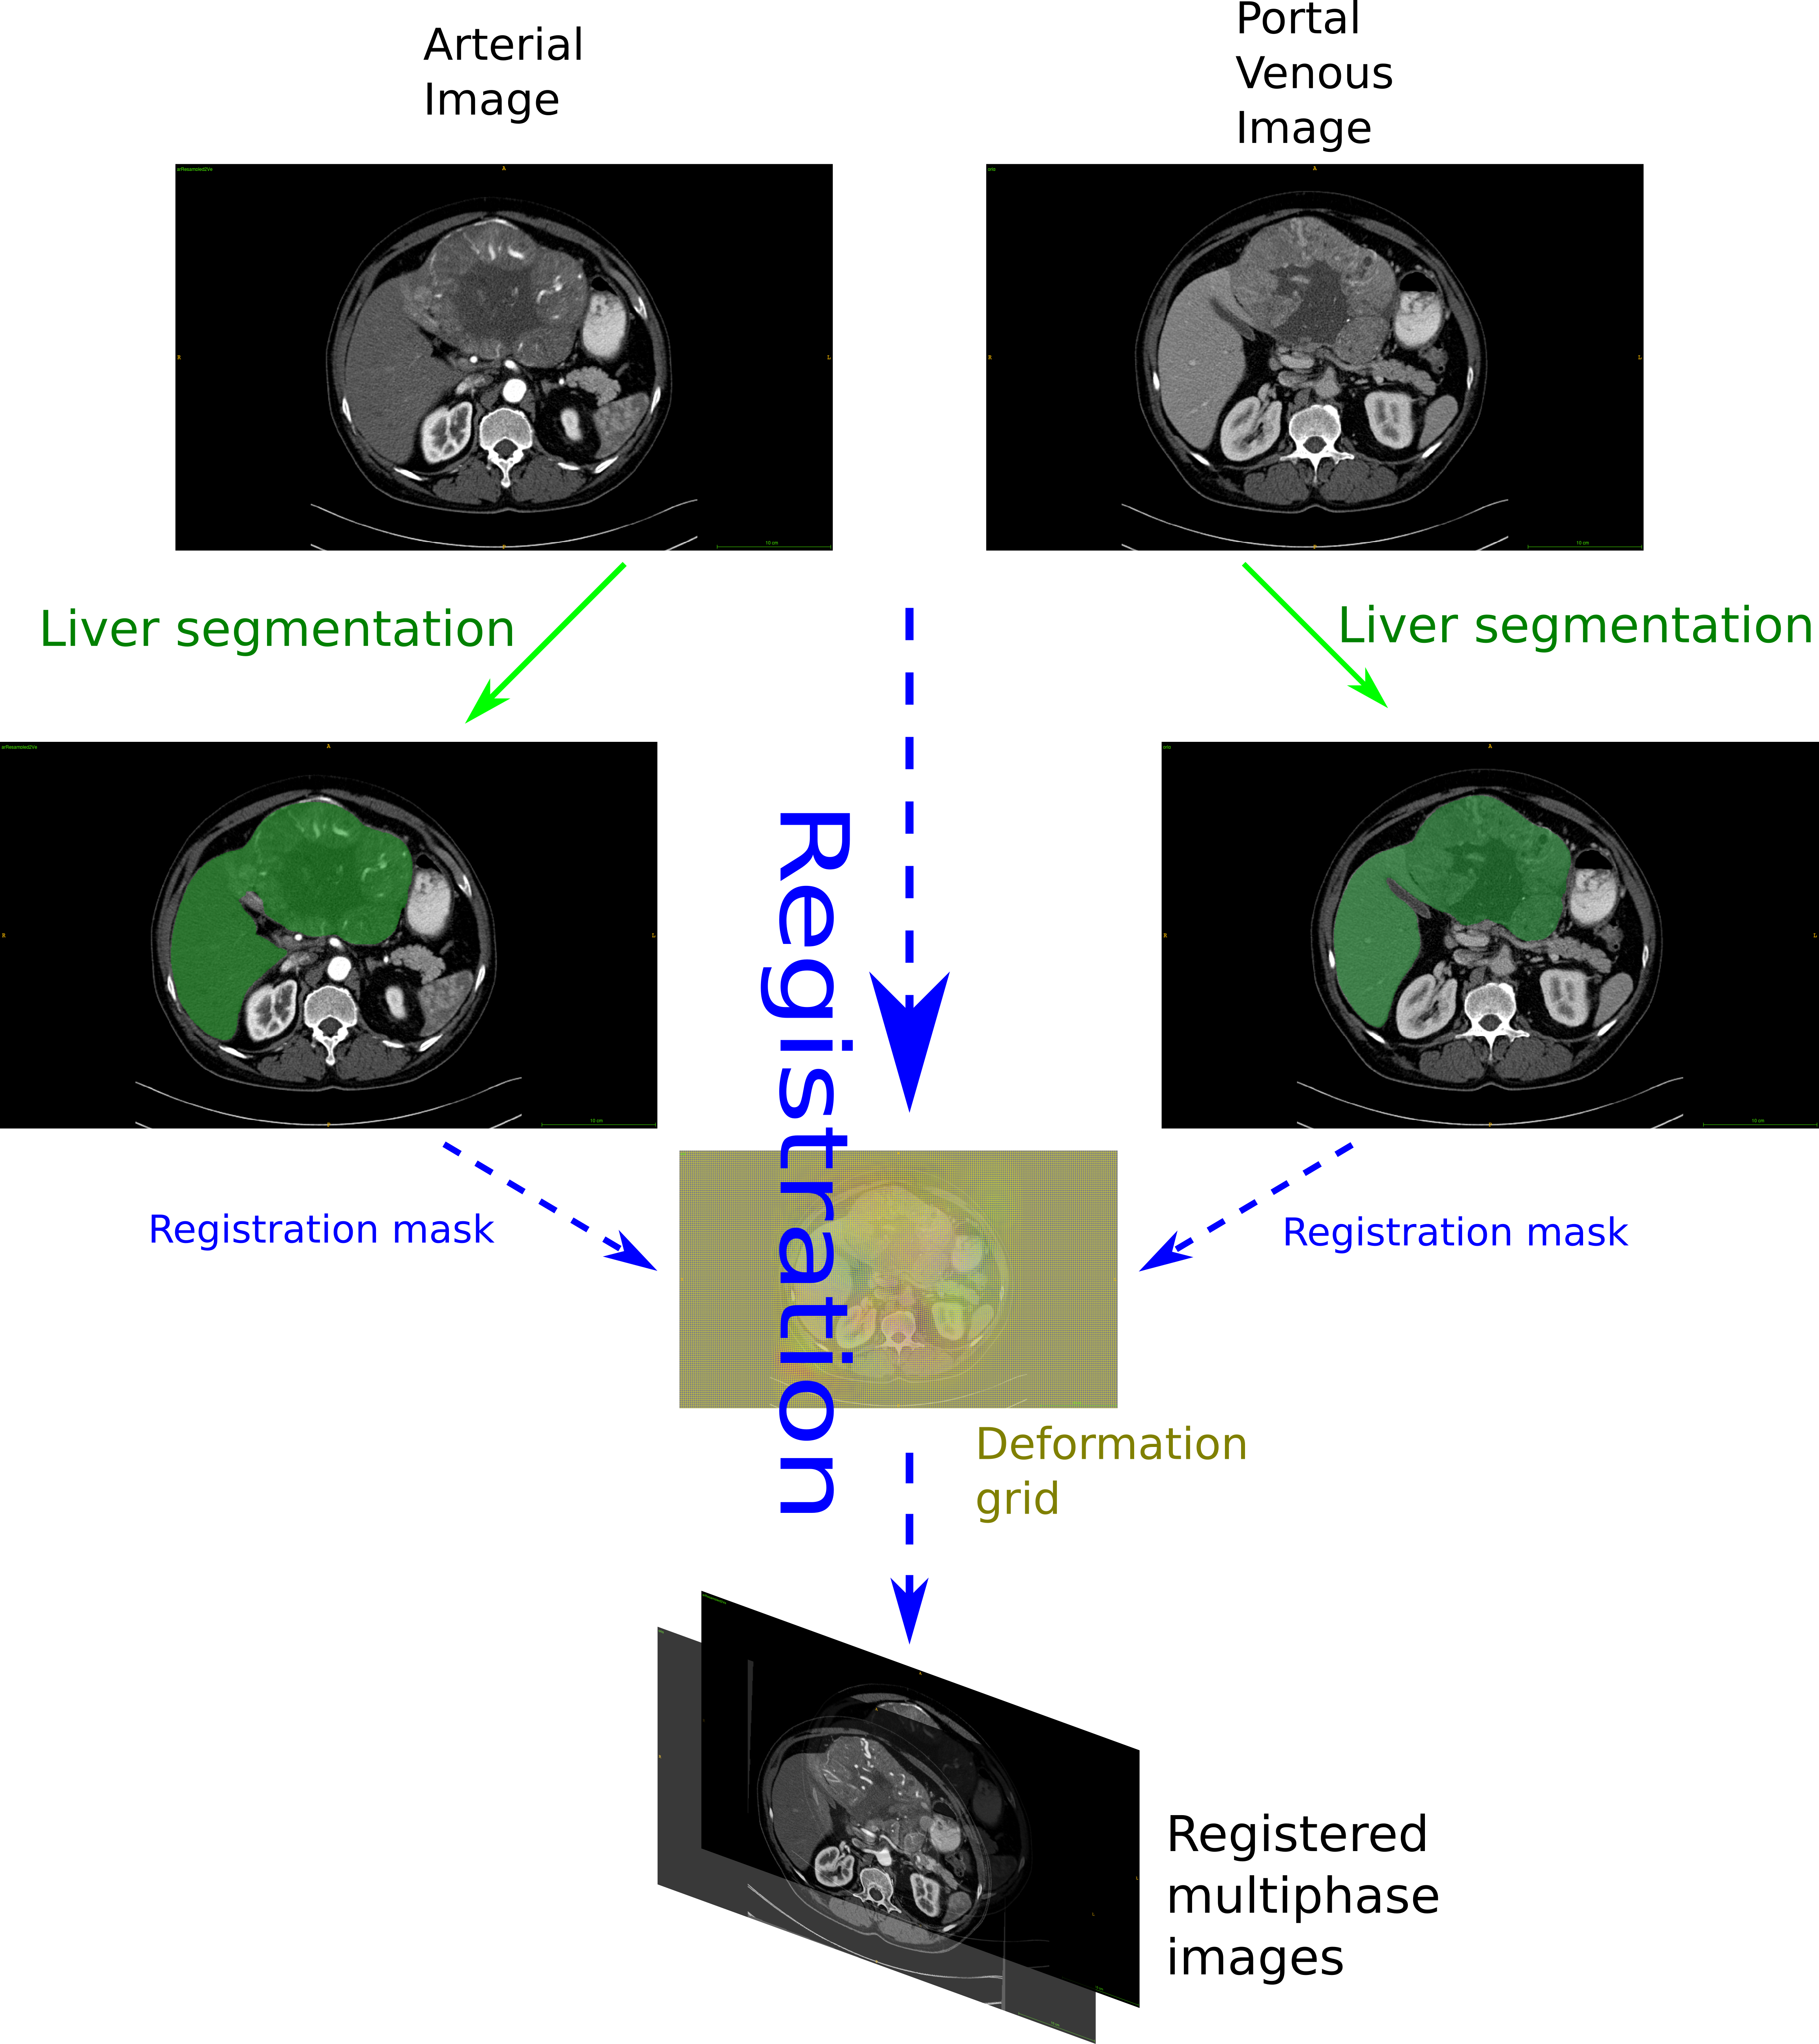
\includegraphics[width=0.7\linewidth]{../HistologicalGradePrediction/images/RegistrationTCIA_pipeline_vertical2}
\caption{Illustration of the registration pipeline applied to the images of \textbf{\lmttfont{TCIA-dB}}. The first green arrows correspond to the liver segmentation using a network trained on the \textbf{\lmttfont{LITS-dB}}. Dashed blue arrows correspond to the ANTs registration pipeline, where a dilated version of the predicted liver annotations maps are used as registration masks. The ANTs algorithm implements 3 transformations: a rigid, an affine, and a diffeomorphic Syn transformation that computes a deformation grid \cite{Avants2008}. The 3 steps of the ANTs algorithm allows us to obtain registered multiphase images.}
\label{fig:RegistrationTCIA_pipeline_vertical2}
\end{figure}


One way to perform a registration is to implement a series of
transformations (rigid or non-rigid) that will match a moving volume to
a target one. Each step of the registration is controlled by a
similarity loss.
When dealing with \ac{ct} volumes the available losses controlling the
different steps of the registration pipeline can be affected by areas of
the body with a high gradient such as the bones for example. When
registering two \ac{ct} volumes, one can either directly use both the entire
volumes or constraints the registration to a specific area (aka mask).
The liver being a soft organ, it easily moves with the respiratory
motions, in order to reduce the effect of the neighboring parts of the
abdomen, we have decided to restrict the computation of the similarity
metrics to the dilated liver mask area so that the registration
algorithm mainly focuses on the gradient present along its borders.

Consequently, the first step for the \textbf{\lmttfont{TCIA-dB}} registration is to perform a
liver semantic segmentation (green arrows in the figure \ref{fig:RegistrationTCIA_pipeline_vertical2}).

\subsection{Automatic liver segmentation}\label{tcia-db-unsupervised-liver-segmentation}

\subsubsection{Material}\label{tcia-db-unsupervised-liver-segmentation_material}
\textcolor{red}{Our objective is to automatically segment the liver on both the \ac{ar} and the \ac{pv} phased volumes of the \textbf{\lmttfont{TCIA-dB}}.}
In the available datasets (as presented in the table \ref{xp_datasets}), only \textbf{\lmttfont{TheraHCC-dB}} and \textbf{\lmttfont{LITS-dB}} contained expert liver delineation.
\textbf{\lmttfont{TheraHCC-dB}} contains annotations only on sparse slices across the liver,
whereas \textbf{\lmttfont{LITS-dB}} contains full 3D pixel-wise liver annotation but it only
contains single-phase images, without any information regarding the
acquisition phase (\ac{ar}, \ac{pv} and potentially DELAY volumes are mixed in the dataset).
\textcolor{red}
{
Regarding its design and the high number of segmented cases it contained, we decided to train our liver segmentation network on the \textbf{\lmttfont{LITS-dB}} volumes and test it on \textbf{\lmttfont{TCIA-dB}} patients.
We inspected both datasets to assess if a network trained on the \textbf{\lmttfont{LITS-dB}} volumes could perform the wanted task. Therefore, a medical expert was asked to determinate the differences between the two datasets with a visual examination of the CT volumes and through a quantitative analysis of the HU intensities after placement of ROIs.
For the visual examination, the medical expert was asked to list the different type of features present in both datasets.
They both contained liver volumes affected by large solitary tumors (HCC-like lesions), but some other smaller solitary tumors have also been found in both datasets, as depicted in the figure \ref{fig:interdb_tumorExamples}. 
\begin{figure}[!ht]
	\begin{mdframed}[backgroundcolor=blue!50,linecolor=blue!50]
		\centering
		\begin{minipage}{0.45\linewidth}
			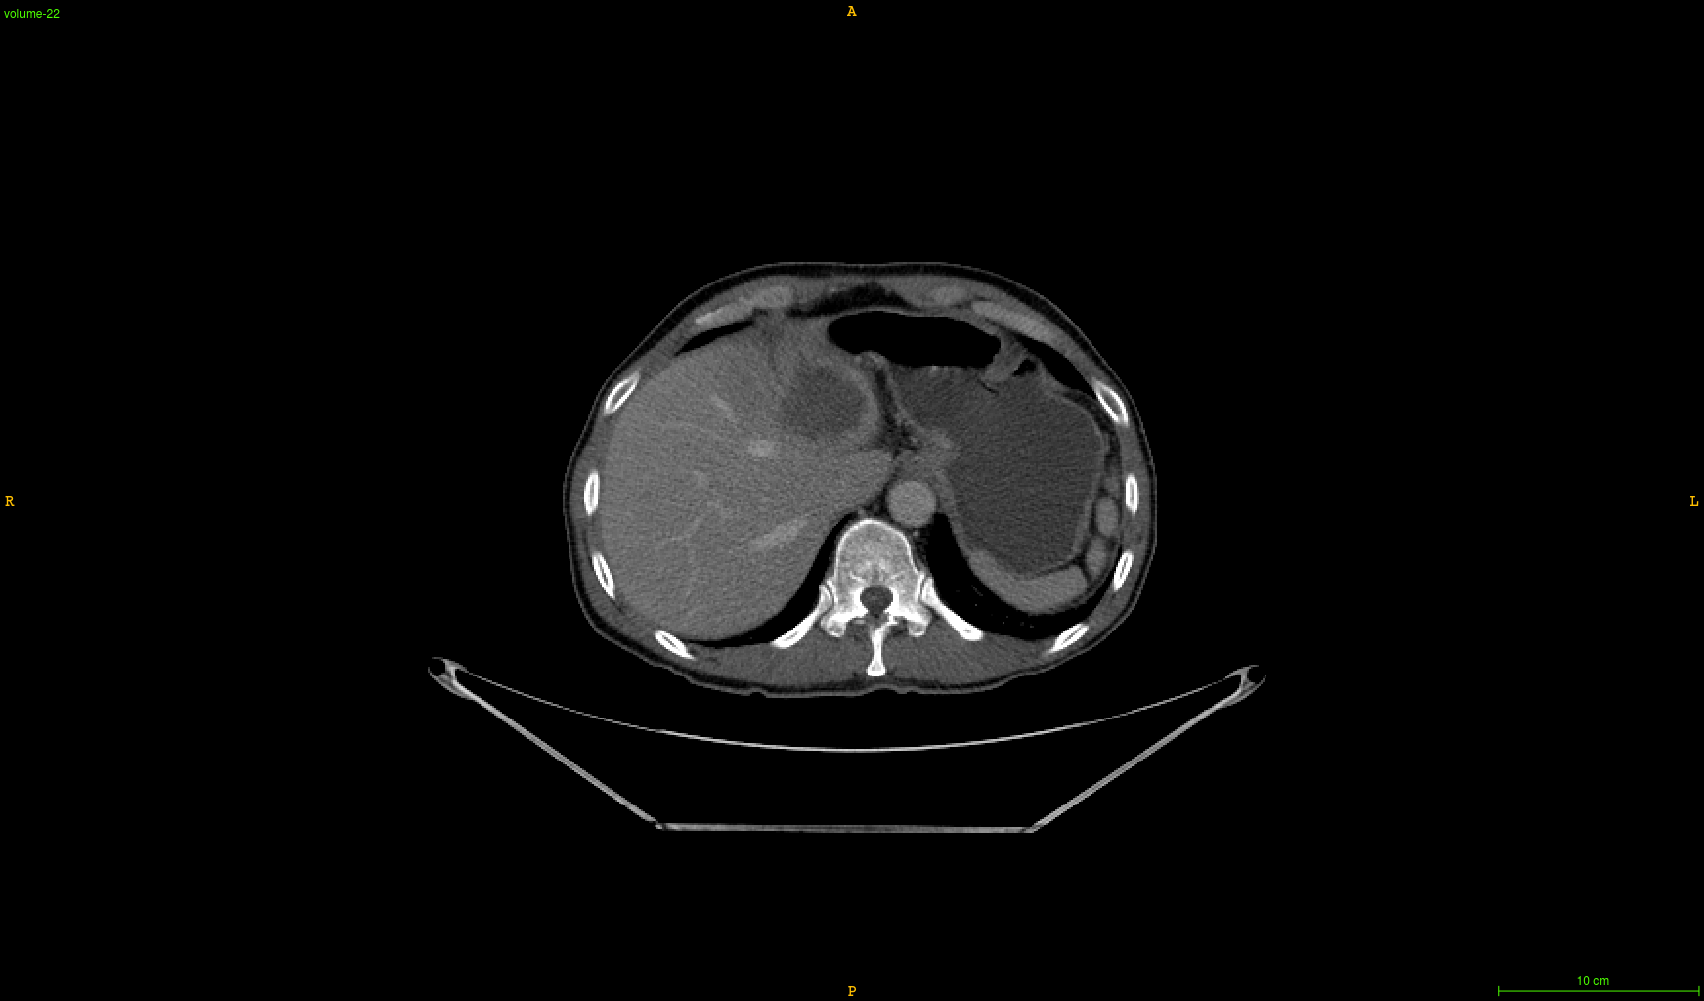
\includegraphics[width=\linewidth]{images/LITS_examplePatientSmallTumor_2}
		\end{minipage} \hspace{-0.1cm}
		\begin{minipage}{0.45\linewidth}
			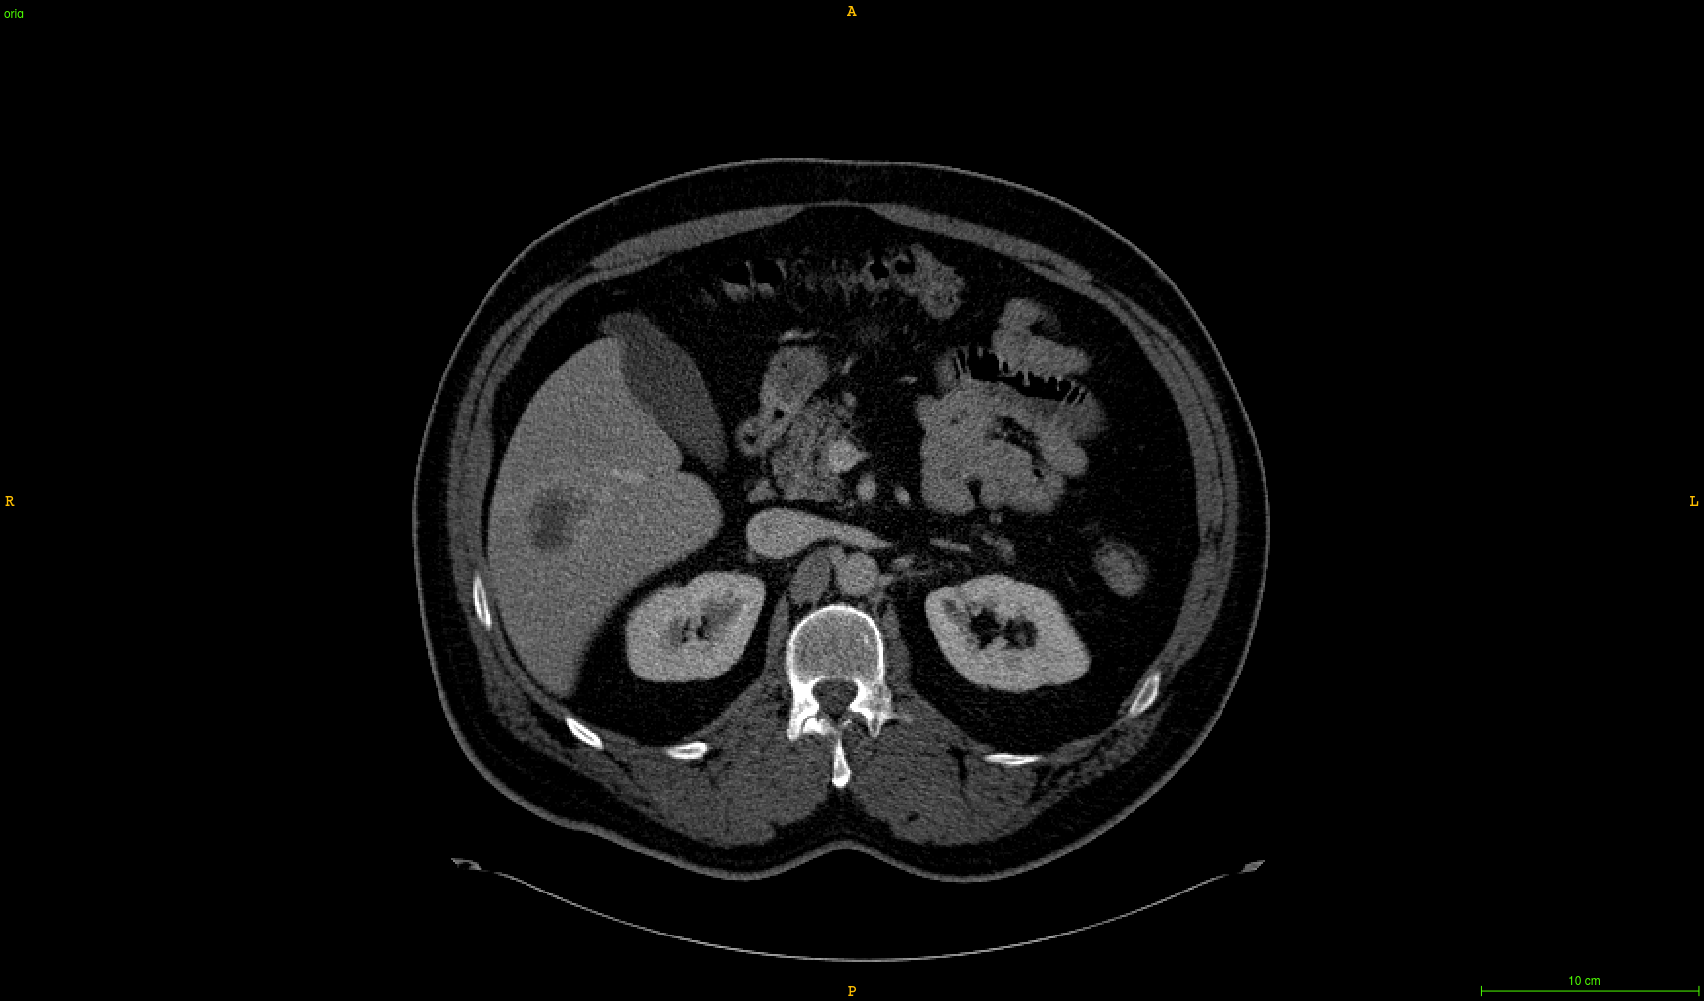
\includegraphics[width=\linewidth]{images/TCIA_examplePatientSmallTumor}
		\end{minipage} \\
		\begin{minipage}{0.45\linewidth}
			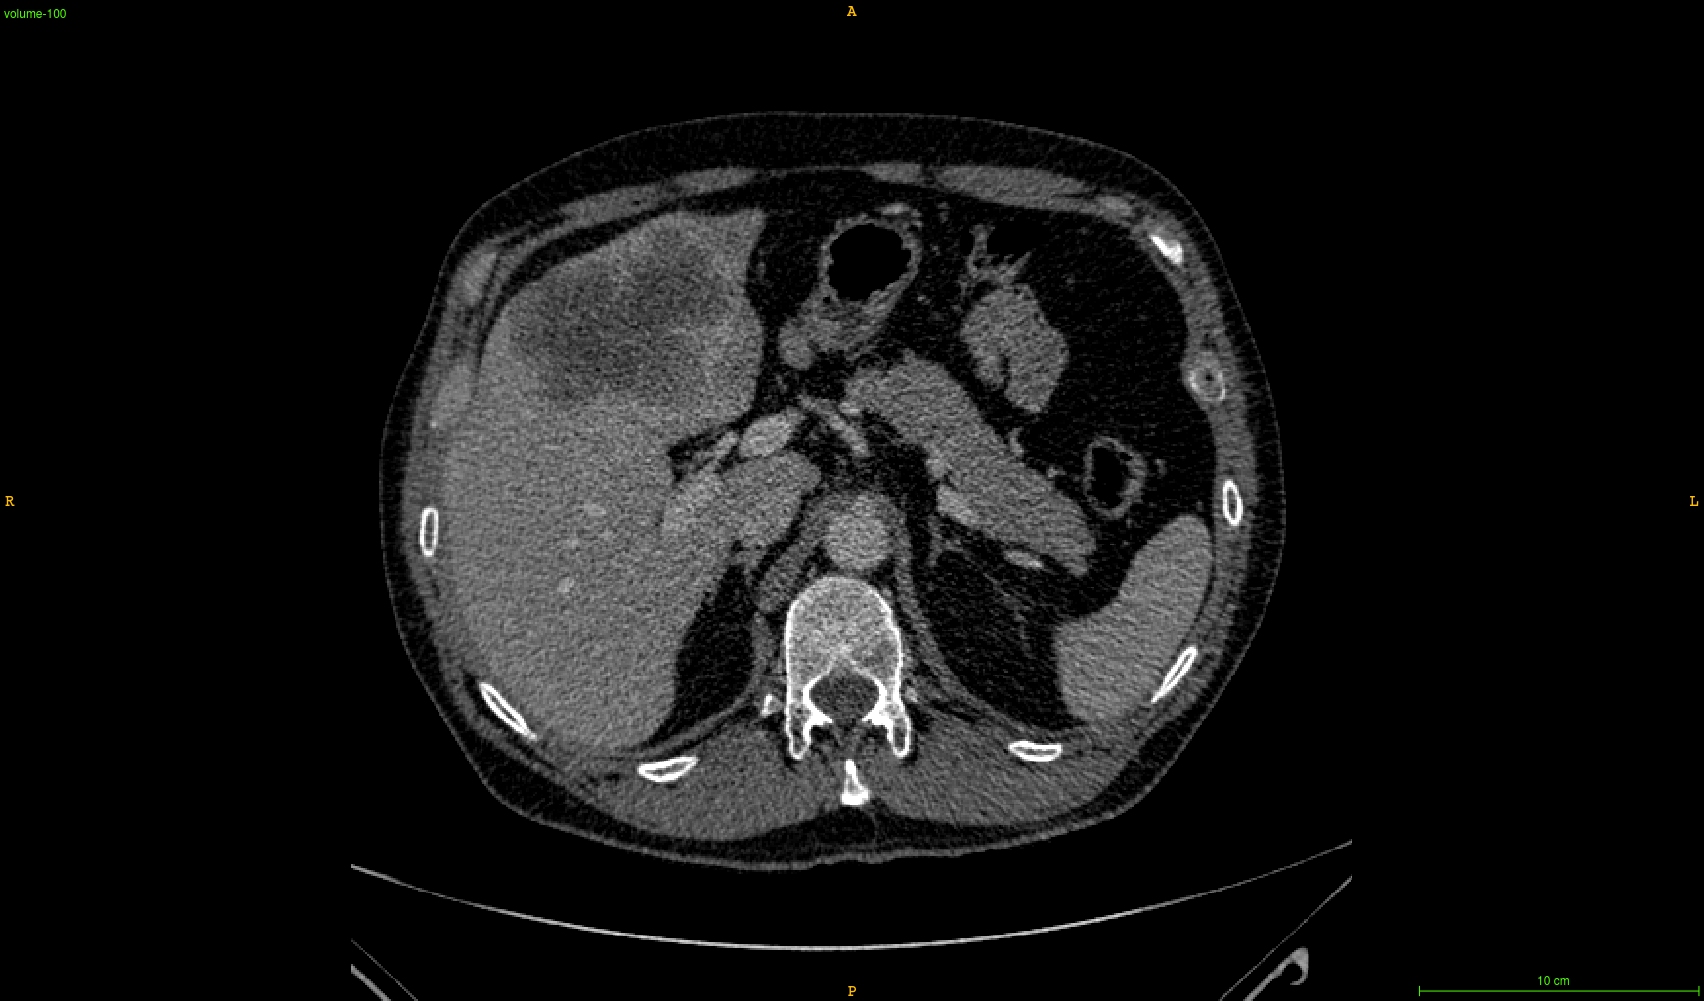
\includegraphics[width=\linewidth]{images/LITS_examplePatientLargeTumor}
		\end{minipage} \hspace{-0.1cm}
		\begin{minipage}{0.45\linewidth}
			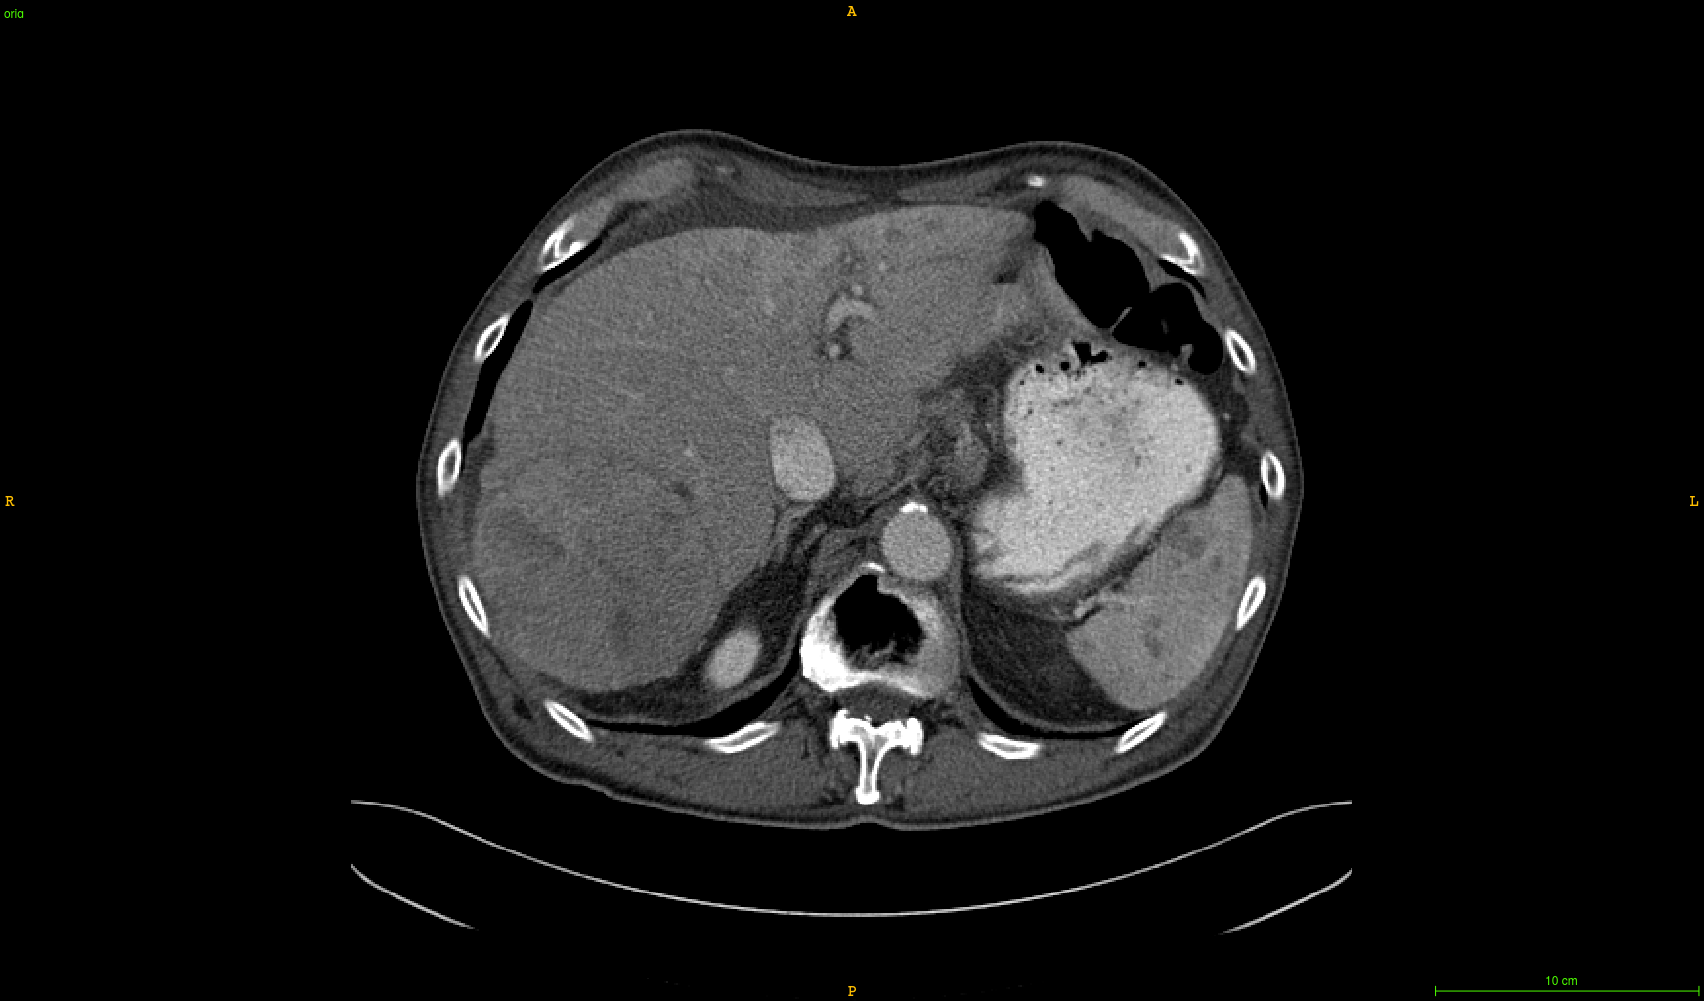
\includegraphics[width=\linewidth]{images/TCIA_examplePatientLargeTumor}
		\end{minipage}
	\end{mdframed}
	\caption{Example of small and large tumors from both the training and the testing datasets. Left: \textbf{\lmttfont{LITS-dB}} images, right: \textbf{\lmttfont{TCIA-dB}} images, top: small tumors, bottom: large tumors.}
	\label{fig:interdb_tumorExamples}
\end{figure}
It is worth noting that only the \textbf{\lmttfont{LITS-dB}} contained volumes with multiple lesions suspected to be metastases, as illustrated in the figure \ref{fig:litsDb_meta}.
\begin{figure}[!ht]
	\begin{mdframed}[backgroundcolor=blue!50,linecolor=blue!50]
		\centering
		\begin{minipage}{0.45\linewidth}
			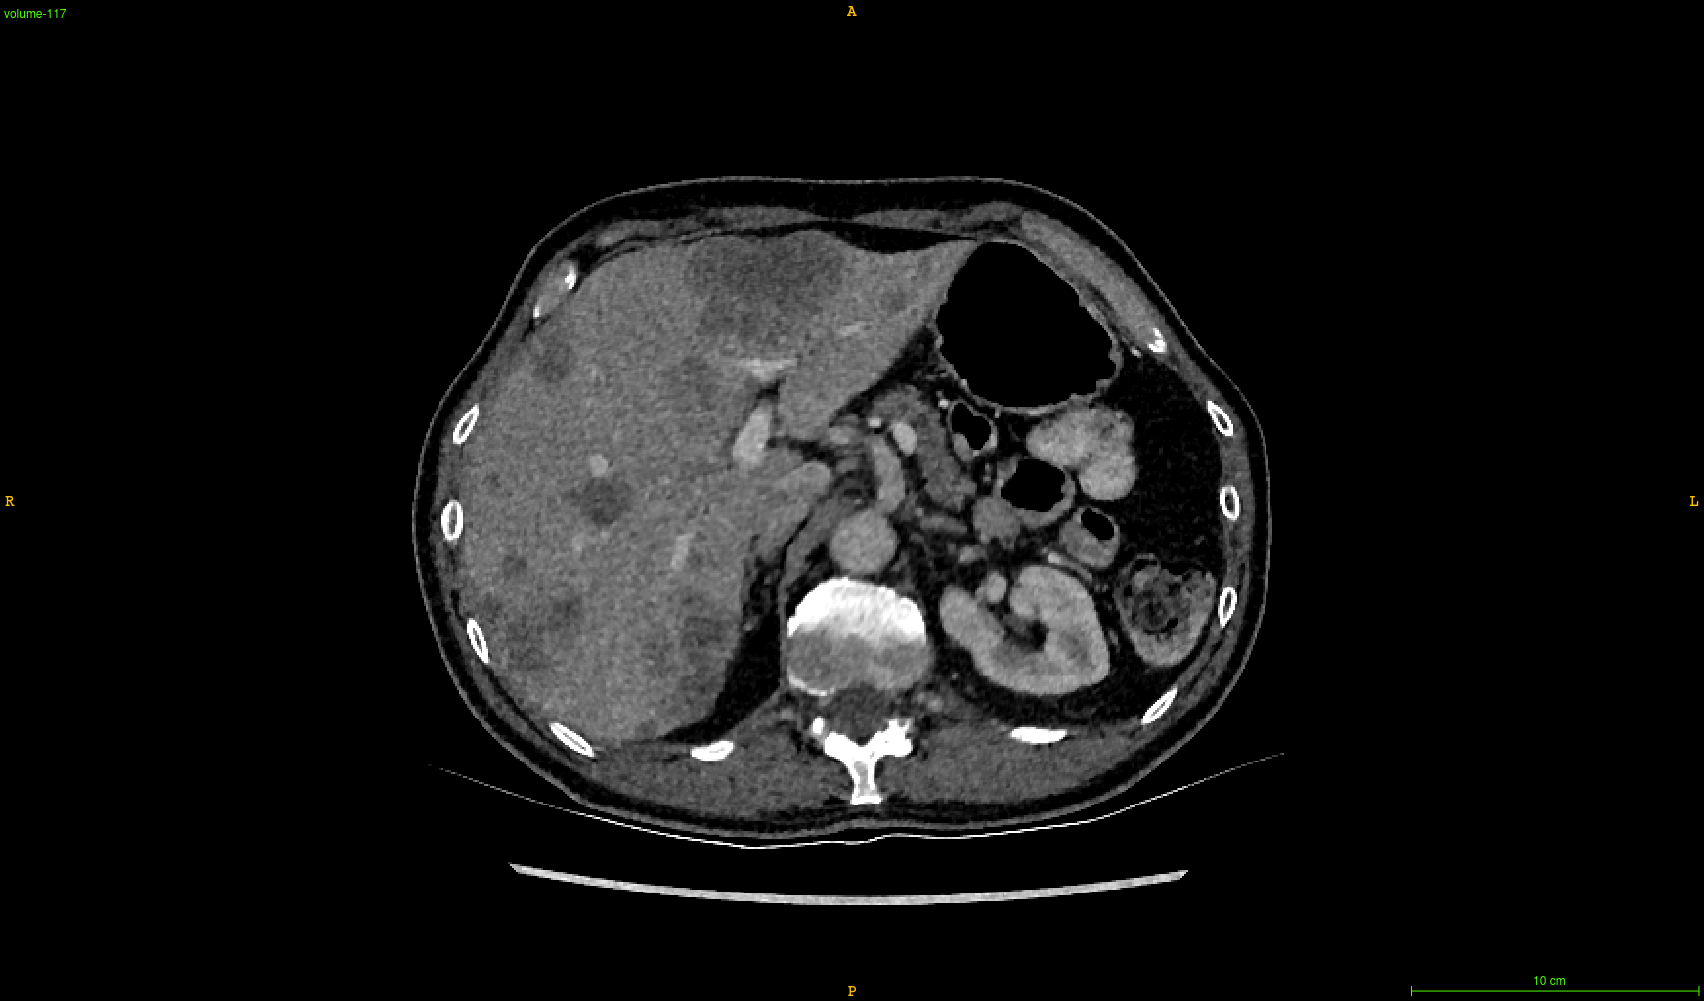
\includegraphics[width=\linewidth]{images/LITS_examplePatientMeta}
		\end{minipage} \hspace{-0.1cm}
		\begin{minipage}{0.45\linewidth}
			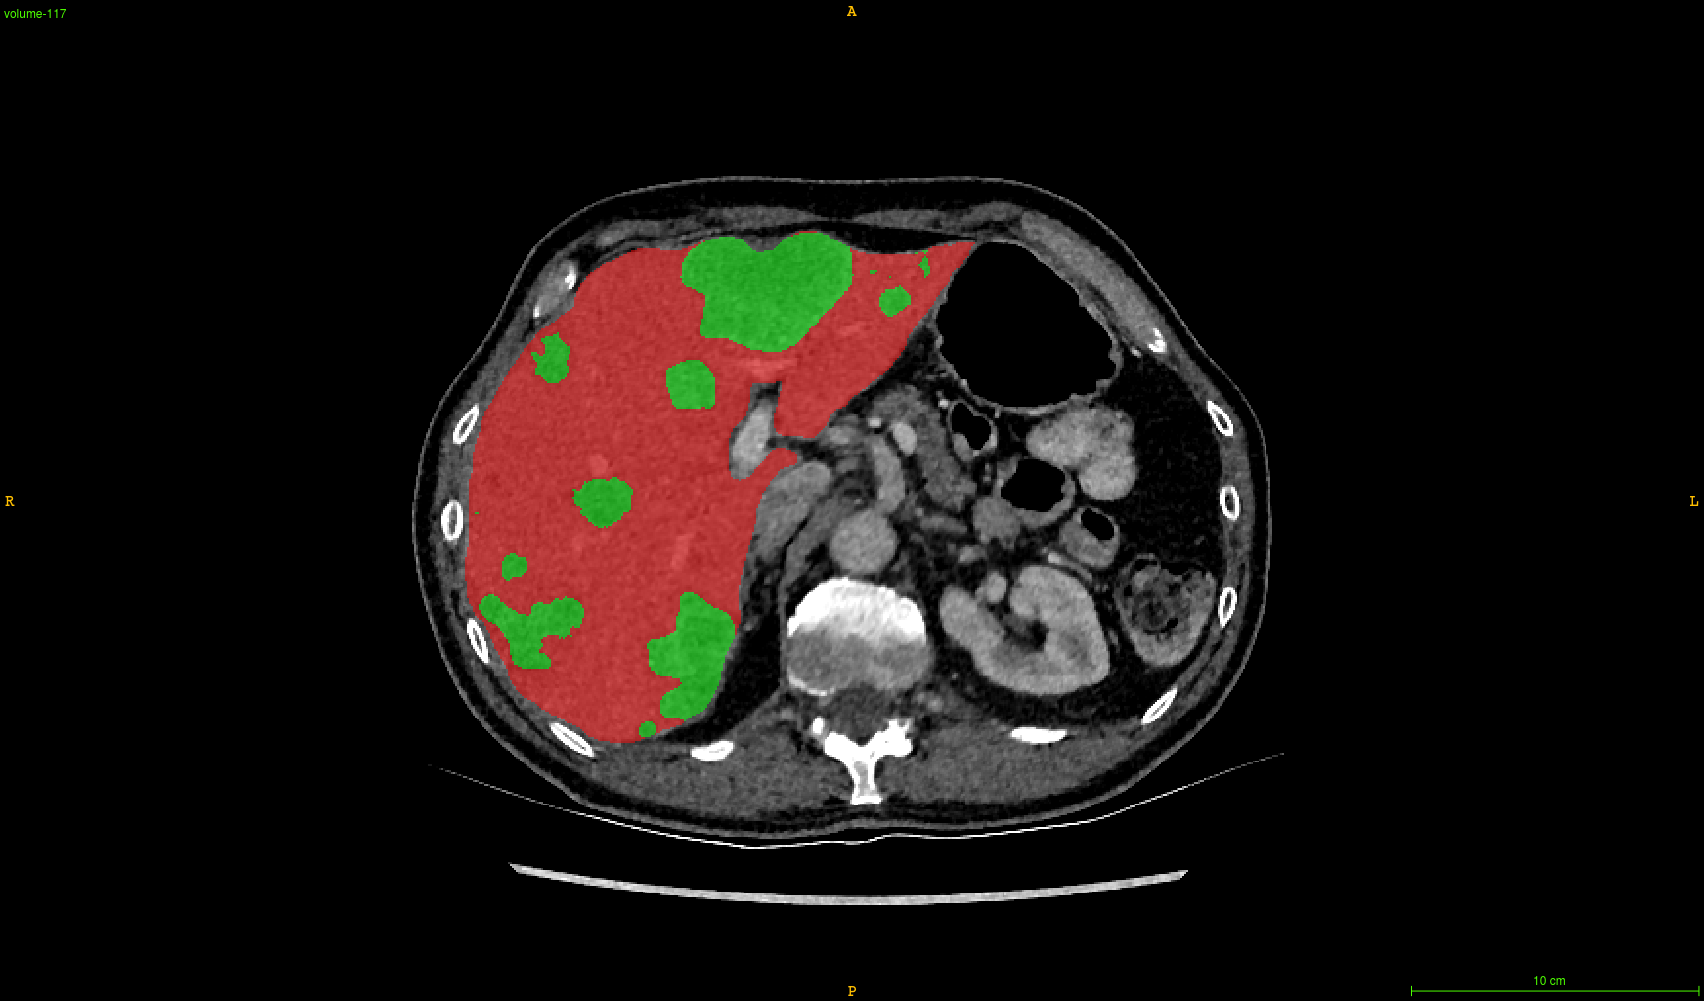
\includegraphics[width=\linewidth]{images/LITS_examplePatientMeta_seg}
		\end{minipage}
	\end{mdframed}
	\caption{Example of patient from the \textbf{\lmttfont{LITS-dB}} with a high number of tumors susceptible of being metastases. Right : raw image, left: expert segmentation where red represents liver parenchyma and green represents tumors.}
	\label{fig:litsDb_meta}
\end{figure}
Both datasets presented livers with benign lesions, track of fat deposit, or other metallic artifacts, as illustrated in the figure \ref{fig:InterDb_artifacts}.
\begin{figure}[!ht]
	\begin{mdframed}[backgroundcolor=blue!50,linecolor=blue!50]
		\centering
		\begin{minipage}{0.45\linewidth}
			\includegraphics[width=\linewidth]{images/Artifacts/LITS_cyst}
		\end{minipage} \hspace{-0.1cm}
		\begin{minipage}{0.45\linewidth}
			\includegraphics[width=\linewidth]{images/Artifacts/TCIA_cyst}
		\end{minipage} \\
		\begin{minipage}{0.45\linewidth}
			\includegraphics[width=\linewidth]{images/Artifacts/LITS_fat}
		\end{minipage} \hspace{-0.1cm}
		\begin{minipage}{0.45\linewidth}
			\includegraphics[width=\linewidth]{images/Artifacts/TCIA_fat}
		\end{minipage} \\
		\begin{minipage}{0.45\linewidth}
			\includegraphics[width=\linewidth]{images/Artifacts/LITS_metallic_artifacts}
		\end{minipage} \hspace{-0.1cm}
		\begin{minipage}{0.45\linewidth}
			\includegraphics[width=\linewidth]{images/Artifacts/TCIA_metallic_artifacts}
		\end{minipage}
	\end{mdframed}
	\caption{Example of artifacts present in both training and test datasets. Left: \textbf{\lmttfont{LITS-dB}} images, right: \textbf{\lmttfont{TCIA-dB}} images. First row presents patients with benign hepatic lesions (yellow arrows), second row presents liver with tracks of fat accumulation (orange arrows), whereas last row gives examples of images with presence of metallic artifacts (red arrows).}
	\label{fig:InterDb_artifacts}
\end{figure}
Diseased livers were also present in both datasets, where severe signs of cirrhosis were noticed, as exposed in the figure \ref{fig:InterDb_diseasedLivers}.
\begin{figure}[!ht]
	\begin{mdframed}[backgroundcolor=blue!50,linecolor=blue!50]
		\centering
		\begin{minipage}{0.45\linewidth}
			\includegraphics[width=\linewidth]{images/LITS_cirrhoticPatientArrows}
		\end{minipage} \hspace{-0.1cm}
		\begin{minipage}{0.45\linewidth}
			\includegraphics[width=\linewidth]{images/TCIA_cirrhoticPatientArrows}
		\end{minipage}
	\end{mdframed}
	\caption{Example of cirrhotic patients present in both datasets.  Left: \textbf{\lmttfont{LITS-dB}} images, right: \textbf{\lmttfont{TCIA-dB}} images. We can see the irregular shape (cyan arrows) of the liver with signs of atrophy (pink arrows) in both cases.}
	\label{fig:InterDb_diseasedLivers}
\end{figure}
A quantitative analysis has been performed on randomly chosen patients, where 5 ROIs were placed by the medical expert in the liver parenchyma, the air, the spleen, the bone and the aorta. The aorta was chosen to analyze the changes in term of contrast agent concentration. The liver parenchyma and the spleen were also affected by the contrast agent diffusion, but they were mainly used to diagnose diseased patients since a difference of more than 18.5 HU between both areas at portal venous phase could be a sign of cirrhosis \textbf{ADD REF}. It is worth noting that the ROIs in the liver parenchyma were placed in the peripheral parts of the liver to avoid vessels. The bone and the air ROIs served as control since the air is supposed to have always the same intensity (-1000 HU independently of the acquisition parameters), while the calcium present in the bone renders the circulation ot the contrast agent difficult, and this ROI can be used as a way to compare the different phases. An example of annotation is given in the figure \ref{fig:roiPlacement}. \\
The quantitative analysis proved the probable presence of cirrhotic patients in both datasets, as depicted in the figure \ref{fig:cirrhosisPlot}.
\begin{figure}[!ht]
	\begin{mdframed}[backgroundcolor=blue!50,linecolor=blue!50]
		\centering
		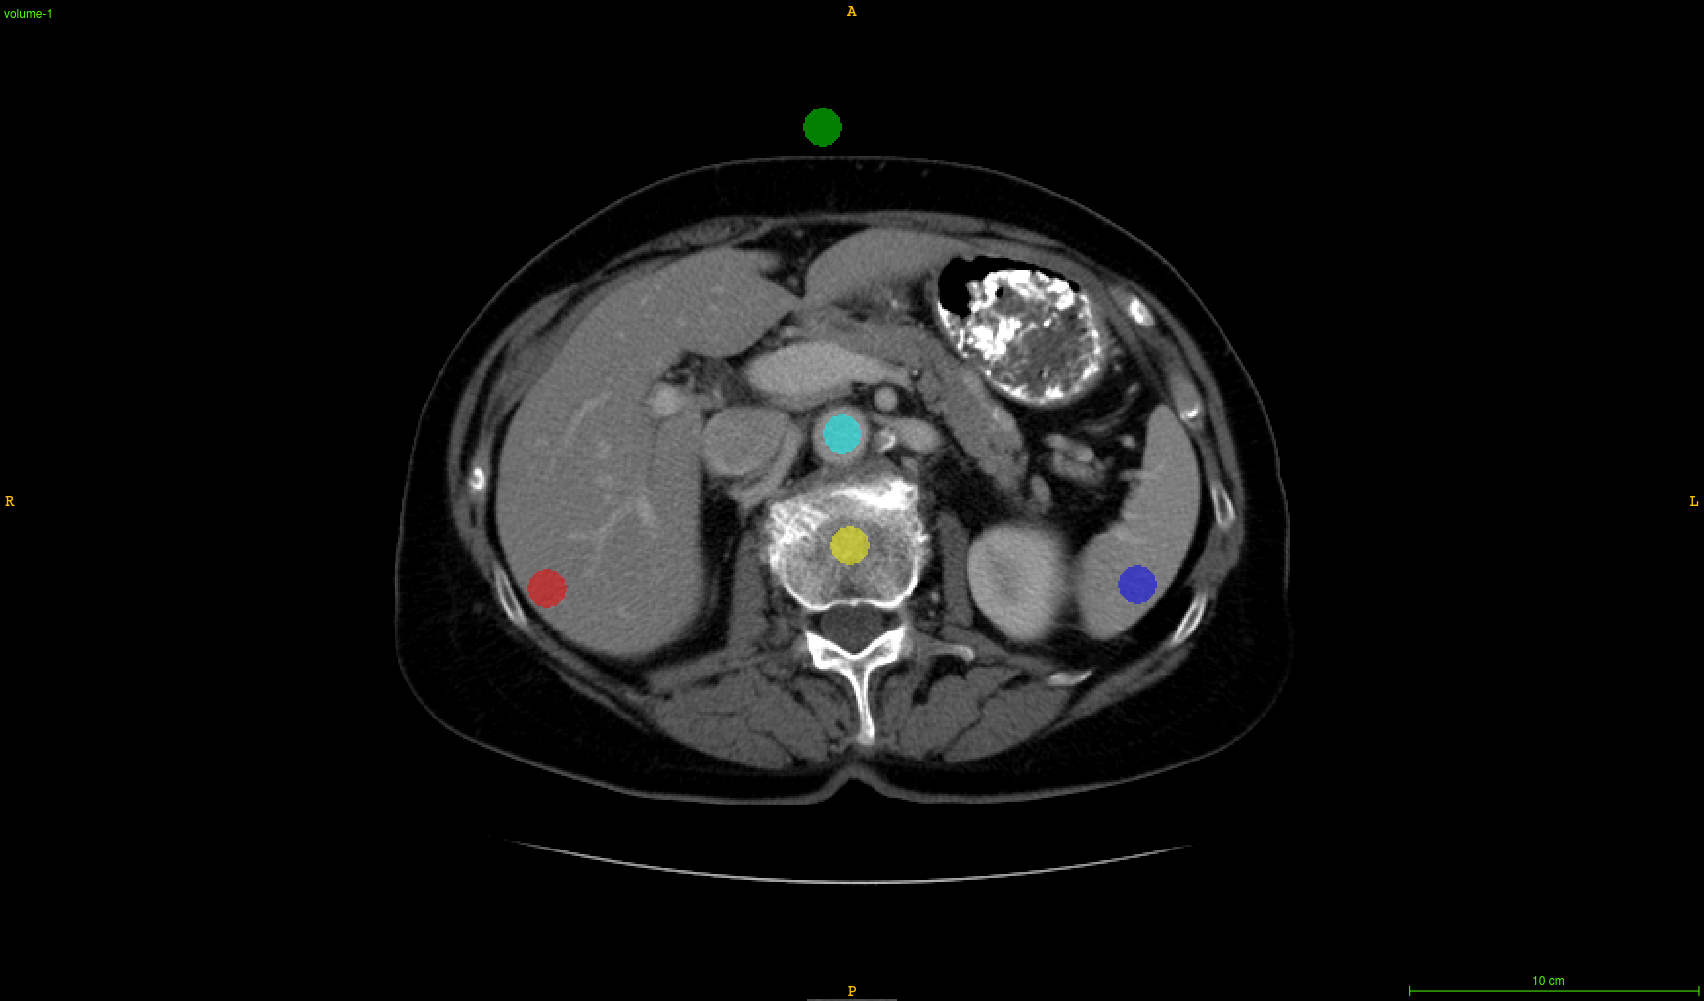
\includegraphics[width=0.6\linewidth]{images/juan_Roi_Example}
		\caption{Example of ROI placement for the quantitative evaluation of differences between the \textbf{\lmttfont{LITS-dB}} and the \textbf{\lmttfont{TCIA-dB}}. Red: liver parenchyma, green: air, blue: spleen, yellow: bone, cyan: aorta.}
		\label{fig:roiPlacement}
	\end{mdframed}
\end{figure}
\begin{figure}[!ht]
	\begin{mdframed}[backgroundcolor=blue!50,linecolor=blue!50]
		\centering
		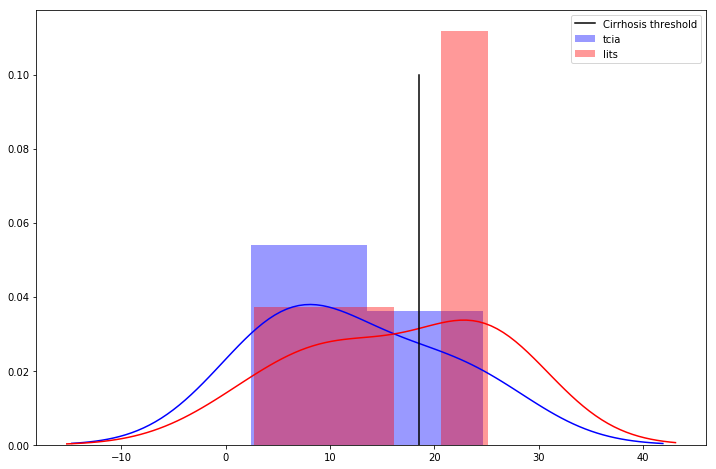
\includegraphics[width=0.6\linewidth]{images/LITS_TCIA_cirrhosisPlot}
		\caption{Histogram representing the distribution of the difference between parenchyma and spleen intensities, where a difference higher than 18.5 HU (black vertical line) can be a sign of cirrhosis.}
		\label{fig:cirrhosisPlot}
	\end{mdframed}
\end{figure}
Finally, regarding the available contrast-enhanced phases per dataset, it has been proved that \textbf{\lmttfont{LITS-dB}} contains volumes that can be labeled as arterial and some other that can be labeled as portal venous (see figure \ref{fig:LitsTciaPhasePlot}).
\begin{figure}[!ht]
	\begin{mdframed}[backgroundcolor=blue!50,linecolor=blue!50]
		\centering
		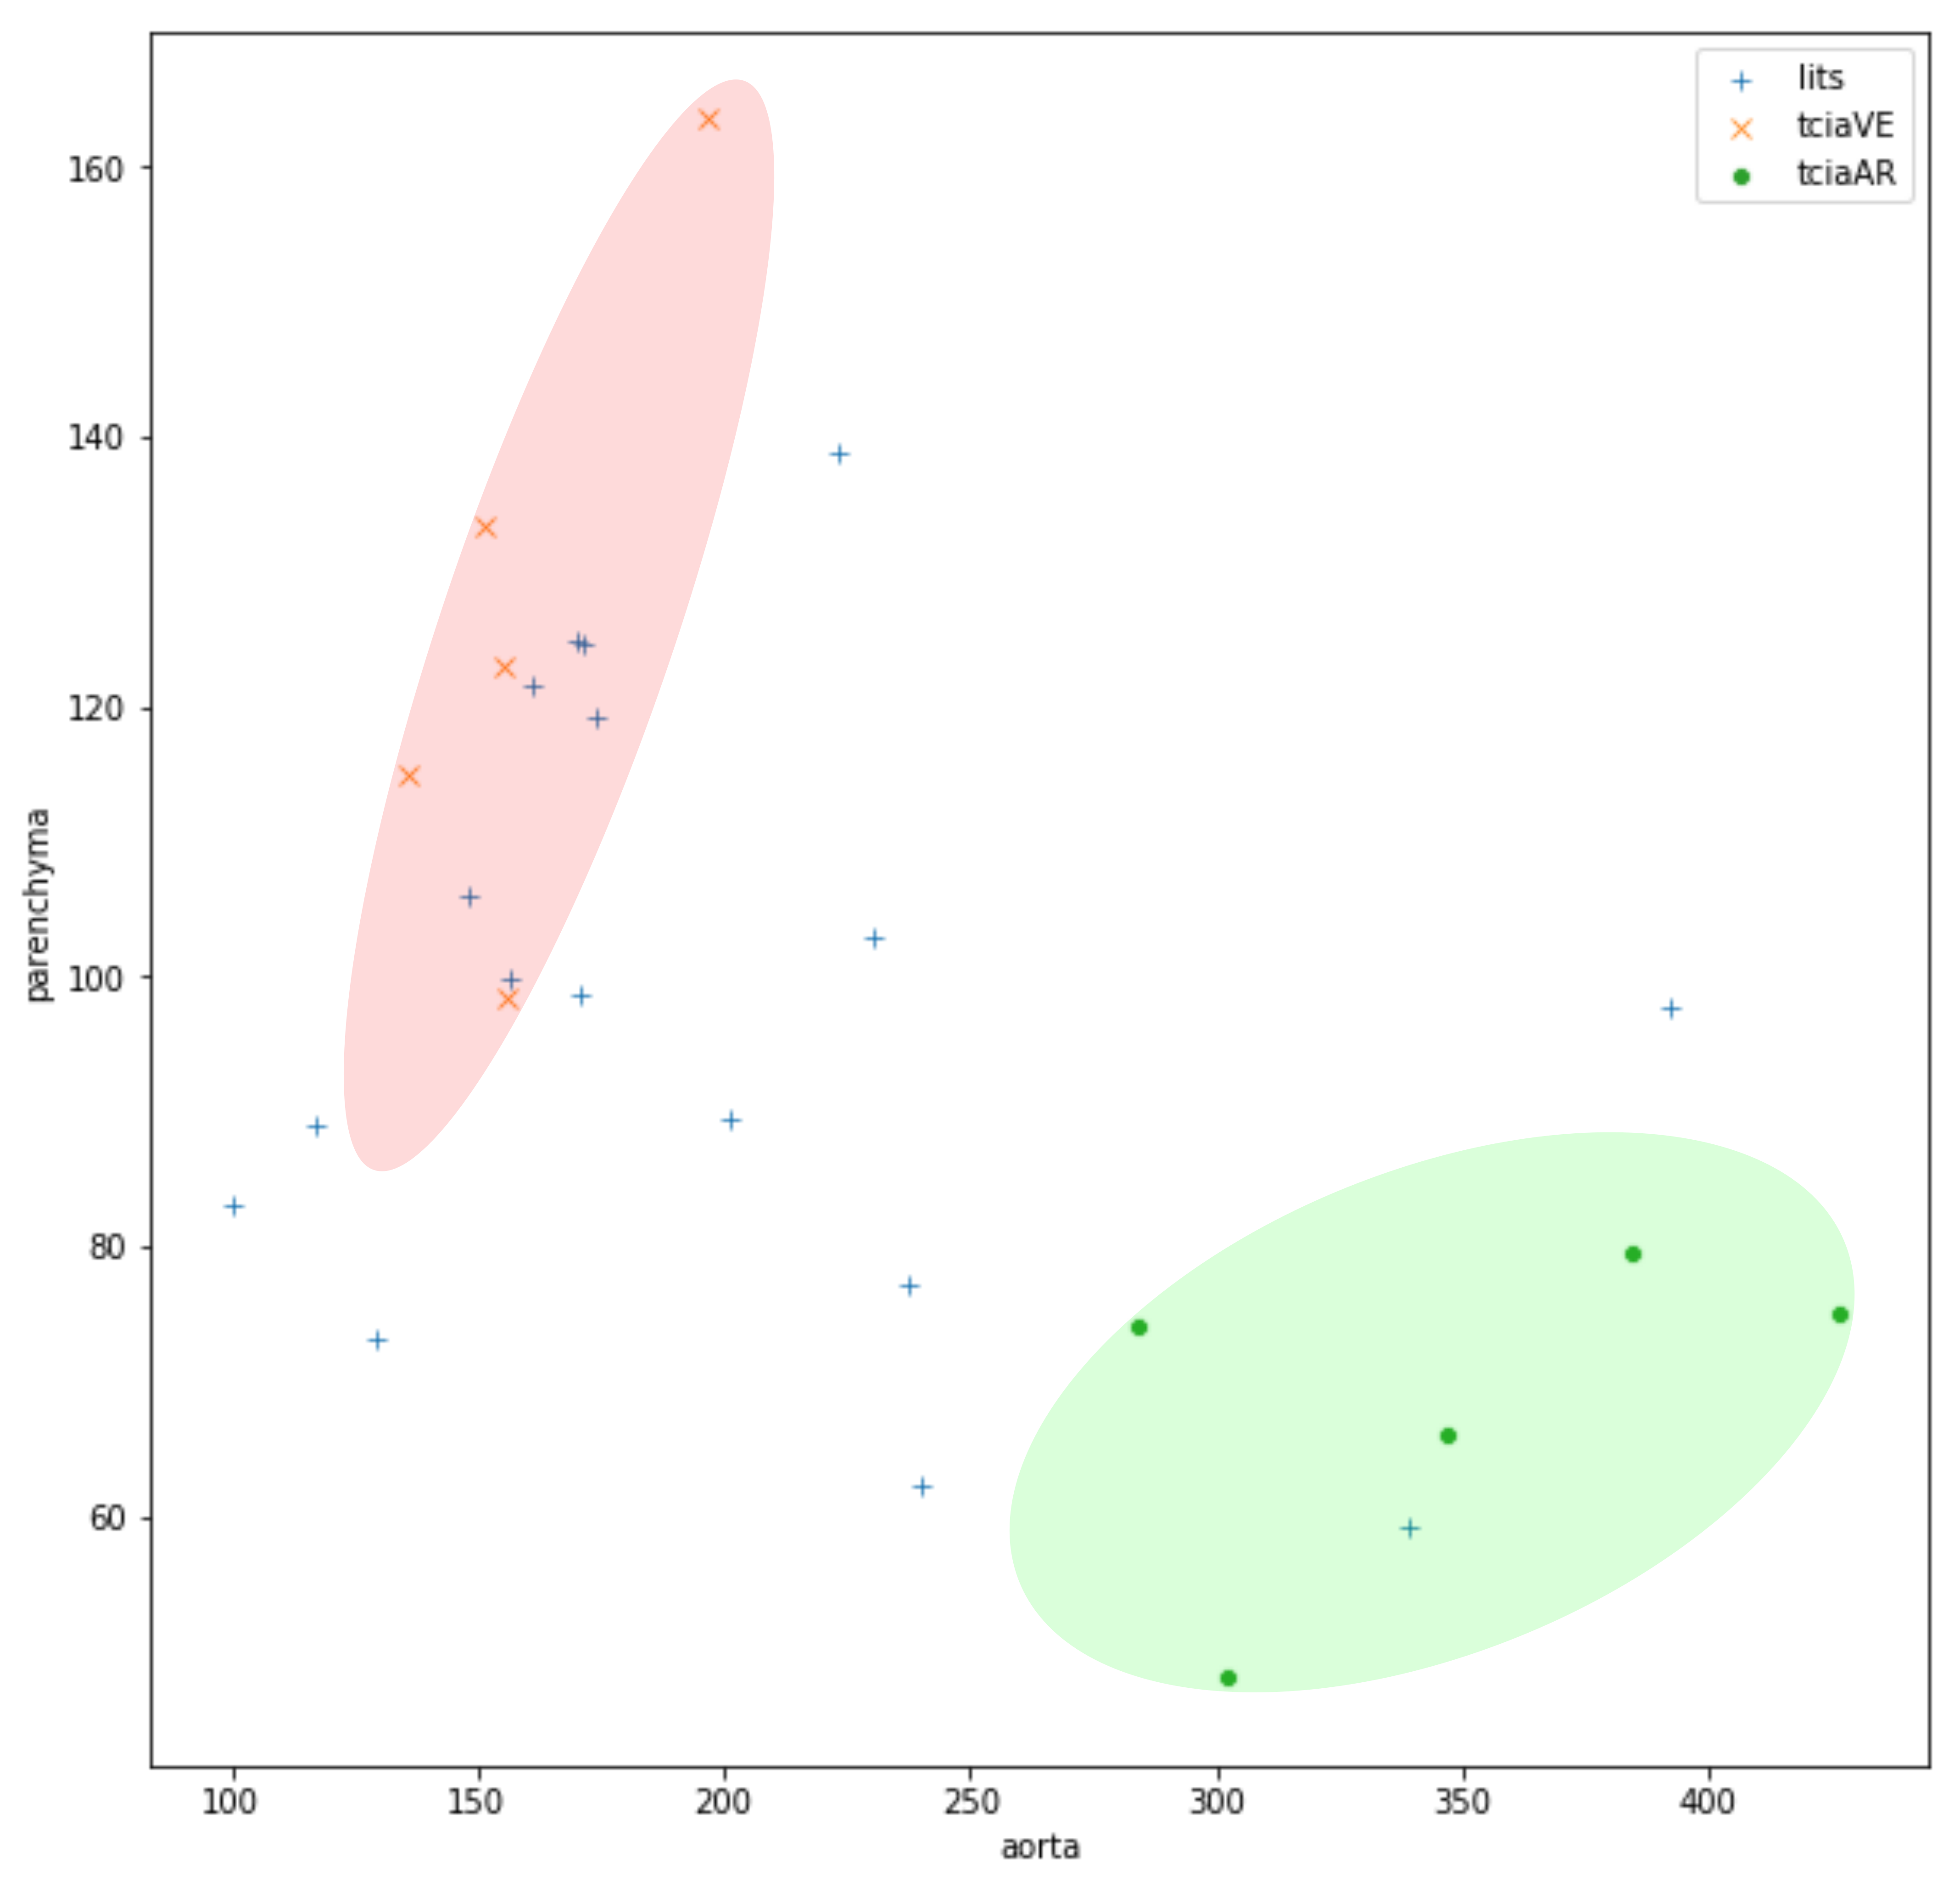
\includegraphics[width=0.6\linewidth]{images/AortaParPlot}
		\caption{Mean aorta intensity vs mean liver parenchyma intensity. Each point represents one volume. We can see a clear separation between arterial (green dots) and portal venous (red crosses) volumes among the \textbf{\lmttfont{TCIA-dB}} patients. Portal venous volumes present a higher variance for their liver parenchyma intensities, which can be explained by the differences in terms of duration between the injection of contrast medium and the acquisition of the images. It seems clear that the majority of volumes from the \textbf{\lmttfont{LITS-dB}} were acquired during the portal venous phase whereas some of them were acquired during the arterial phase. The rest of the volumes can be classified as belonging to the late arterial or the early portal venous phase.
		}
		\label{fig:LitsTciaPhasePlot}
	\end{mdframed}
\end{figure}
Since all the patients of the \textbf{\lmttfont{TCIA-dB}} were supposed to be affected by HCC, it would have been ideal to have a dataset only composed of patients suffering from HCC or by a large solitary tumor, but only 20 patients of the 131 from the \textbf{\lmttfont{LITS-dB}} were affected by a single lesion larger than $ 2cm^3 $.
Since we considered that the type of lesions will only slightly affect the liver segmentation, we decided to keep all the patients of the \textbf{\lmttfont{LITS-dB}} (independently of the number of lesions present in the liver) to train our liver segmentation network.
Moreover, it would have been optimal to train one network per injected phase, or a single network with multiphase images as input.
However \textbf{\lmttfont{TCIA-dB}} being the only available dataset with experts' liver segmentation, and since it is composed of both \ac{ar} and \ac{pv} volumes (with in-between phase volumes as depicted in the figure \ref{fig:LitsTciaPhasePlot}), we used the entire dataset to train a single network, allowing us to segment the liver on both \ac{ar} and \ac{pv} volumes independently.
}
%Our experiments however showed that a liver segmentation network trained
%on sufficiently enough cases is able to perform the semantic
%segmentation of both \ac{ar} and \ac{pv} raw images independently.

\subsubsection{Methods}\label{liver_segmentation_tcia_db_methods}

\textcolor{red}
{
We trained our network called \pplfont{\ac{cect}-Liver} on the 131 volumes of the
\textbf{\lmttfont{LITS-dB}} using the same hyperparameters as the ones detailed
previously. The network shares the same settings as the previously defined \pplfont{\ac{pv}-Liver} and \pplfont{\ac{ar}-Liver} networks, as detailed in the figure \ref{fig:CECTliverDetails}. In this case we used the architecture with 1024 filters at bottleneck, corresponding to about 32M parameters. Once the segmentation performed on each of the axial slices of a given patient, we implemented 2 post-processing steps by first extracting the biggest connected component in the entire 3D volume before applying a binary opening operation to the retained mask.
\begin{figure}[!ht]
	\begin{mdframed}[backgroundcolor=blue!50,linecolor=blue!50]
		\centering
		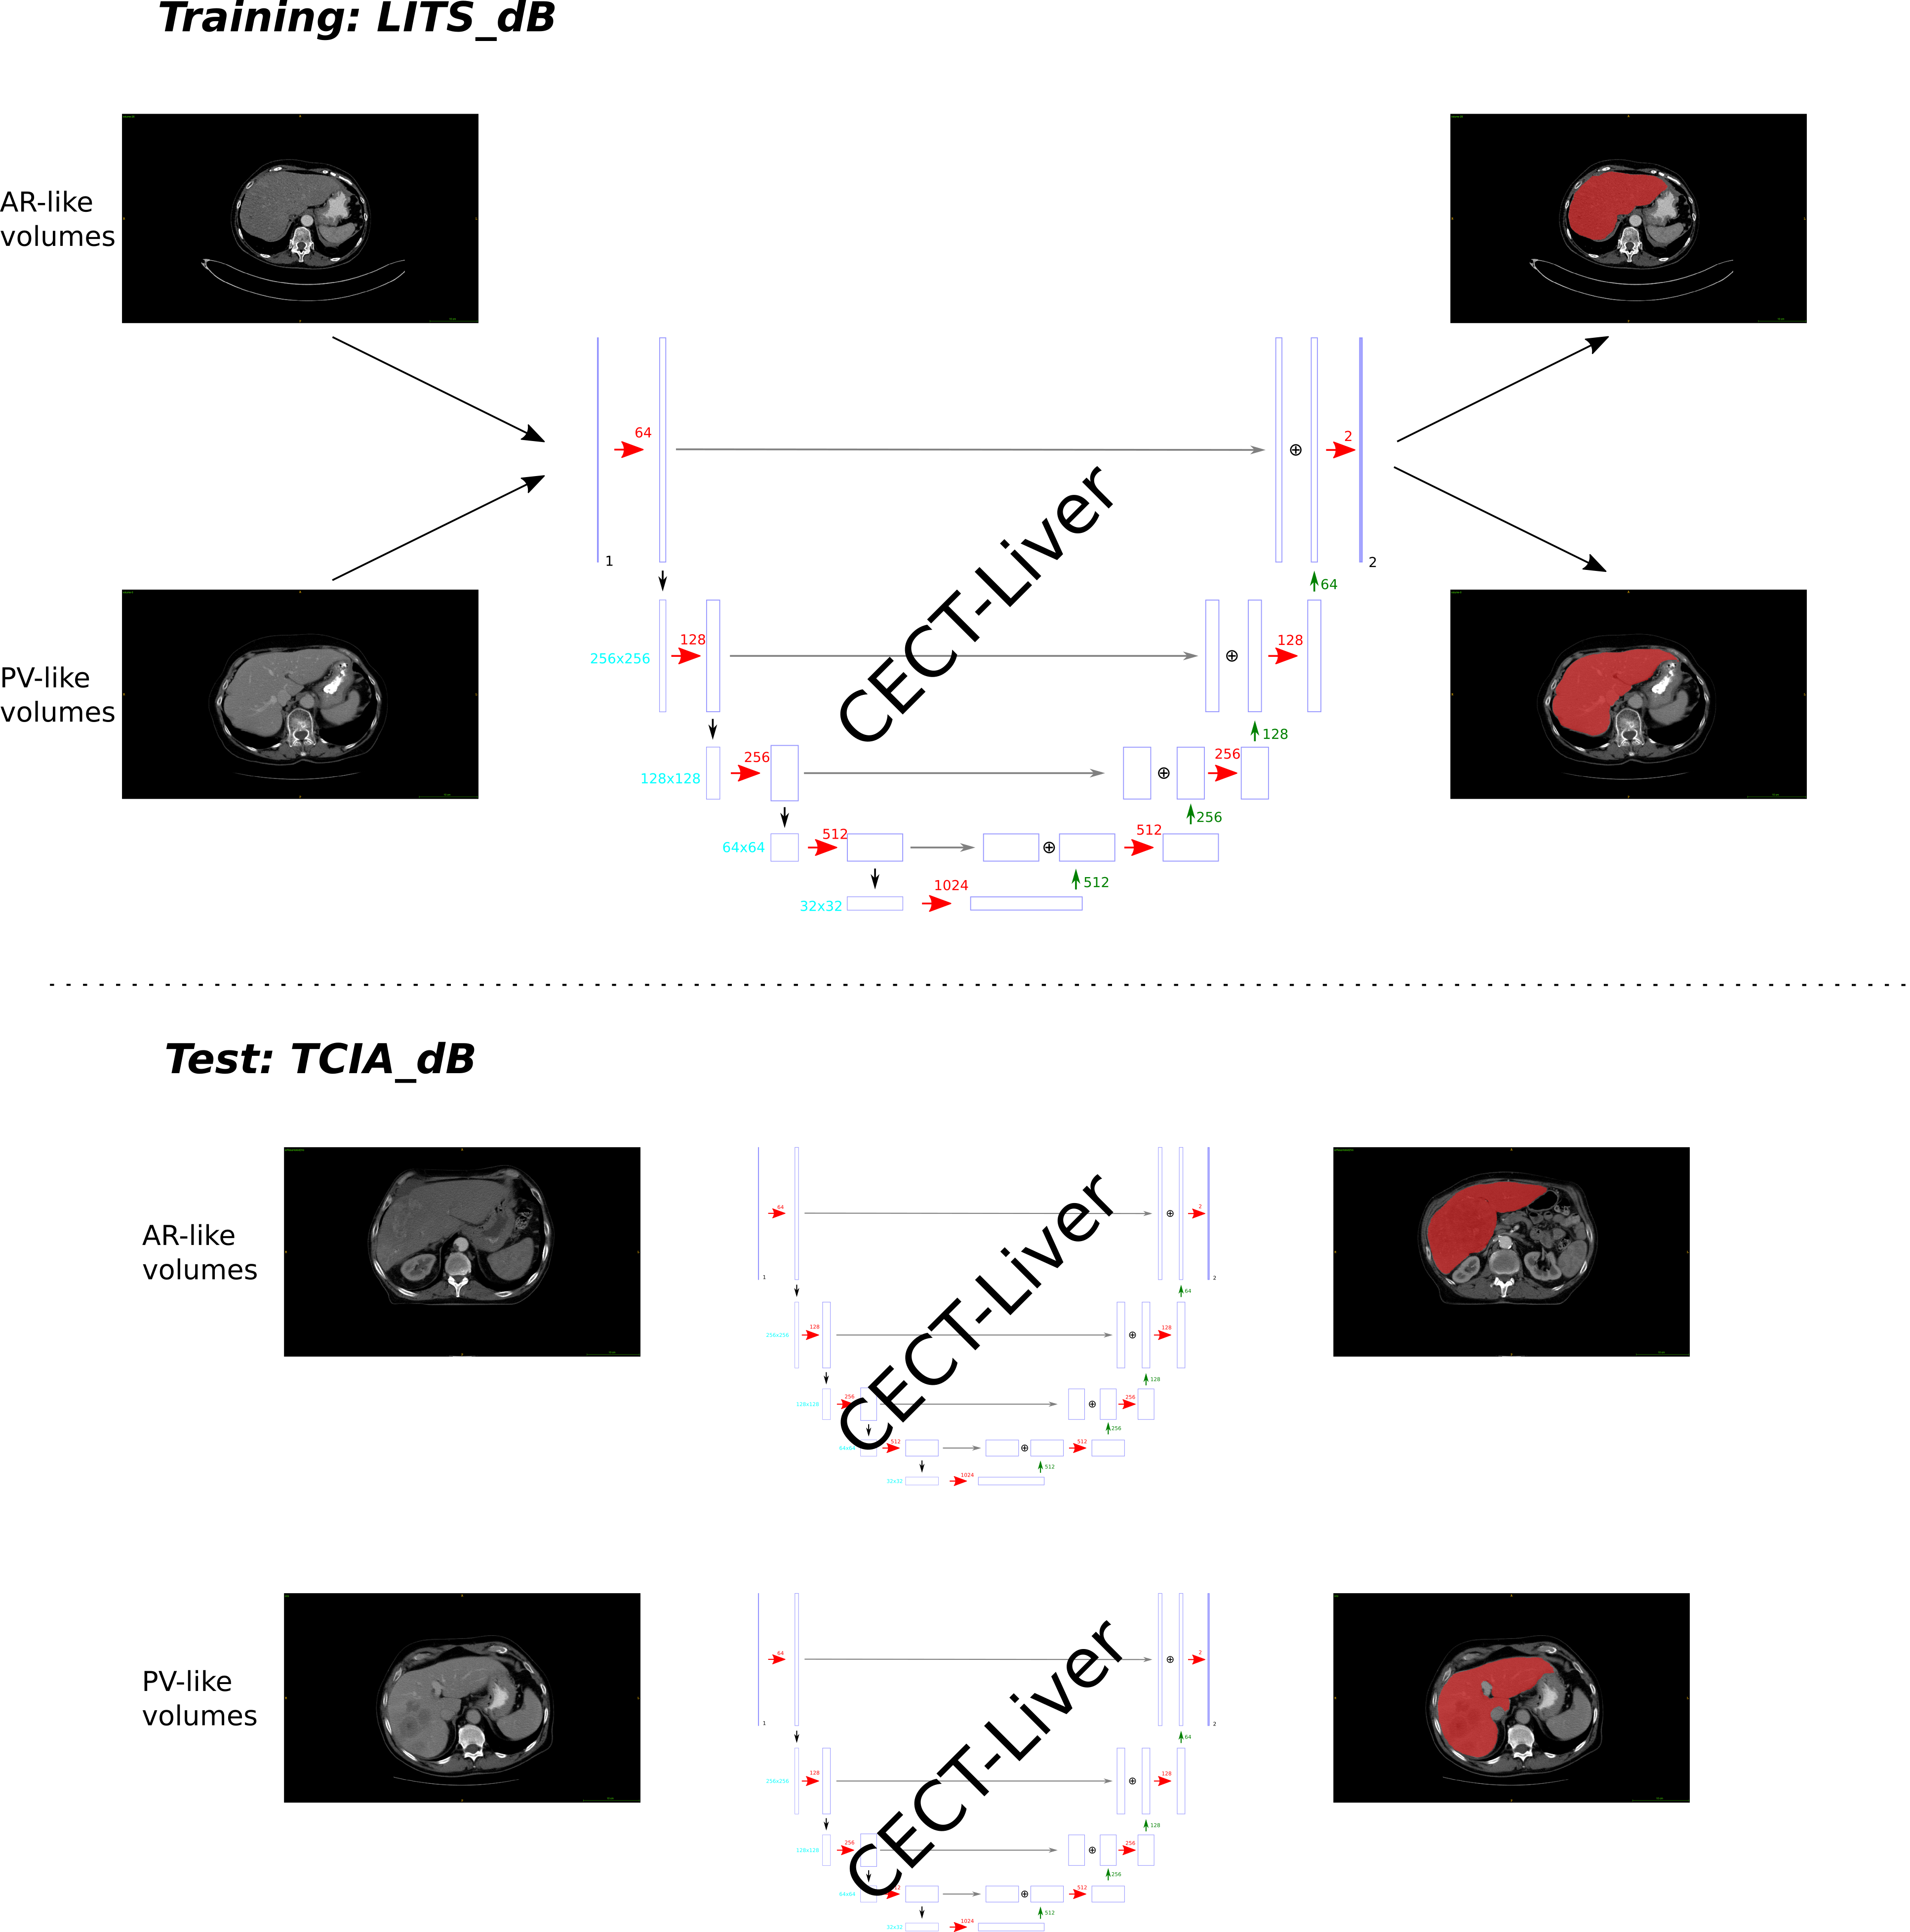
\includegraphics[width=\linewidth]{images/CECT_liver_details}
		\caption{We trained our network using each one of the 131 volumes of the \textbf{\lmttfont{LITS-dB}}, and tested the obtained architecture on both \ac{ar} and \ac{pv} \textbf{\lmttfont{TCIA-dB}} volumes. 
		}
		\label{fig:CECTliverDetails}
	\end{mdframed}
\end{figure}
}

\subsubsection{Results}\label{liver_segmentation_tcia_db_results}

When testing the \pplfont{\ac{cect}-Liver} network on \textbf{\lmttfont{TheraHCC-dB}} we
obtained a mean slice-wise \ac{dsc} of $ 90.4 \pm 17.5 $ on the \ac{pv} images and
$ 86.9 \pm 19.1 $ on the \ac{ar} images. These results, close to those obtained
in our previous work using a CV approach \cite{Ouhmich2019}, proved that \pplfont{\ac{cect}-Liver} can
perform liver segmentation on both \ac{ar} and \ac{pv} unseen images.
The \pplfont{CECT-Liver} network was also able to segment unseen volumes of the
\textbf{\lmttfont{TCIA-dB}} in both \ac{ar} and \ac{pv} phases even when the liver presents a big
lesion, as we can see in the figure \ref{fig:LiverPredTciaDb}.
Even though the overall visual predictions seemed very accurate, some mis-segmentation cases have been noticed. Liver segmentation errors often appear on top/bottom axial slices and are often due to our 2D approach, where the 3D context is lost, and where it is often very difficult to see the extremity of the liver in a single slice, as depicted in the figure \ref{fig:LITS_networkMisSeg_extremSlices}. As exposed previously the main drawback of our approach corresponds to cases where the missed liver segment is occupied by a liver tumor (see \ref{fig:LITS_networkMisSeg_extremSlices} and \ref{fig:LITS_networkMisSeg_tumor}).
As explained earlier, an other problem often occurring is the mis-segmentation of other abdominal organs, that are sometimes considered as being part of the liver. However, our post-processing steps usually correct these mistakes by removing the undesired tissues from the final segmentation map (as illustrated in the figure \ref{fig:LITS_networkMisSeg_otherOrgans}).


\begin{figure}[ht!]
\centering
\begin{minipage}{0.45\linewidth}
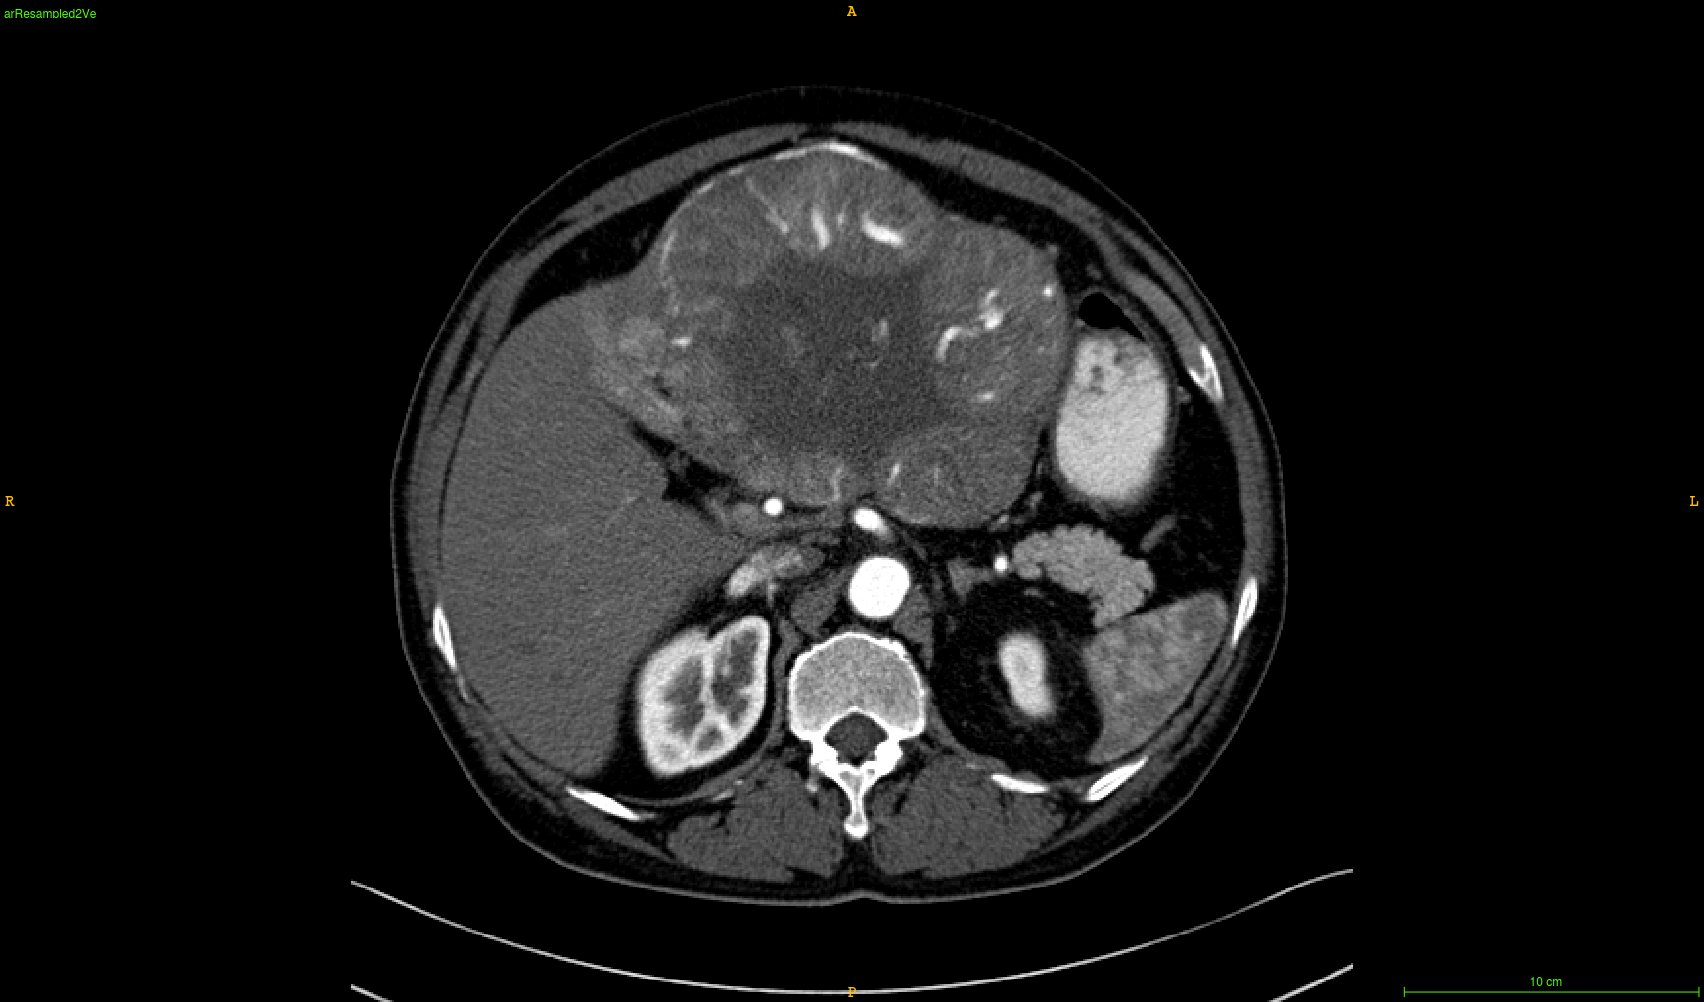
\includegraphics[width=0.9\linewidth]{../HistologicalGradePrediction/images/TCIA_CECTLiver_prediction_TCGA-DD-A11A_slice42_AR_raw}
\end{minipage}
\hspace{0.3cm}
\begin{minipage}{0.45\linewidth}
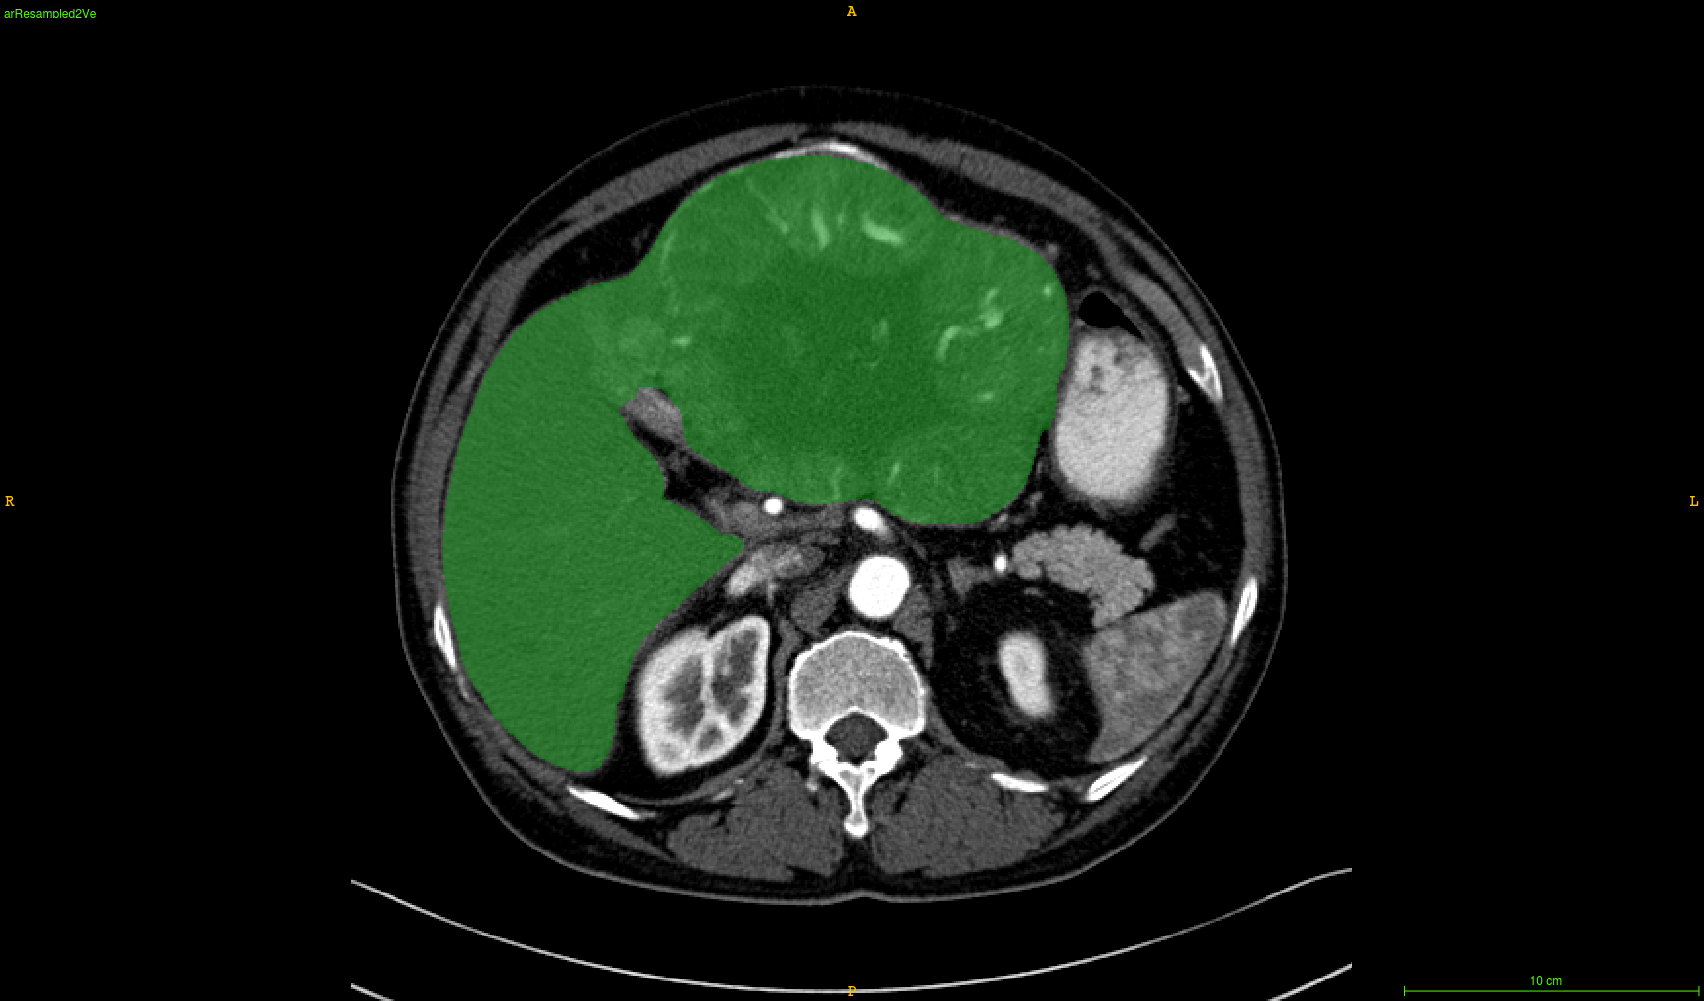
\includegraphics[width=0.9\linewidth]{../HistologicalGradePrediction/images/TCIA_CECTLiver_prediction_TCGA-DD-A11A_slice42_AR_green_liver}
\end{minipage}

\vspace{0.8cm}
\begin{minipage}{0.45\linewidth}
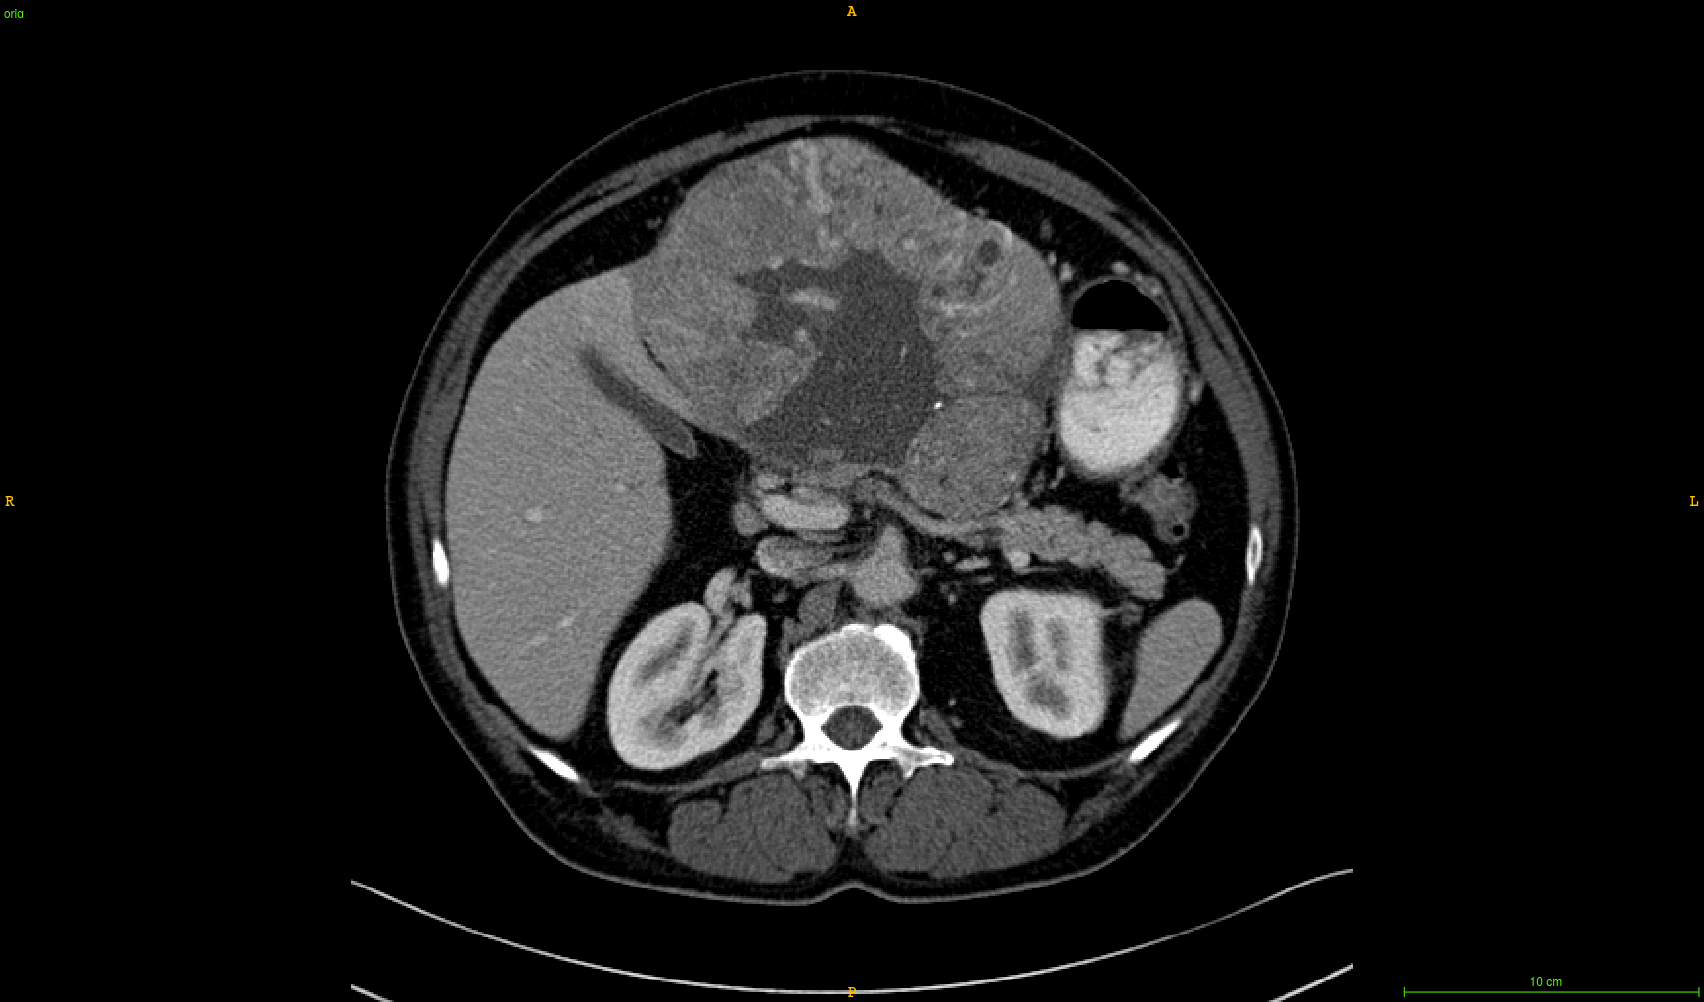
\includegraphics[width=0.9\linewidth]{../HistologicalGradePrediction/images/TCIA_CECTLiver_prediction_TCGA-DD-A11A_slice42_raw}
\end{minipage}
\hspace{0.3cm}
\begin{minipage}{0.45\linewidth}
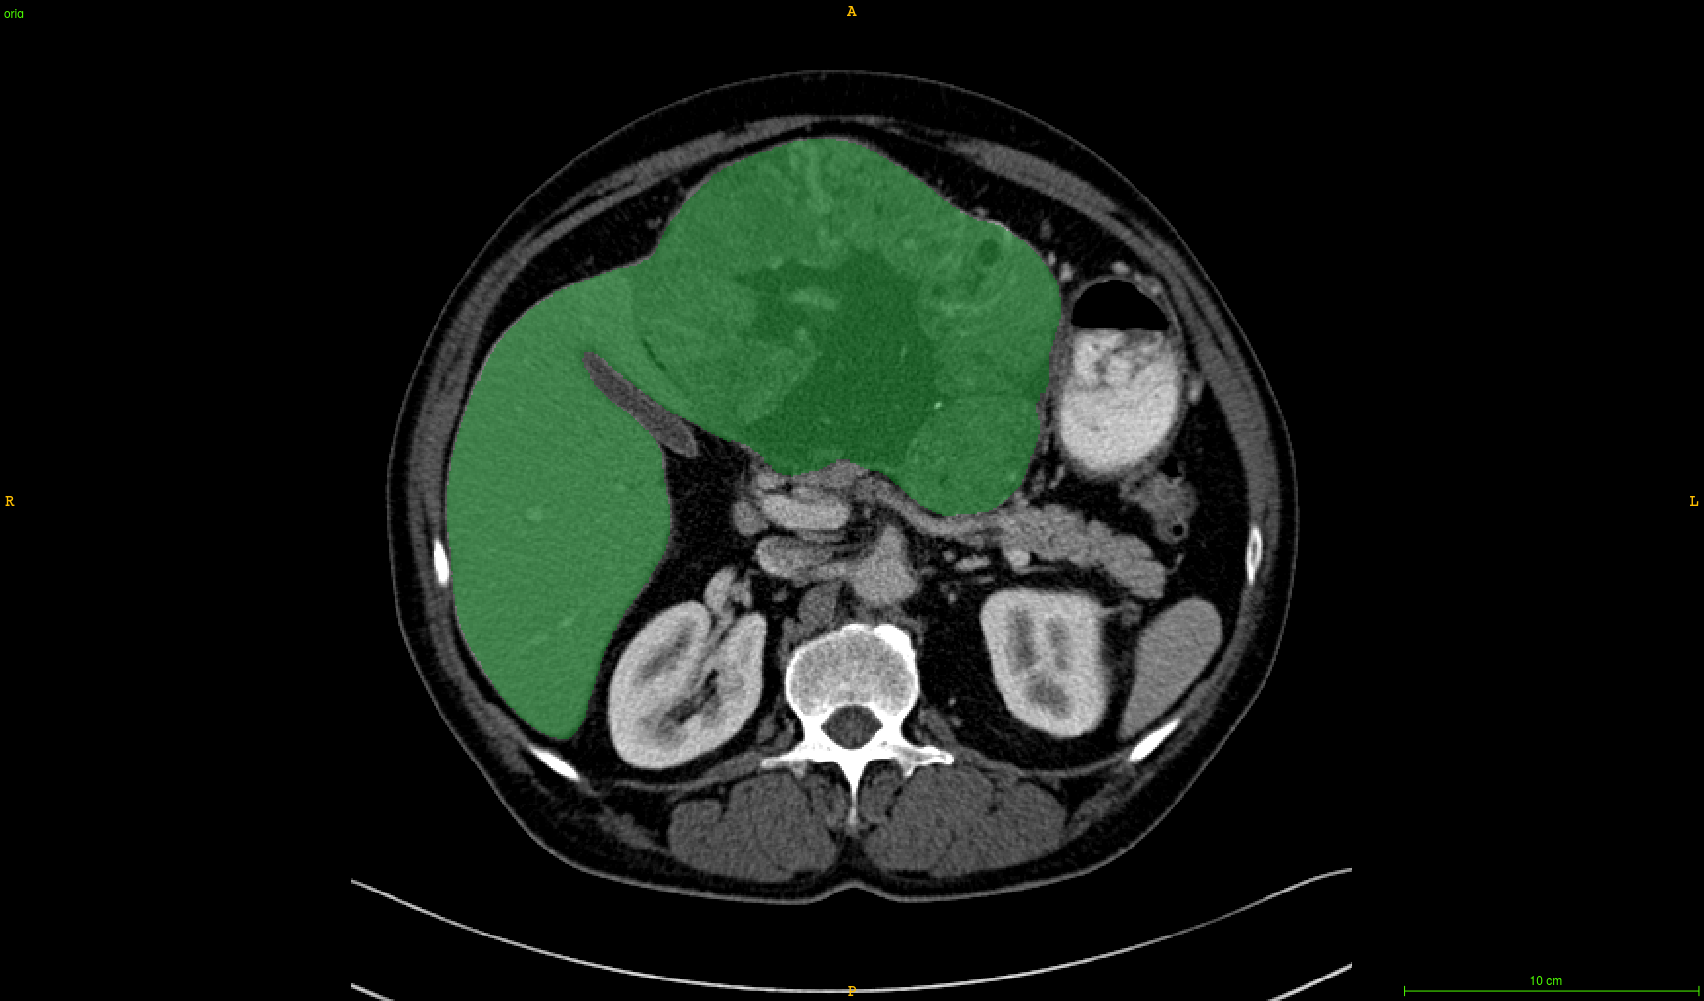
\includegraphics[width=0.9\linewidth]{../HistologicalGradePrediction/images/TCIA_CECTLiver_prediction_TCGA-DD-A11A_slice42_greenLiver}
\end{minipage}
\caption{Example of liver segmentation using the \pplfont{\ac{cect}-Liver} network on \textbf{\lmttfont{TCIA-dB}}
patients (Top row \ac{ar} images, bottom row: \ac{pv} images, left:
Raw images, right : liver segmentation as overlay).}
\label{fig:LiverPredTciaDb}
\end{figure}

\begin{figure}[ht!]
	\begin{mdframed}[backgroundcolor=blue!50,linecolor=blue!50]
		\centering
		\begin{minipage}{0.45\linewidth}
			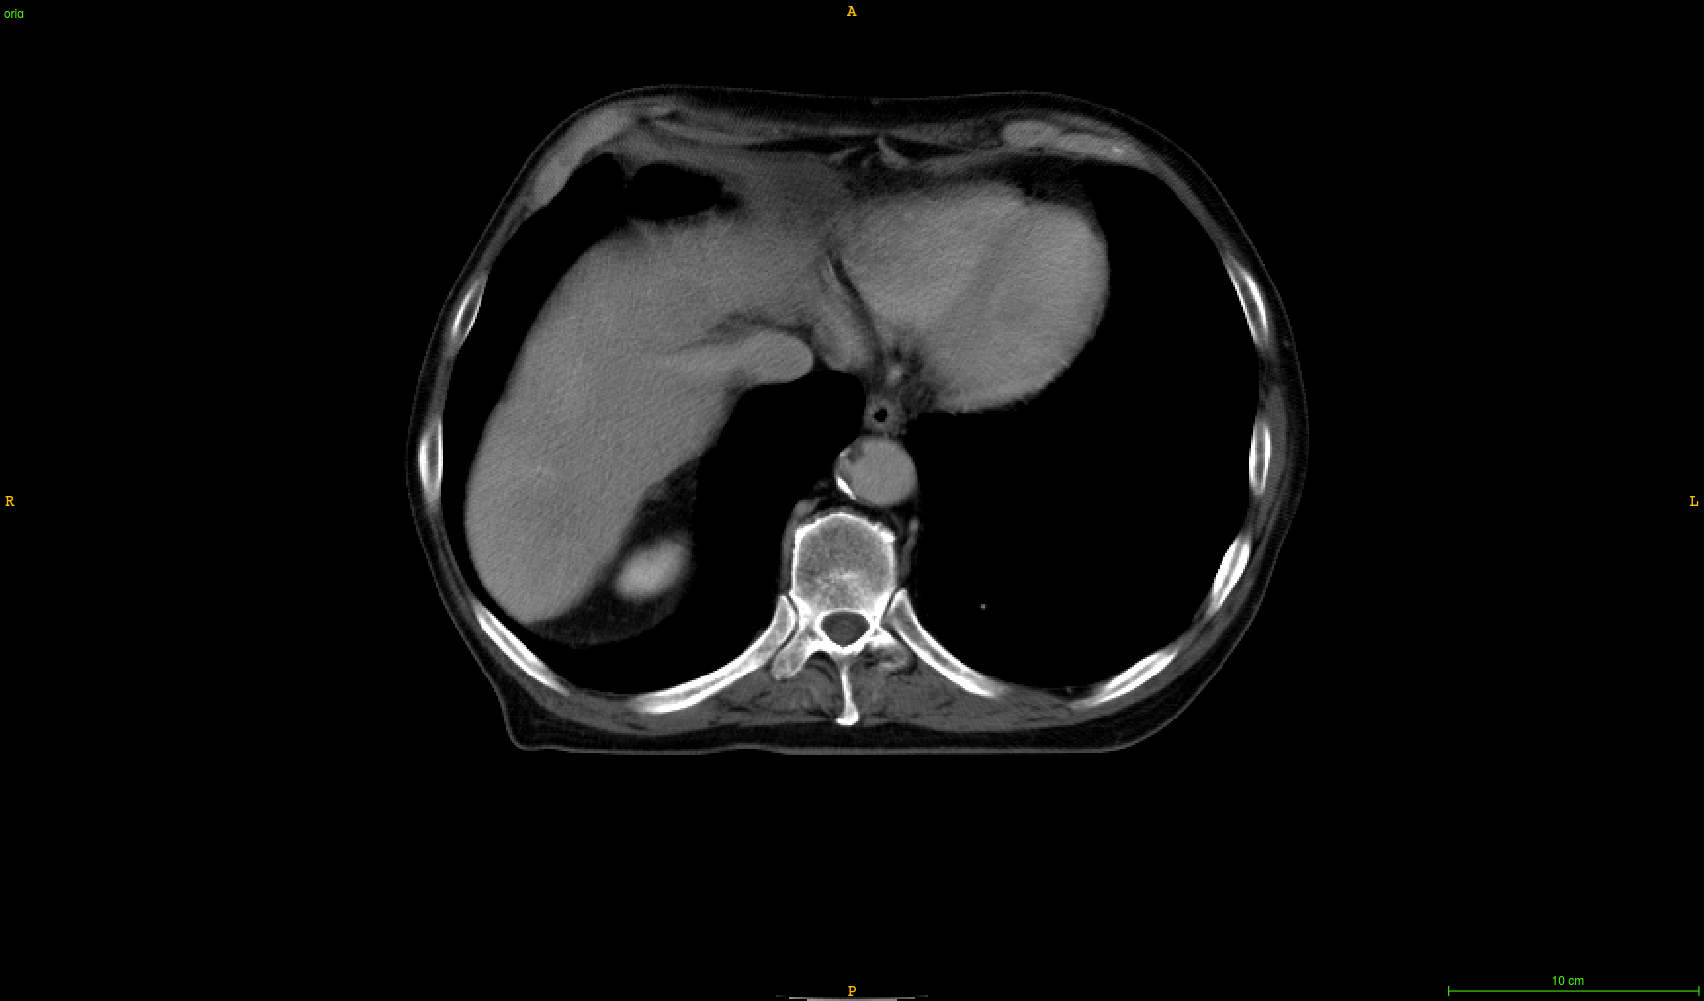
\includegraphics[width=\linewidth]{images/MisSegmentations/TCGA-DD-A3A1_slice80_raw}
		\end{minipage} \hspace{-0.1cm}
		\begin{minipage}{0.45\linewidth}
			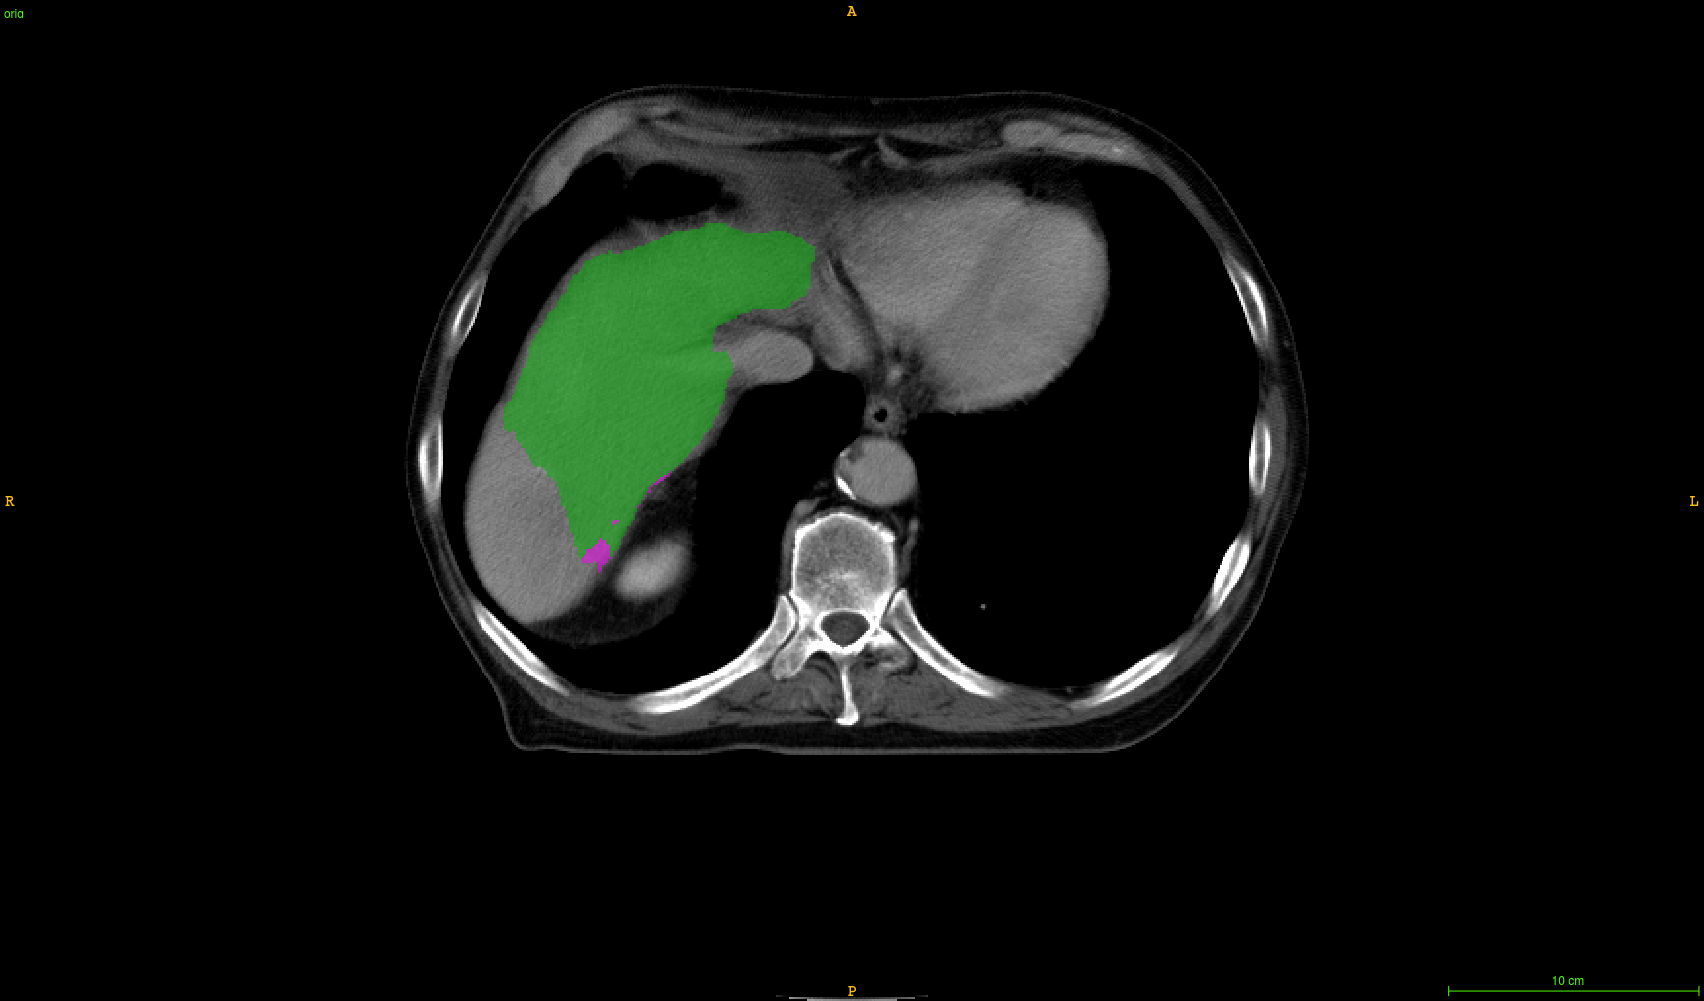
\includegraphics[width=\linewidth]{images/MisSegmentations/TCGA-DD-A3A1_slice80_liverPrediction_Cmap}
		\end{minipage} \\
		\begin{minipage}{0.45\linewidth}
			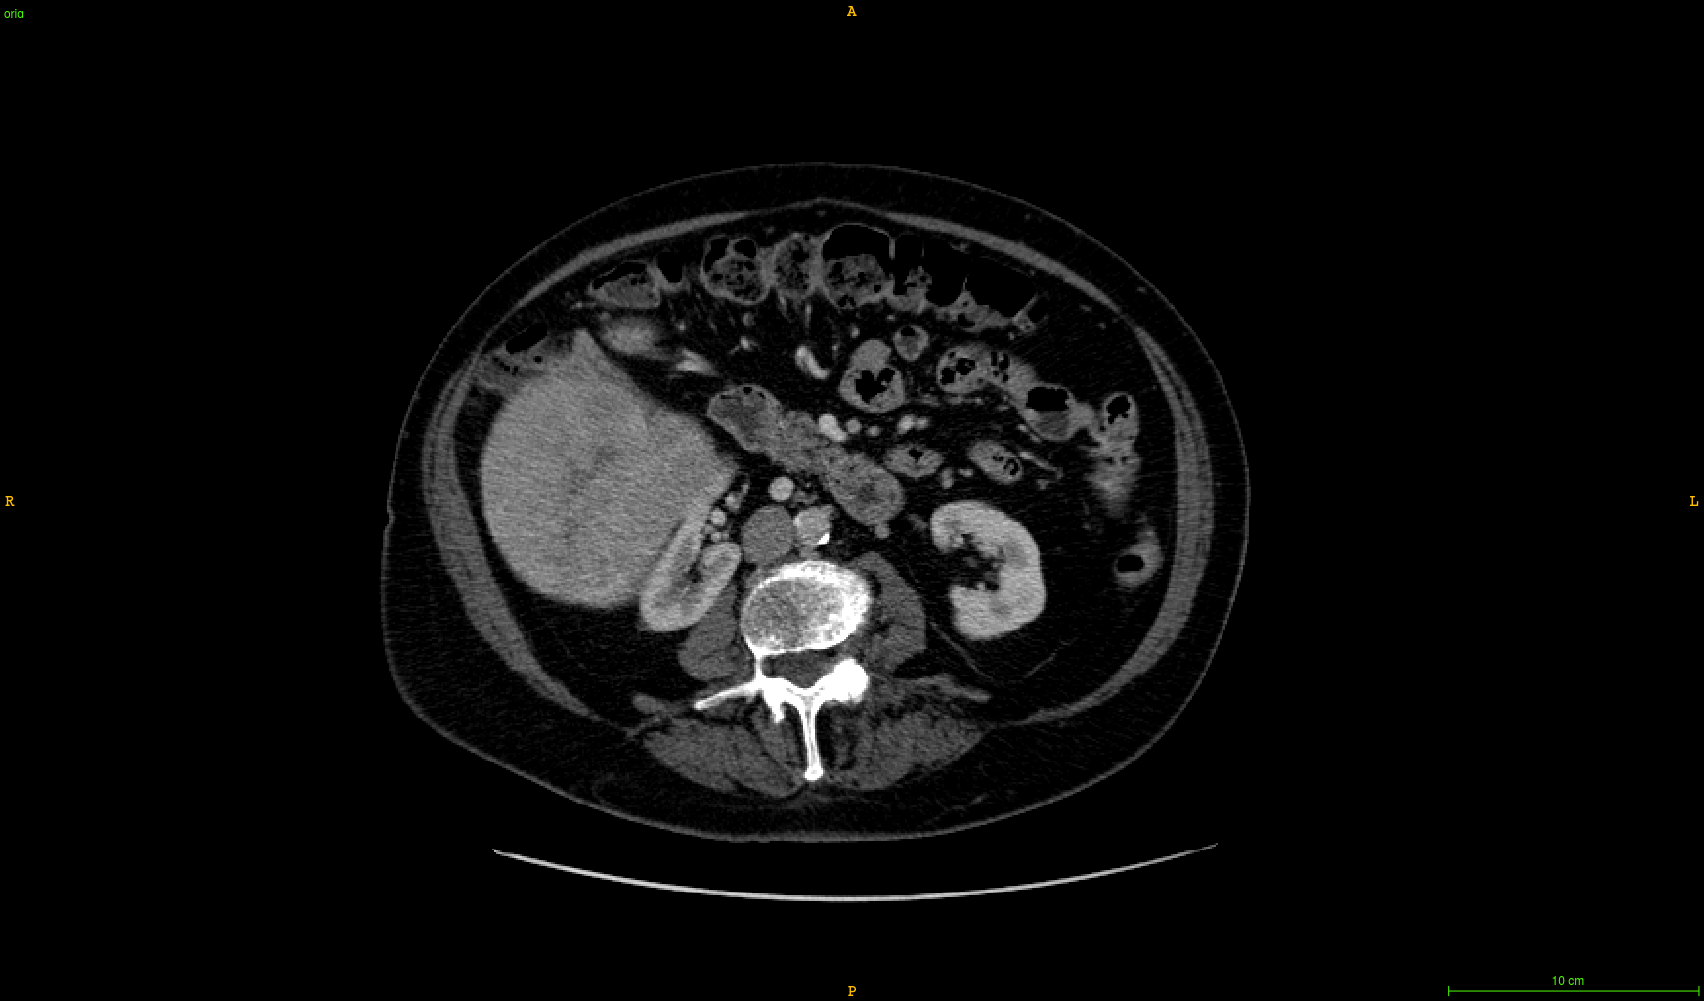
\includegraphics[width=\linewidth]{images/MisSegmentations/TCGA-DD-A4NK_slice32_raw}
		\end{minipage} \hspace{-0.1cm}
		\begin{minipage}{0.45\linewidth}
			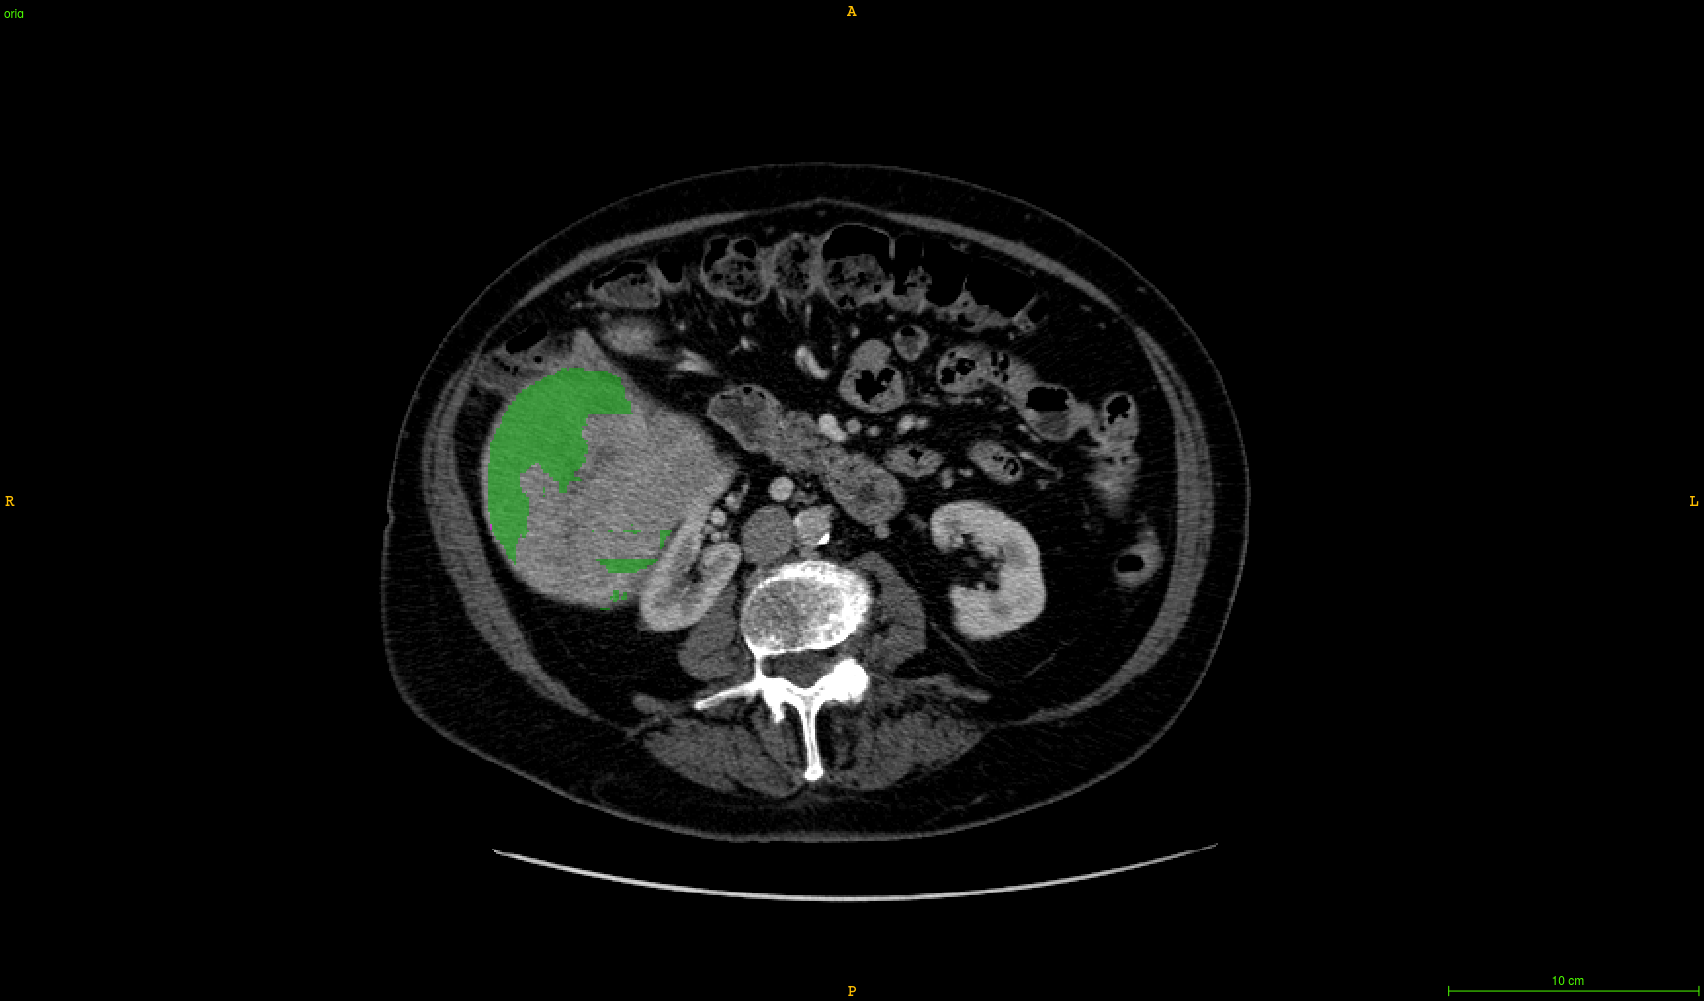
\includegraphics[width=\linewidth]{images/MisSegmentations/TCGA-DD-A4NK_slice32_liverPrediction_Cmap}
		\end{minipage} \\
		\begin{minipage}{0.45\linewidth}
			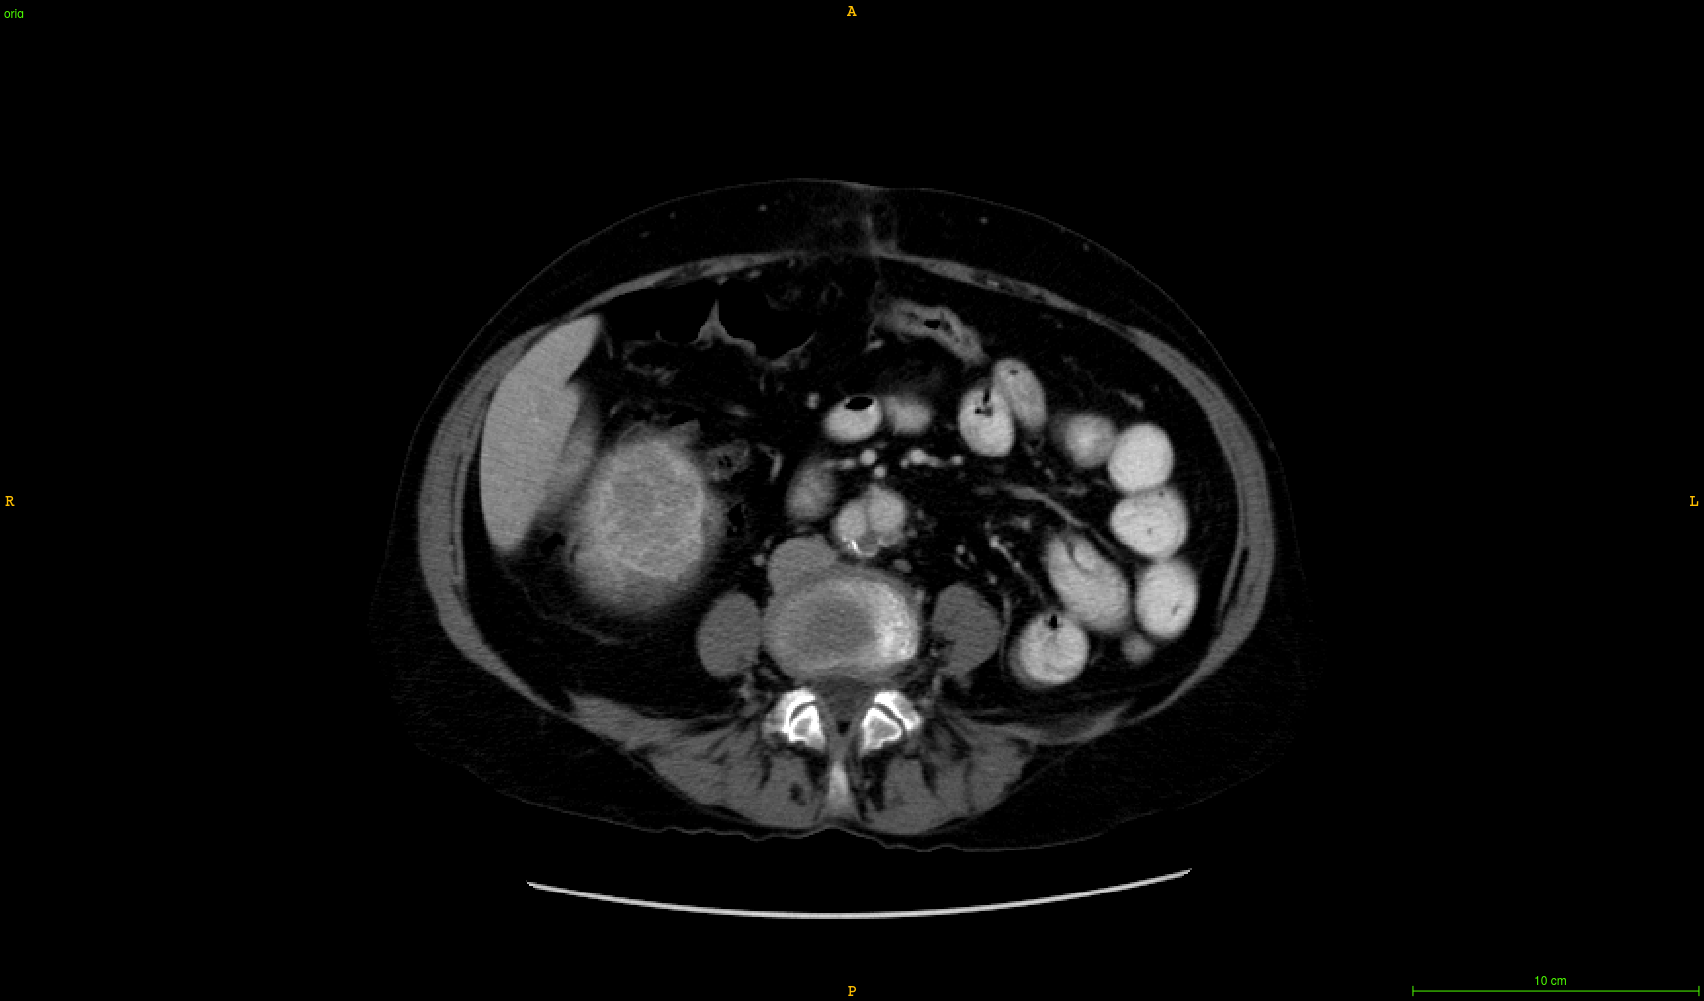
\includegraphics[width=\linewidth]{images/MisSegmentations/TCGA-DD-A1EB_slice9_raw}
		\end{minipage} \hspace{-0.1cm}
		\begin{minipage}{0.45\linewidth}
			\includegraphics[width=\linewidth]{images/MisSegmentations/TCGA-DD-A1EB_slice9_liverPrediction_Cmap_Arrow}
		\end{minipage}
		\caption{Examples of liver mis-segmentation cases with left being the raw images and right being the liver segmentation prediction obtained by our \pplfont{\ac{cect}-Liver} network (green area corresponds to the retained liver segmentation, whereas the purple area corresponds to voxels removed by the post-processing steps). Top row depicts an axial top liver slice, where nearly half of the liver has been missed. Second row depicts a bottom liver slice where a big portion of the liver occupied by a tumor has been missed by the liver segmentation. Bottom row also depicts a bottom liver slices where a small portion is missed by the network, but the hepatic lesion is missed as well (green arrow).}
		\label{fig:LITS_networkMisSeg_extremSlices}
	\end{mdframed}
\end{figure}

\begin{figure}[ht!]
	\begin{mdframed}[backgroundcolor=blue!50,linecolor=blue!50]
		\centering
		\begin{minipage}{0.45\linewidth}
			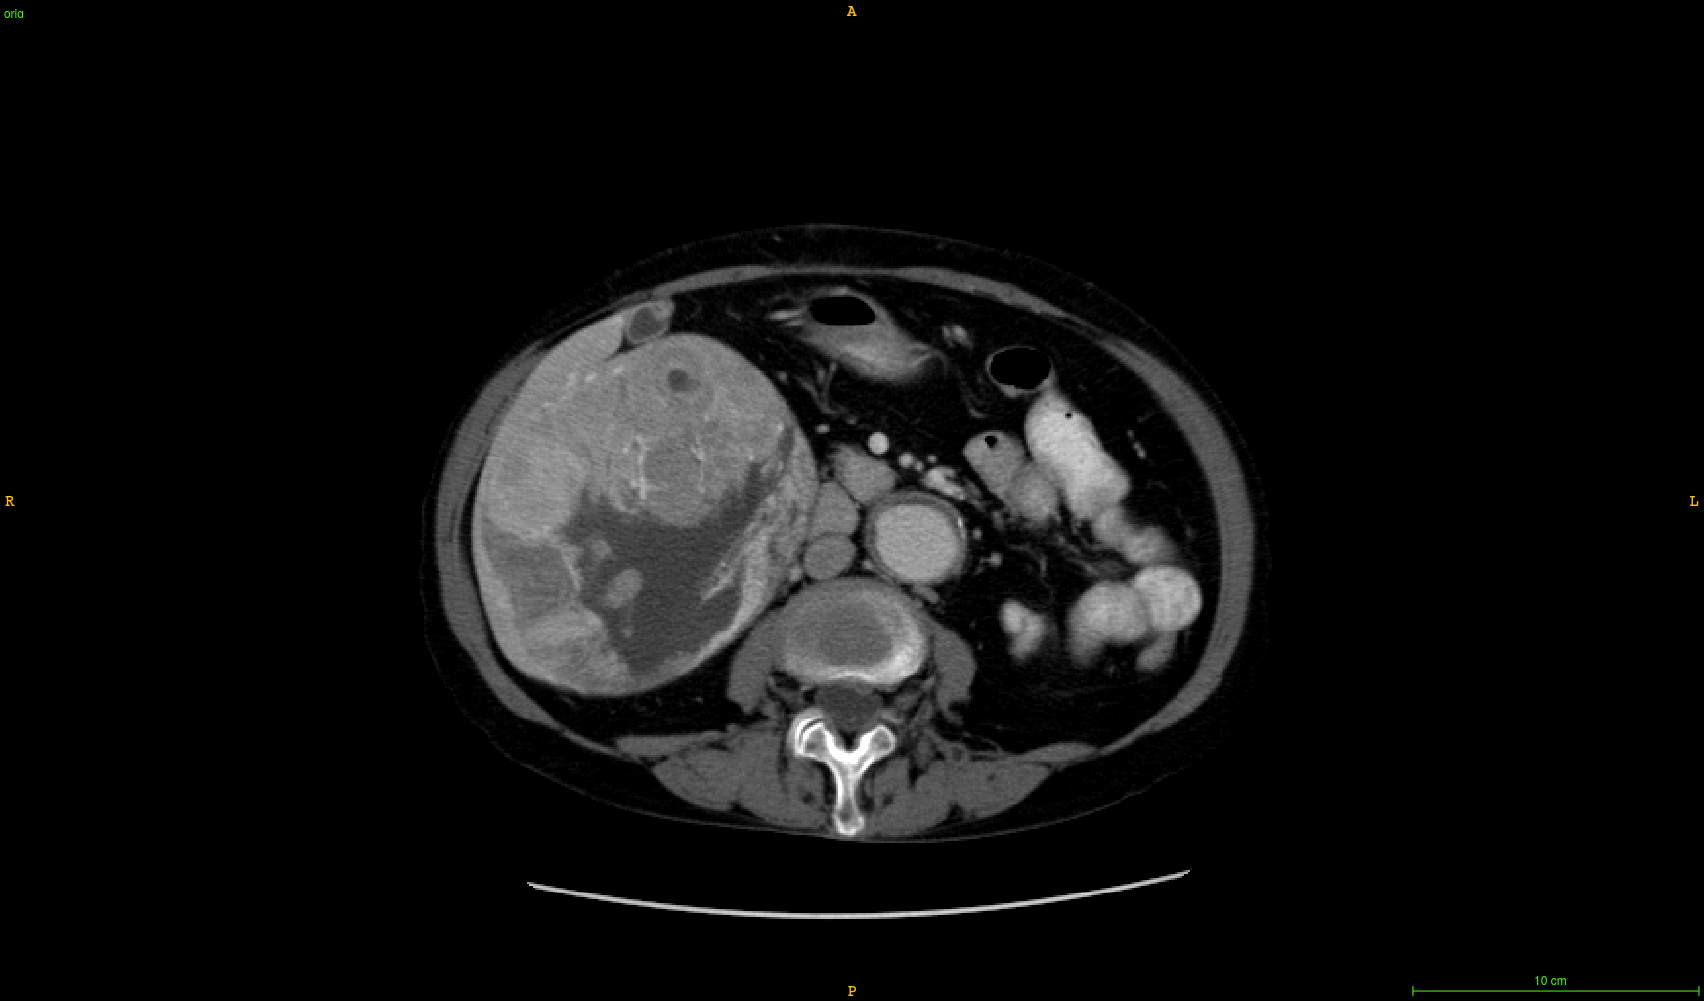
\includegraphics[width=\linewidth]{images/MisSegmentations/TCGA-DD-A1EB_slice16_raw}
		\end{minipage} \hspace{-0.1cm}
		\begin{minipage}{0.45\linewidth}
			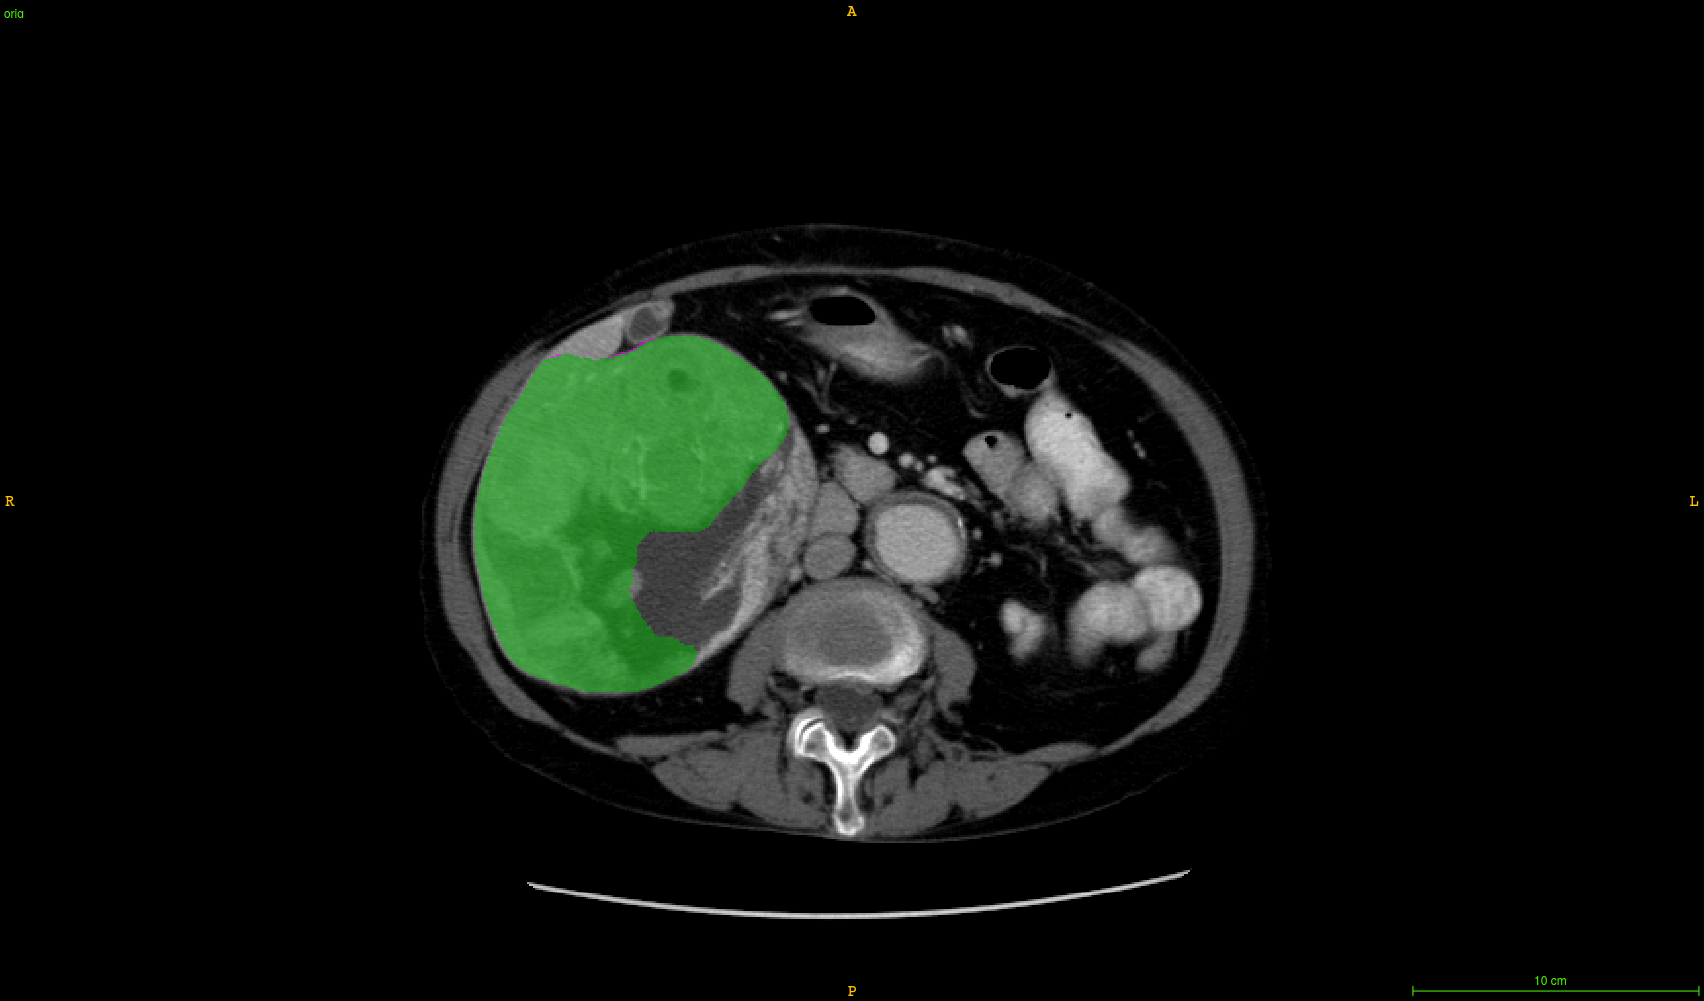
\includegraphics[width=\linewidth]{images/MisSegmentations/TCGA-DD-A1EB_slice16_liverPrediction_Cmap}
		\end{minipage}
		\caption{Example of liver mis-segmentation where a big portion of the lesion has been missed by our liver segmentation network. In this specific case, the portion of the tumor that has been missed corresponded to the necrotic area which was remarkably darker than usual (less than 10HU).}
		\label{fig:LITS_networkMisSeg_tumor}
	\end{mdframed}
\end{figure}

\begin{figure}[ht!]
	\begin{mdframed}[backgroundcolor=blue!50,linecolor=blue!50]
		\centering
		\begin{minipage}{0.45\linewidth}
			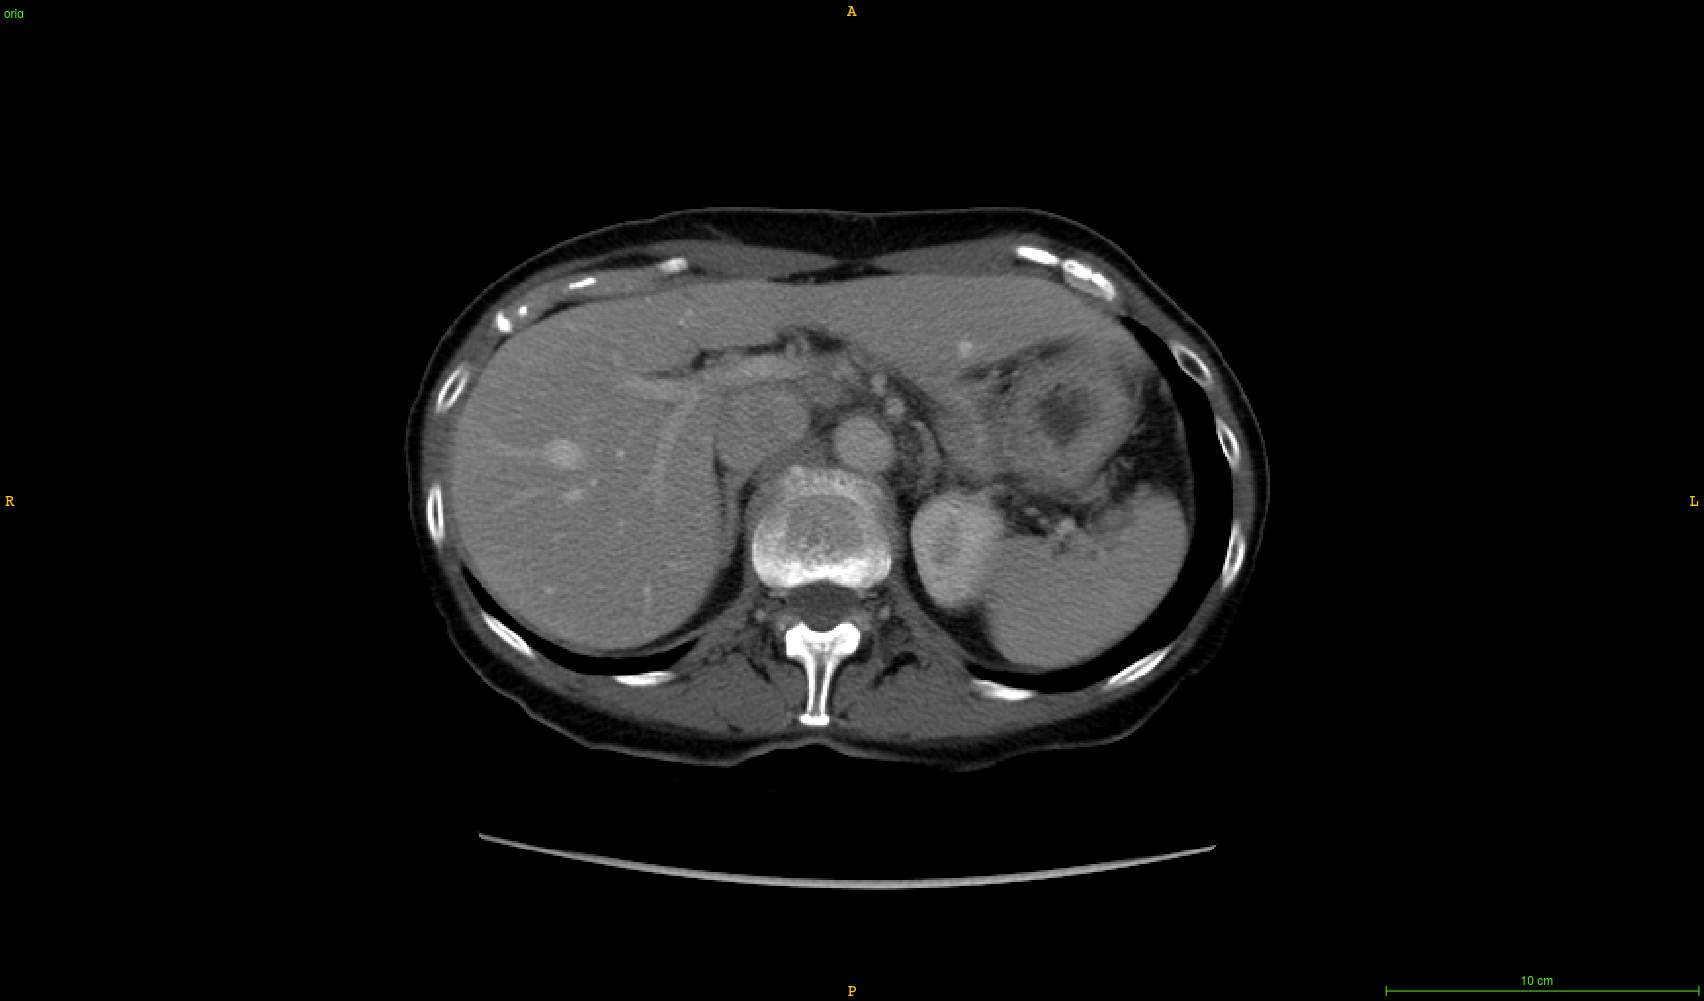
\includegraphics[width=\linewidth]{images/MisSegmentations/TCGA-BC-A3KF_slice61_raw}
		\end{minipage} \hspace{-0.1cm}
		\begin{minipage}{0.45\linewidth}
			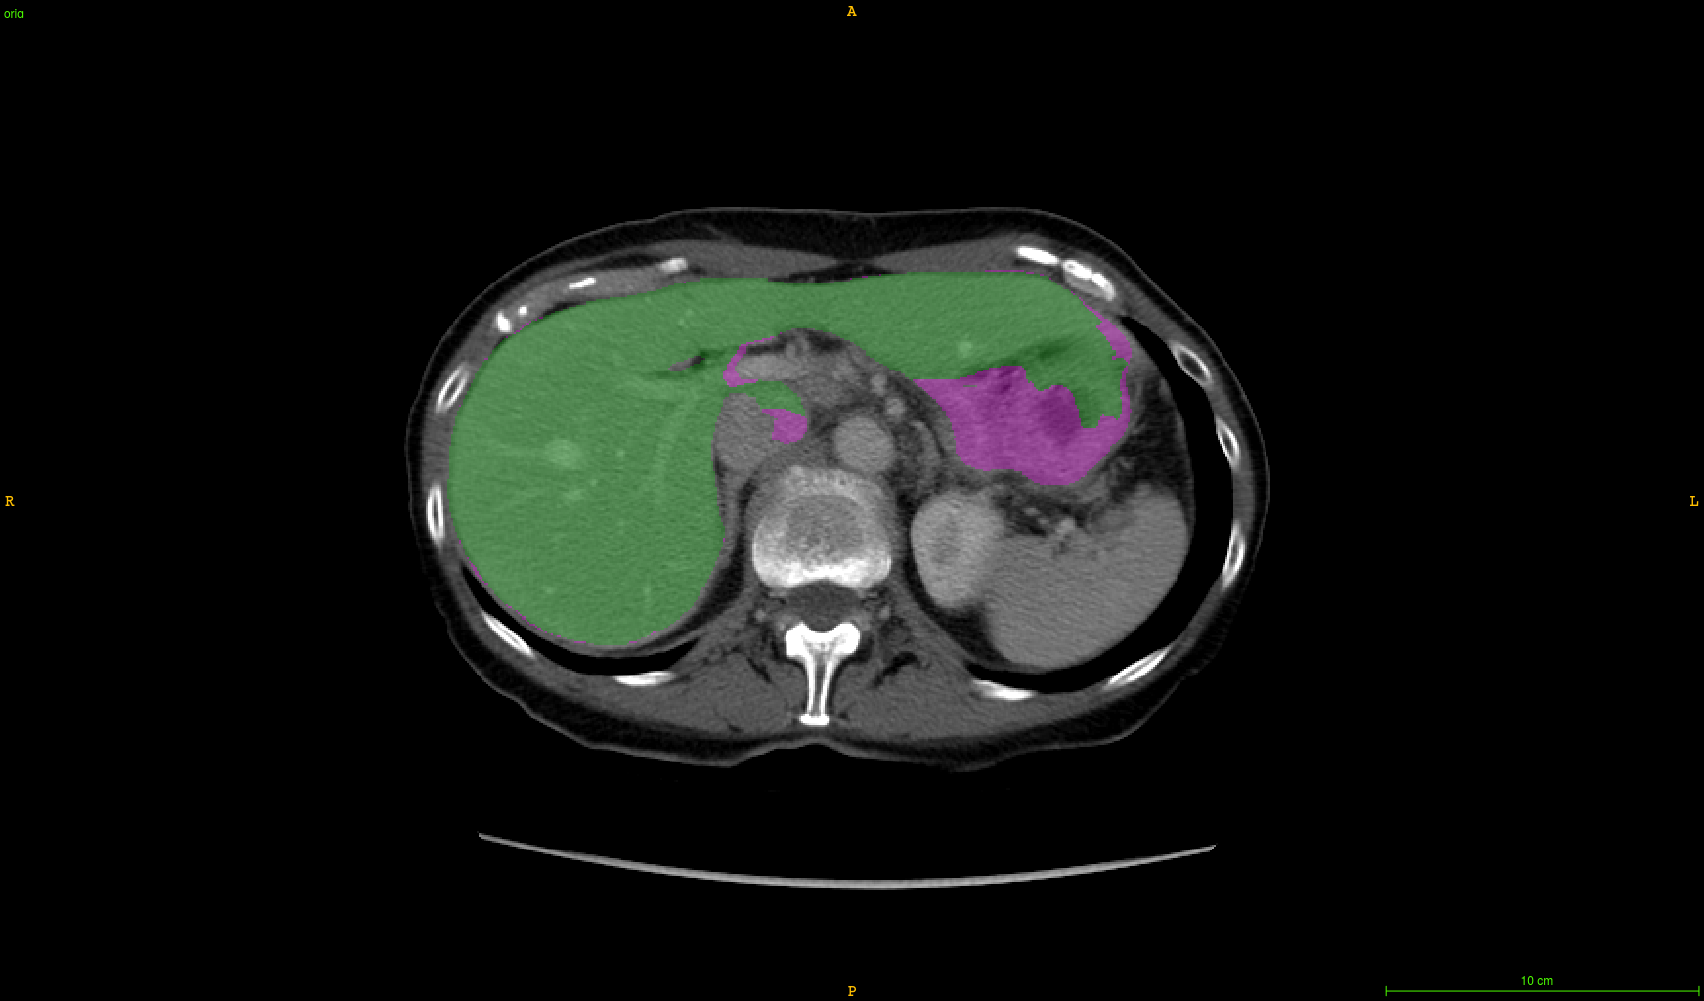
\includegraphics[width=\linewidth]{images/MisSegmentations/TCGA-BC-A3KF_slice61_liverPrediction_Cmap}
		\end{minipage} \\
		\begin{minipage}{0.45\linewidth}
			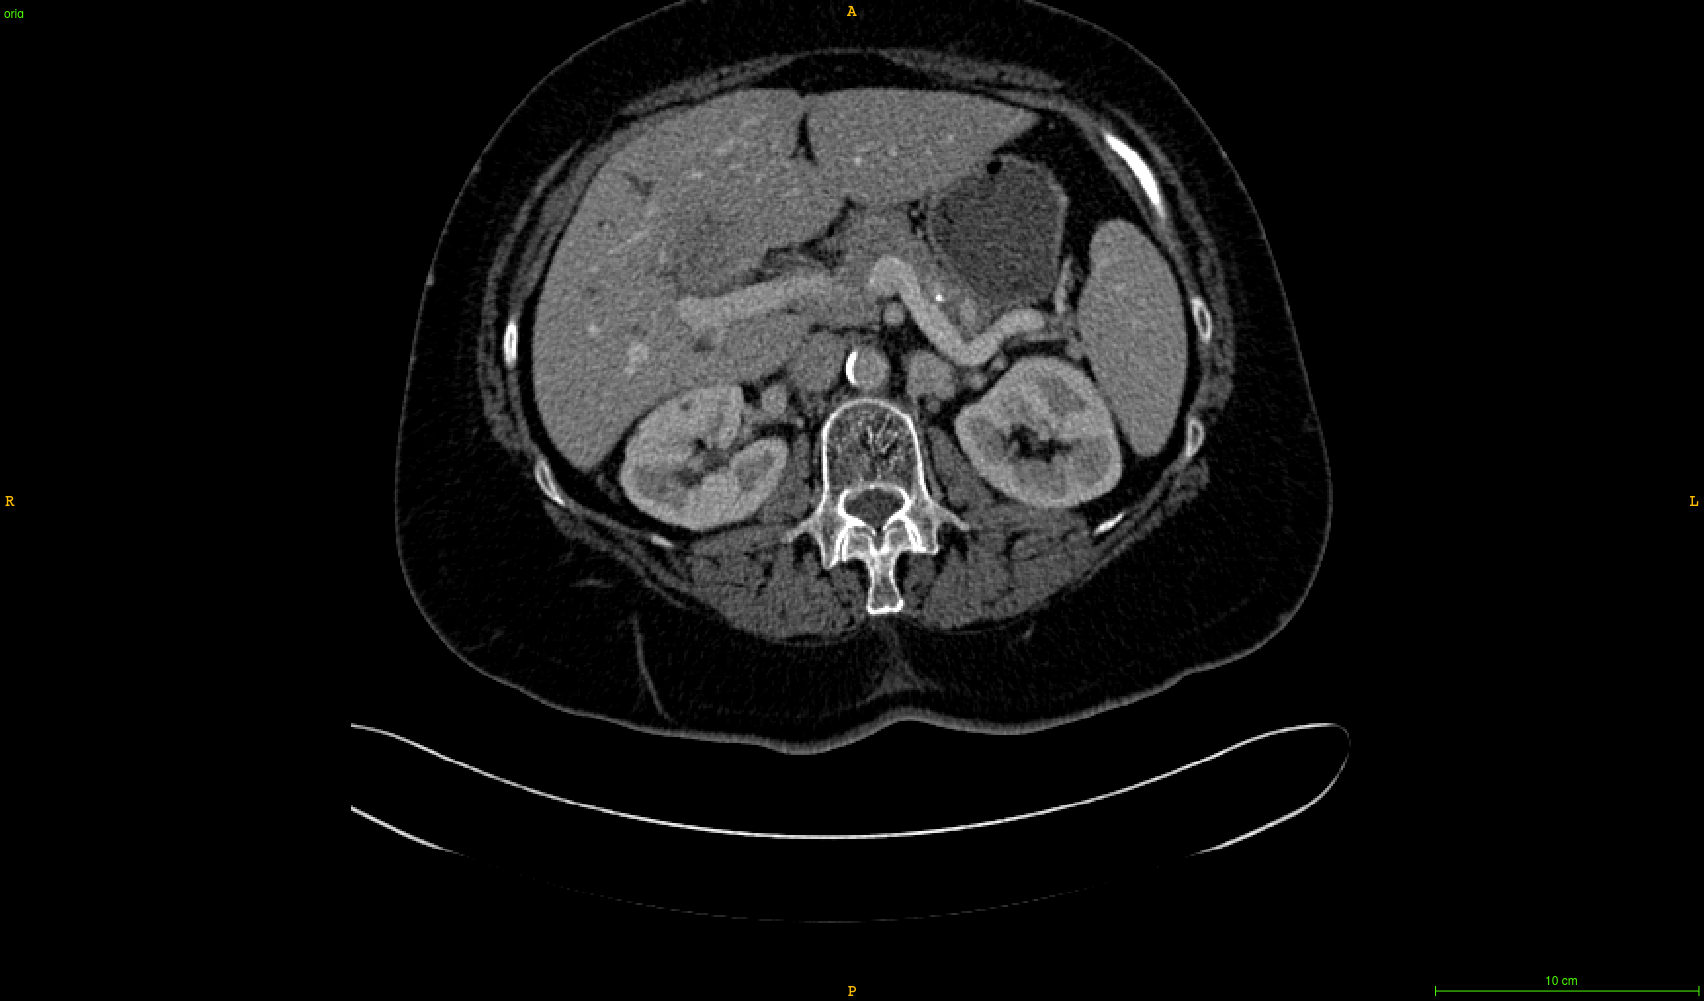
\includegraphics[width=\linewidth]{images/MisSegmentations/TCGA-BC-A10Z_slice30_raw}
		\end{minipage} \hspace{-0.1cm}
		\begin{minipage}{0.45\linewidth}
			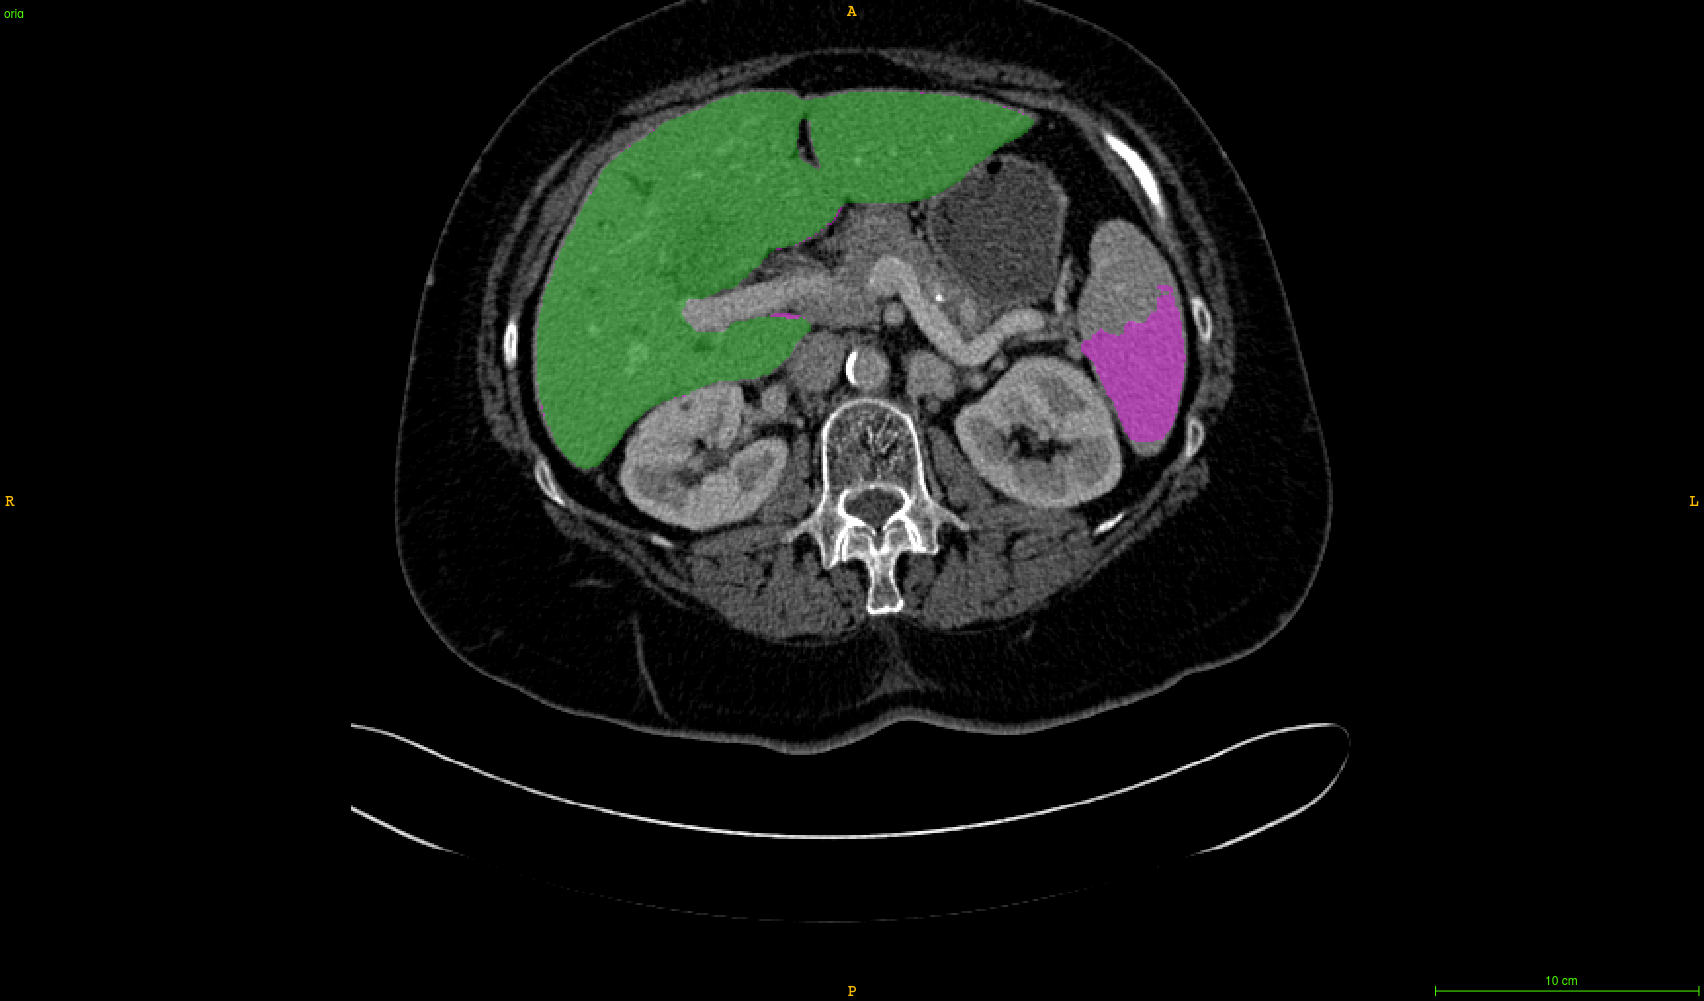
\includegraphics[width=\linewidth]{images/MisSegmentations/TCGA-BC-A10Z_slice30_liverPrediction_Cmap}
		\end{minipage} \\
		\begin{minipage}{0.45\linewidth}
			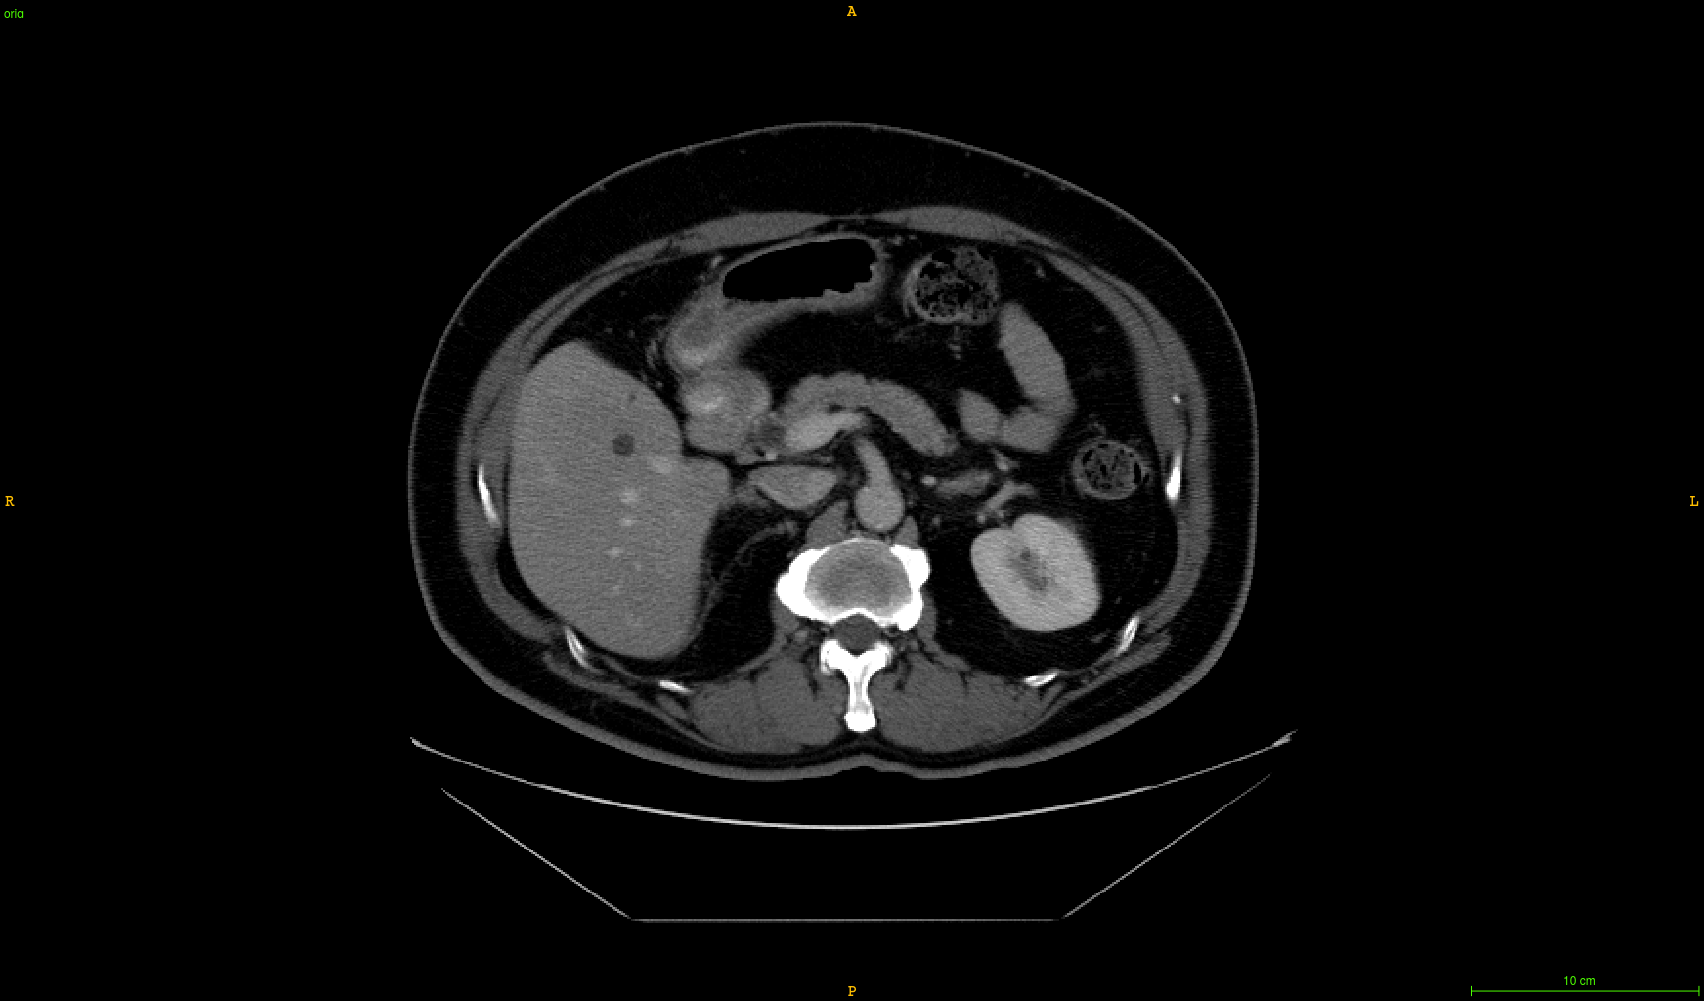
\includegraphics[width=\linewidth]{images/MisSegmentations/TCGA-DD-A1EA_slice30_raw}
		\end{minipage} \hspace{-0.1cm}
		\begin{minipage}{0.45\linewidth}
			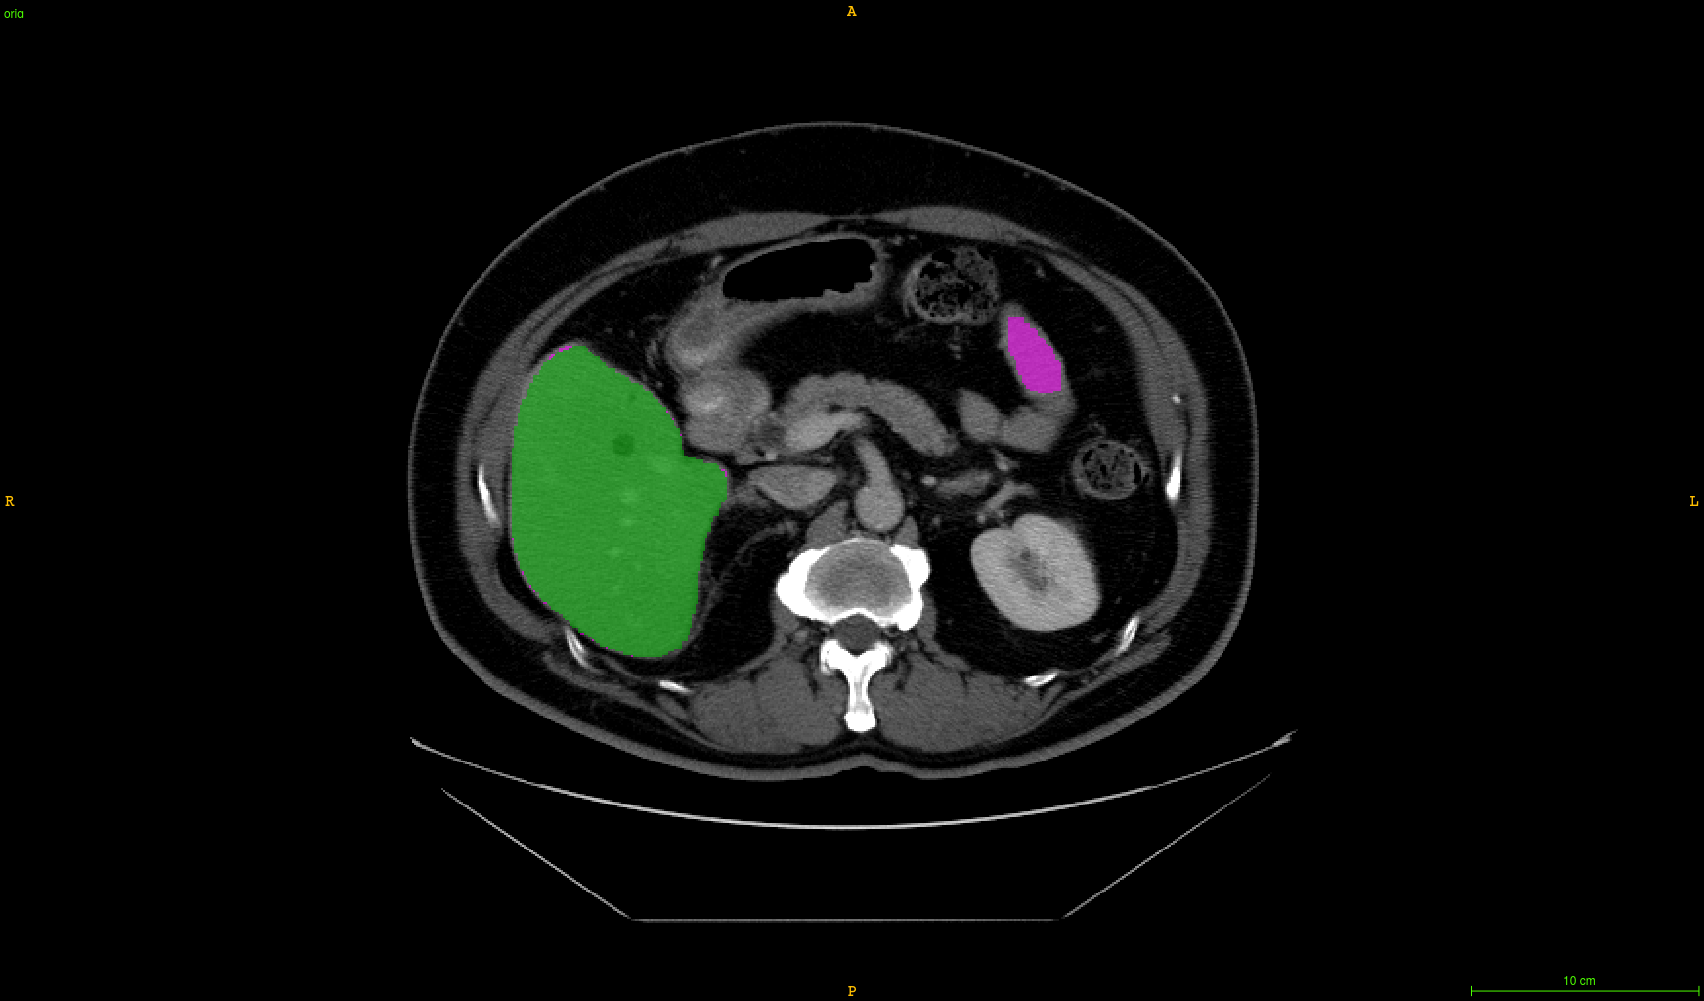
\includegraphics[width=\linewidth]{images/MisSegmentations/TCGA-DD-A1EA_slice30_liverPrediction_Cmap}
		\end{minipage}
		\caption{Examples of liver mis-segmentation cases with left being the raw images and right being the liver segmentation prediction obtained by our \pplfont{\ac{cect}-Liver} network (green area corresponds to the retained liver segmentation, whereas the purple area corresponds to voxels removed by the post-processing steps). In the given examples we have the stomach (top row), the spleen (second row) and the colon (bottom row) that have been mis-interpreted by the network as being part of the liver, however in each case the post-processing steps allowed us to remove the unwanted tissue from the remaining segmentation map.}
		\label{fig:LITS_networkMisSeg_otherOrgans}
	\end{mdframed}
\end{figure}

Once a robust liver segmentation was obtained, we implemented our
registration pipeline.

We have decided to implement the registration pipeline using ANTs \cite{avants2009advanced}, since it has already been used for liver
CT scans registration \cite{Zhao2019,Zhao2020}.

\subsection{ANTs registration}\label{tcia-db-ants-registration}

The classical ANTs registration pipeline is made of 3 steps. The first
two steps consist of linear transformations, where a rigid
transformation is first applied, followed by an affine transformation.
The last one is generally non-linear. In our pipeline,
we used a Syn (\emph{Standard Symmetric normalisation}) transformation, which
processes a gradient field, determining how each point of the space will
shift \cite{Avants2008}.

The MI (Mutual Information) was used as loss function for the first two
steps because it has the advantage of computing the similarity at a
large scale. Linear rigid and affine transformations tend to roughly bring both volumes
in the same space so we decided not to use a finer similarity metric. For the Syn
transformation, we used the CC (Cross Correlation) as loss function. The CC
has the advantage of looking precisely in a region around each voxel
when computing the similarity between the two volumes.

During the registration process, the liver segmentation was used as
registration mask, and we decided to set the \ac{pv} volume as target (fixed)
volume since it usually presents the finer voxel resolution when
compared to \ac{ar} (or DELAY) volume, and since it contains the original
expert annotations.

\begin{figure}
\fbox{
\parbox{\textwidth}{
\begin{enumerate}
\item We initially resampled the \ac{ar} volume so it has the same resolution as the corresponding \ac{pv} volume.
\item We performed the liver segmentation using \pplfont{\ac{cect}-Liver} on both the \ac{pv} and the resampled \ac{ar} volumes in a slice-wise manner with a classical post-processing consisting in applying a binary opening operation to the mask and conserving the big connected component (see green arrows in the figure \ref{fig:RegistrationTCIA_pipeline_vertical2}). We obtained a liver mask for both the \ac{pv} and the resampled \ac{ar} volumes.
\item We applied the registration using both dilated version of the two masks obtained at the end of the second step as registration masks (as depicted by the dashed blue arrows in the figure \ref{fig:RegistrationTCIA_pipeline_vertical2}) (we dilated the liver mask with a SSE of 5cm when setting the registration mask in order to counter any error in the segmentation process, and to always have both the liver and its border included in the registration mask)
\end{enumerate}}}
\captionof{table}{Registration pipeline} \label{regisPipeline}
\end{figure}

The registration allows us to obtain both a new registered arterial volume, a transformation matrix and a deformation field volume. In the axial plane, the obtained deformation fields tend to present high deformation at both the top and the bottom of the liver (which can be explained anatomically since they are surrounded by the air and will be more subject to deformation than central areas of the liver) whereas central areas of the liver present high deformation close to the border. Examples of obtained deformation fields at the end of the registration pipeline are depicted in the figure \ref{fig:deformationGridExamples}.

\begin{figure}
\centering
\begin{minipage}{0.7\linewidth}
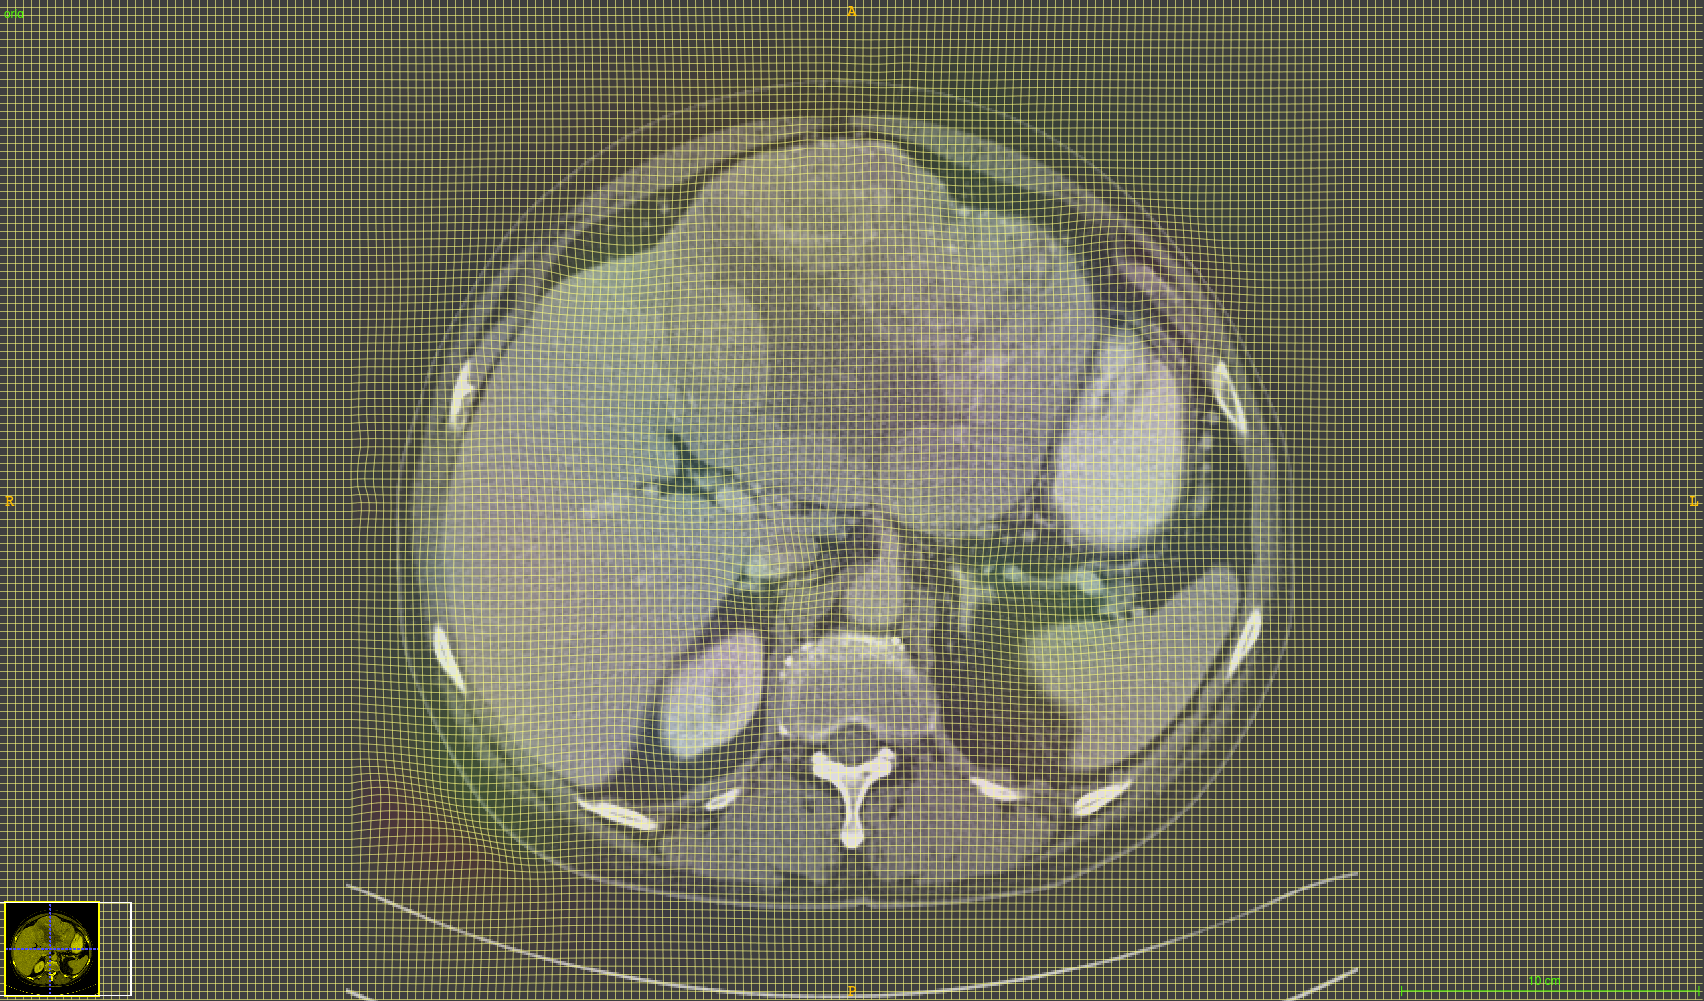
\includegraphics[width=\linewidth]{../HistologicalGradePrediction/images/TCIA_TCGA-DD-A11A_deformation_grid_slice49}
\end{minipage}

\vspace{0.8cm}
\begin{minipage}{0.7\linewidth}
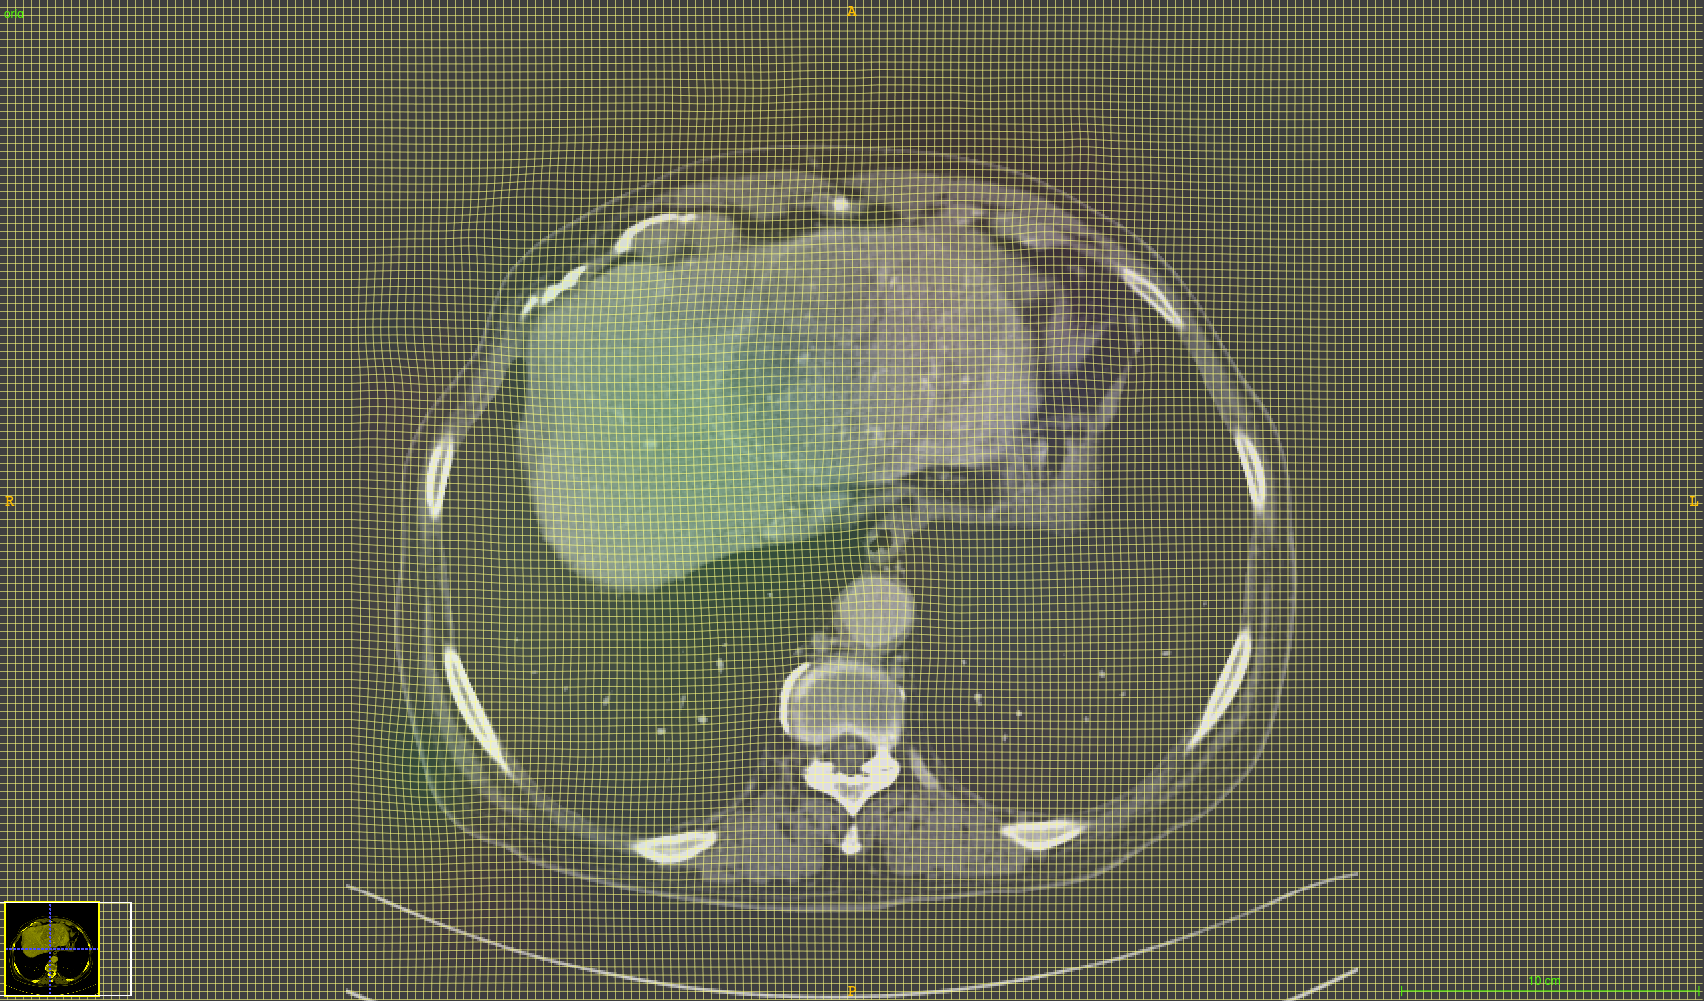
\includegraphics[width=\linewidth]{../HistologicalGradePrediction/images/TCIA_TCGA-DD-A11A_deformation_grid_slice68}
\end{minipage}
\caption{Example of deformation grids obtained after applying the registration pipeline on \lmttfont{TCIA-dB} patients}
\label{fig:deformationGridExamples}
\end{figure}
One way to assess the precision of the registration is to apply the
transformation matrix to the initial resampled \ac{ar} liver mask and to
compute the \ac{dsc} with the target \ac{pv} liver mask. When applying this
evaluation, we obtained a mean patient-wise \ac{dsc} of $ 92.8 \pm 3.8 $ between the target \ac{pv} and the registered \ac{ar} liver masks at the
end of the registration step on the \textbf{\lmttfont{TCIA-dB}}, sufficient to consider the
registration as successful when compared with those obtained by state-of-the-art
registration methods applied to the liver (where mean liver masks dices obtained after a subject-to-subject registration varied between 0.96 and 0.91 when applied to respectively the SLIVER and the LITS datasets) \cite{Zhao2019}.

The complete registration pipeline applied to the \textbf{\lmttfont{TCIA-dB}} is detailed in the table \ref{regisPipeline}.

\subsection{Automatic multiphase tumor segmentation}\label{tcia-db-unsupervised-multiphase-tumor-segmentation}

Once both the \ac{ar} and \ac{pv} volumes of the \textbf{\lmttfont{TCIA-dB}} were registered, and the
liver masks obtained, we built the second step of our cascaded
architecture, dedicated to the multiphasic tumor segmentation. In order
to train such a network, we created a multiphase (arterial and portal
venous) database where the temporal volumes of a given patient are
registered and where segmentations of both the liver and tumor regions
are available.
\textbf{\lmttfont{TheraHCC-dB}} and \textbf{\lmttfont{G-dB}} were the only two datasets containing multiphasic
images (as we can see in table \ref{xp_datasets}), however
\textbf{\lmttfont{G-dB}} initially contained ground truth annotation only for the tumors,
with segmentations performed only on the \ac{ar} phase images.
Since \textbf{\lmttfont{G-dB}} contains more cases than \textbf{\lmttfont{TheraHCC-dB}}, we have decided to
build our multiphasic tumor segmentation network on this dataset.
However in order to train a tumor segmentation network, our cascaded
architecture requires to have the liver segmentation mask as input for
the second step (as depicted in the figure \ref{CARS_DMP_Full_Fig}), therefore we had to obtain the liver segmentation
mask for the patients of the \textbf{\lmttfont{G-dB}}.

\ac{ar} and \ac{pv} volumes of the \textbf{\lmttfont{G-dB}} dataset were initially not registered so
we applied the same registration pipeline as the one used for \textbf{\lmttfont{TCIA-dB}} (see table \ref{regisPipeline}). After application of the procedure to
each patient of \textbf{\lmttfont{G-dB}}, we used the resulting transformation matrix to
transform the \ac{ar} tumor mask to the \ac{pv} space as depicted by the red and green dashed arrows in the figure \ref{fig:GDB_registration_pipeline_vertical}.


\begin{figure}[th!]
\centering
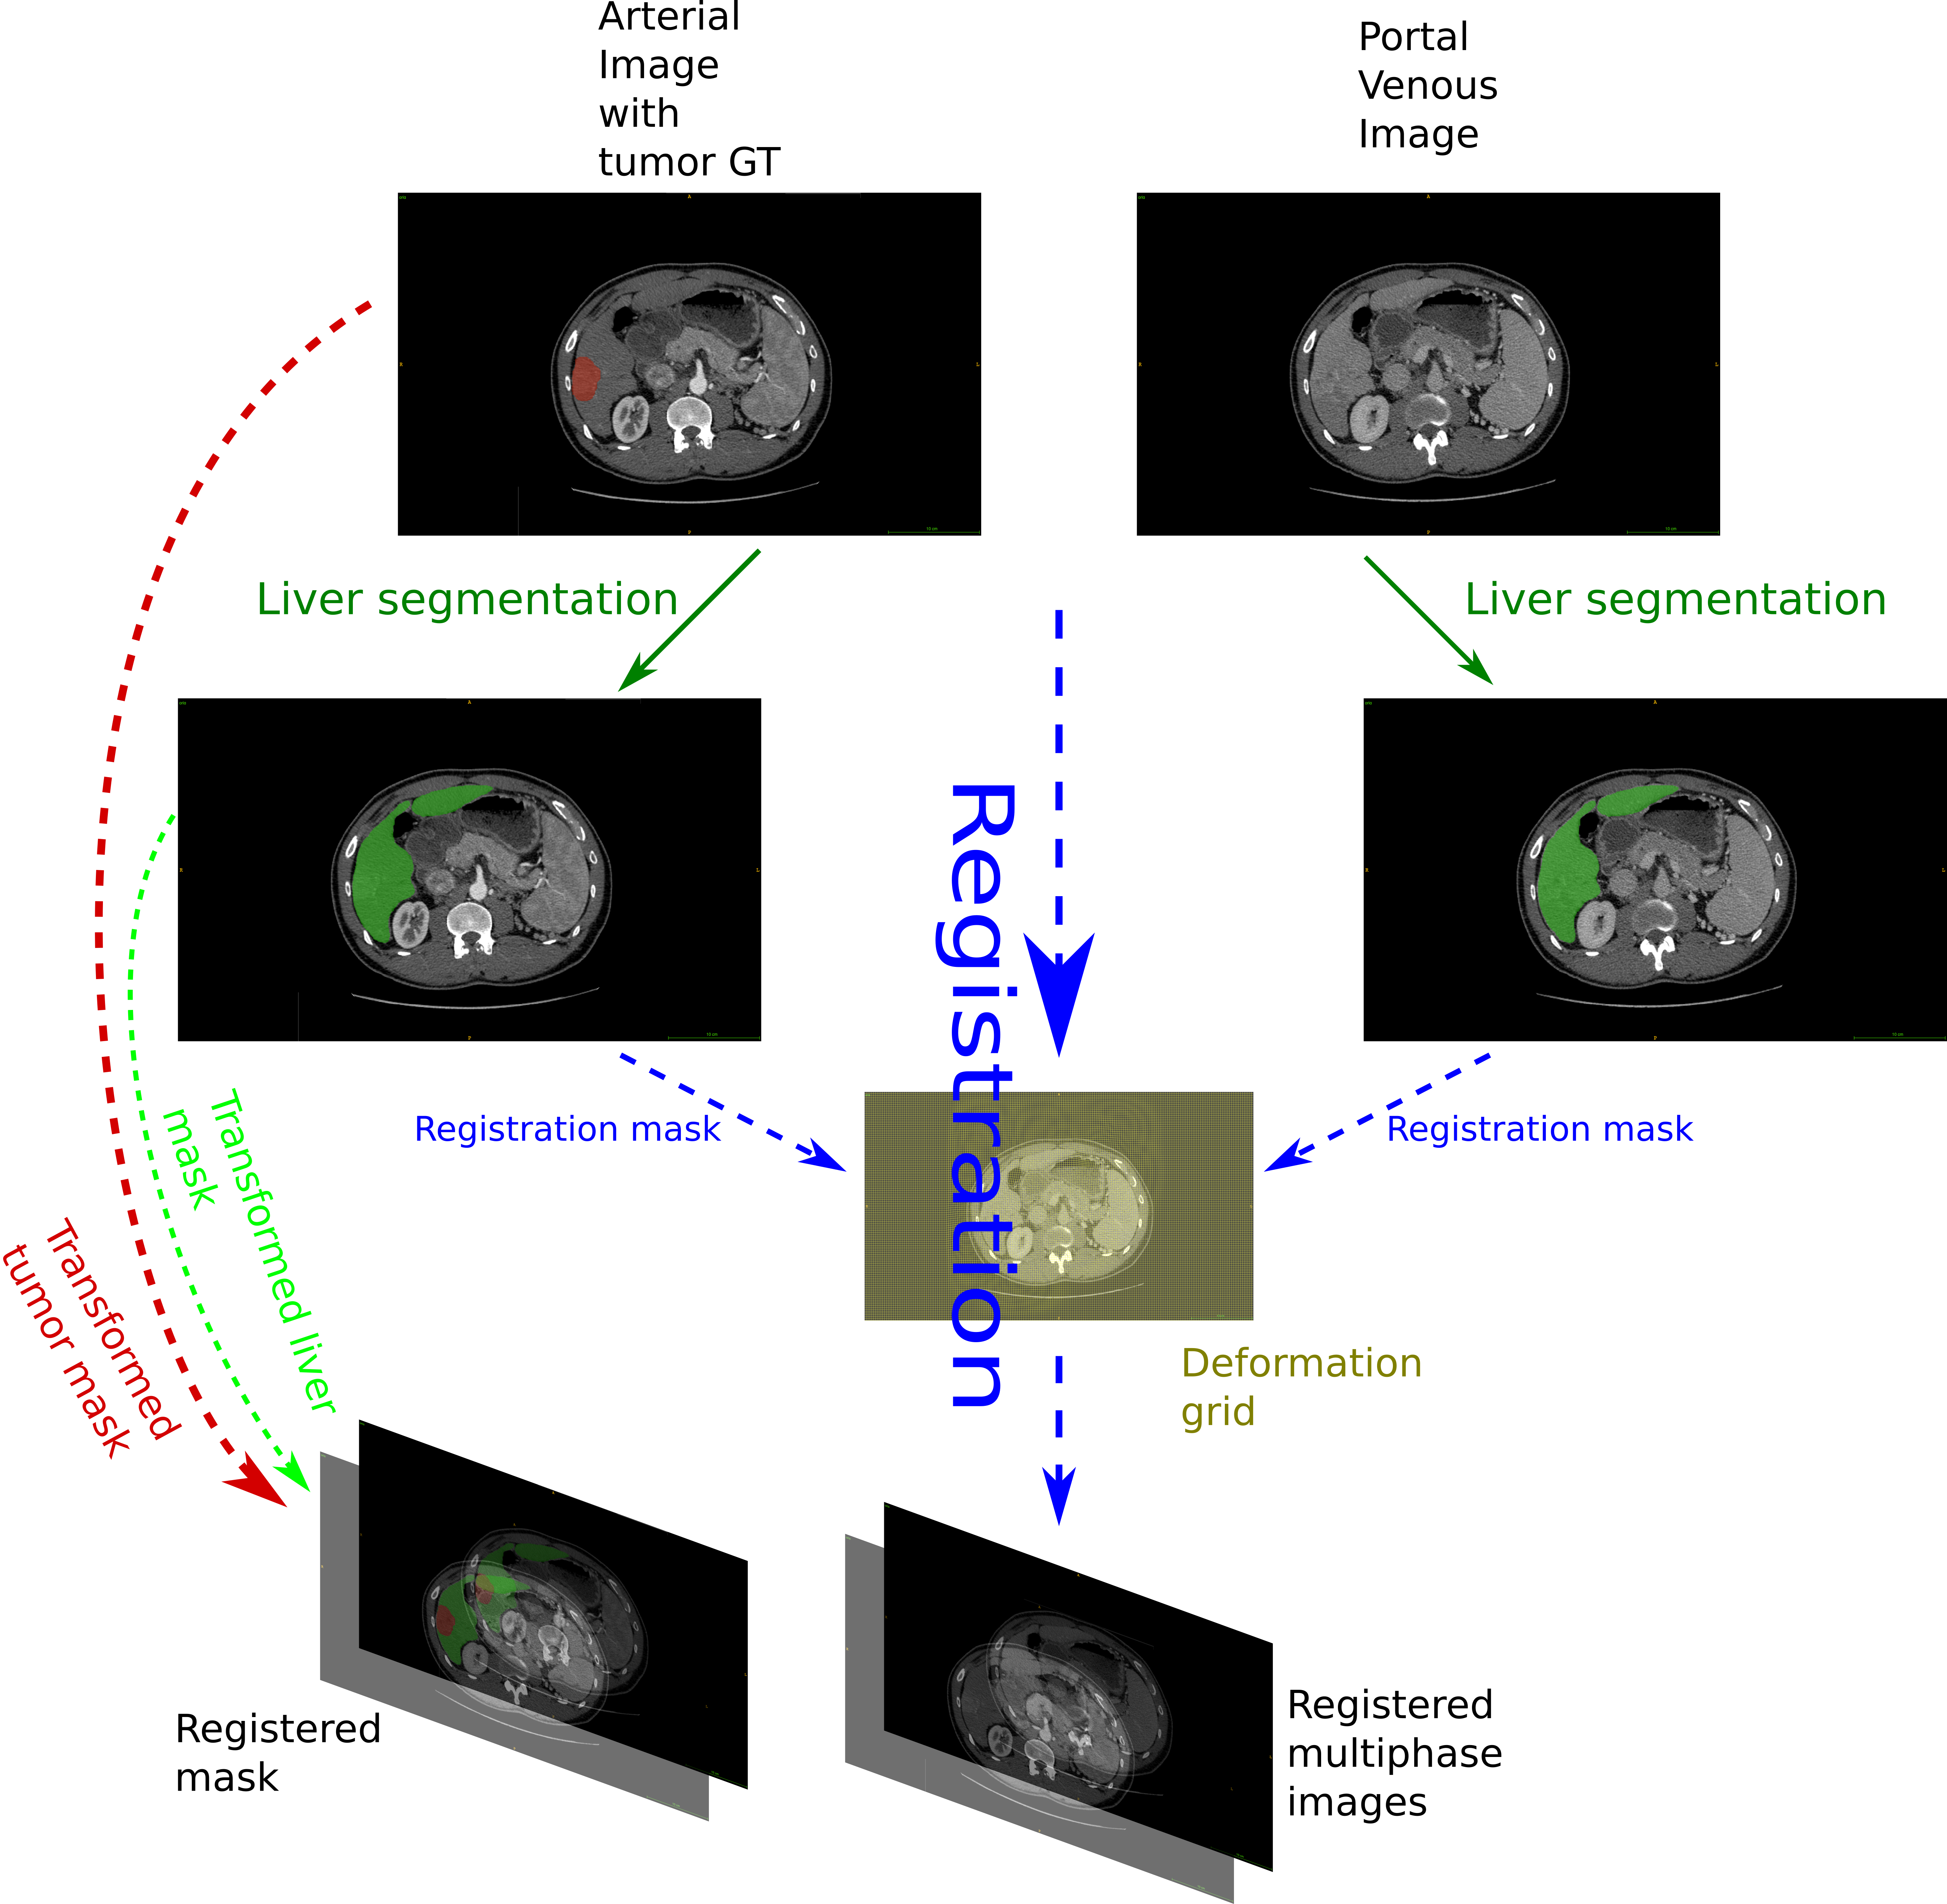
\includegraphics[width=0.9\linewidth]{../HistologicalGradePrediction/images/GDB/GDB_registration_pipeline_vertical}
\caption{Illustration of the registration pipeline applied to \textbf{\lmttfont{G-dB}}. A similar approach as the one applied to \textbf{\lmttfont{TCIA-dB}} is performed to obtain the registered multiphase images. A final step is added here to transform both the tumor and the liver masks using the registration transformation matrix (red and green dashed arrows)}
\label{fig:GDB_registration_pipeline_vertical}
\end{figure}

We then trained our multiphase tumor segmentation network using the \textbf{\lmttfont{G-dB}} as training dataset.
\textcolor{red}
{
To compare both the training (\textbf{\lmttfont{G-dB}}) and the testing (\textbf{\lmttfont{TCIA-dB}}) datasets, we achieved the same analysis as the one performed previously (see section \ref{tcia-db-unsupervised-liver-segmentation_material}).
Therefore, a medical expert was asked to evaluate both visually and quantitatively the differences between the two datasets.
To perform the visual analysis, he was asked to evaluate the type of characteristics present in both dataset, not only in the liver but also by comparing the tumors using imaging features. 
As exposed previously, \textbf{\lmttfont{TCIA-dB}} contains both large and small tumors, and the same panel of tumor sizes was present in the \textbf{\lmttfont{G-dB}} dataset, as illustrated in the figure \ref{fig:interdb_tumorSeg_tumorExamples}.
\begin{figure}[!ht]
	\begin{mdframed}[backgroundcolor=blue!50,linecolor=blue!50]
		\centering
		\begin{minipage}{0.45\linewidth}
			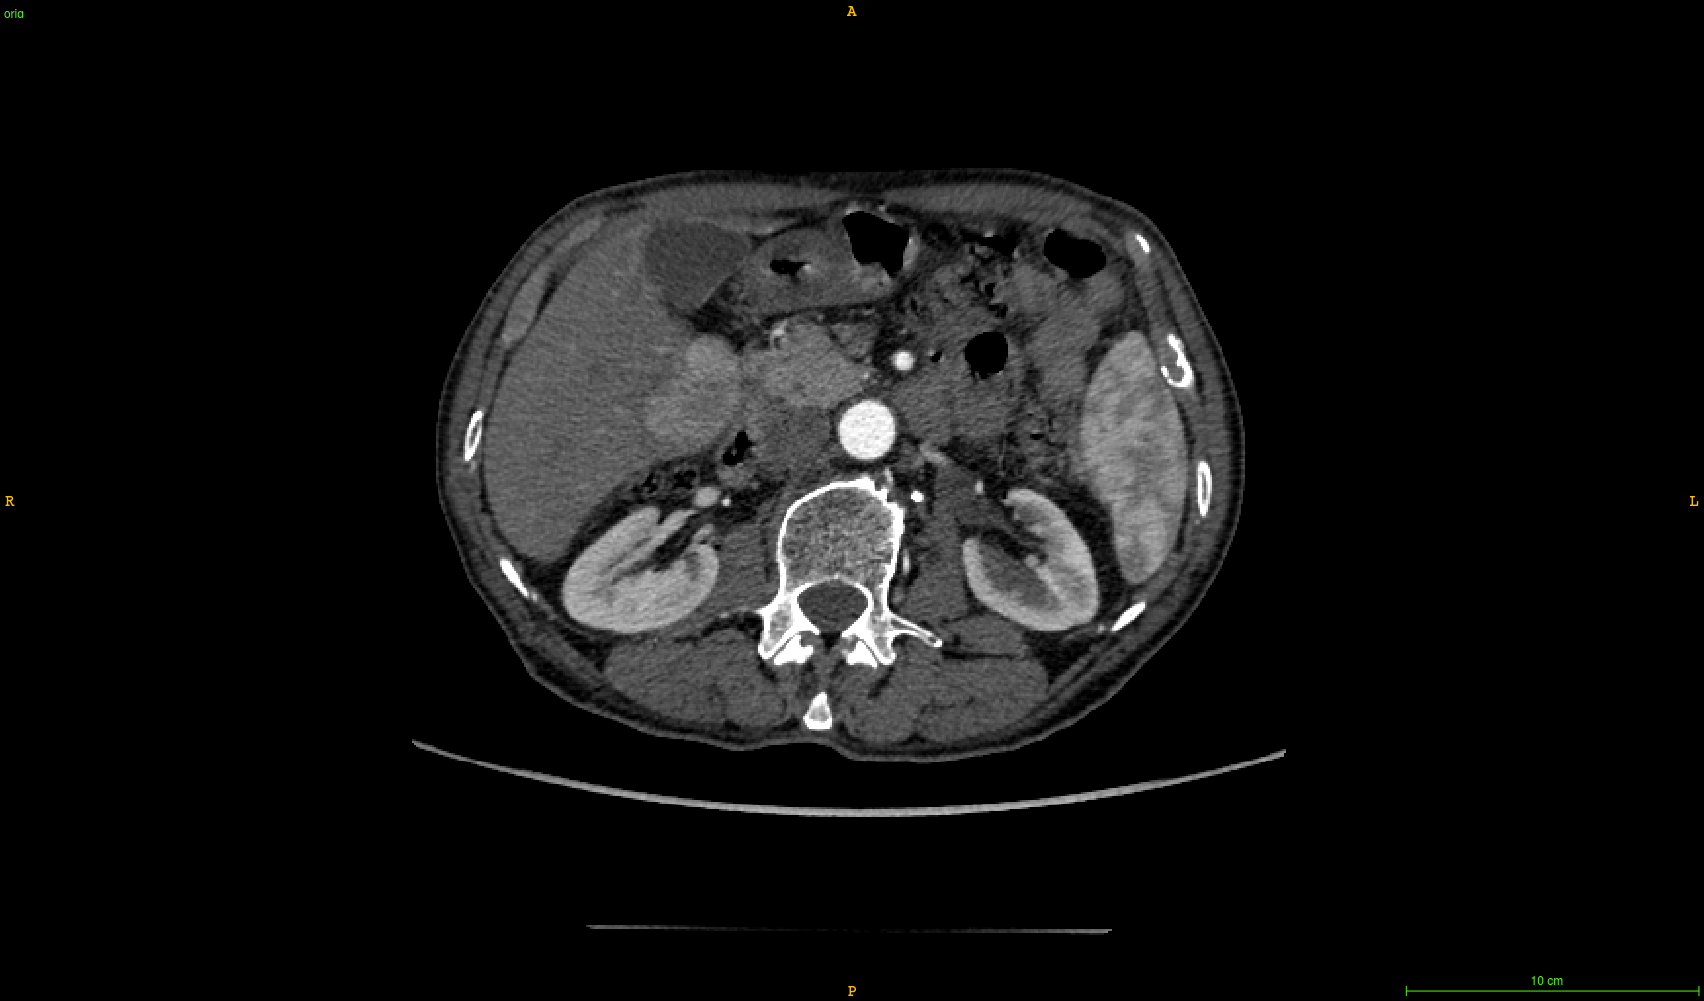
\includegraphics[width=\linewidth]{images/GDB_examplePatientSmallTumor}
		\end{minipage} \hspace{-0.1cm}
		\begin{minipage}{0.45\linewidth}
			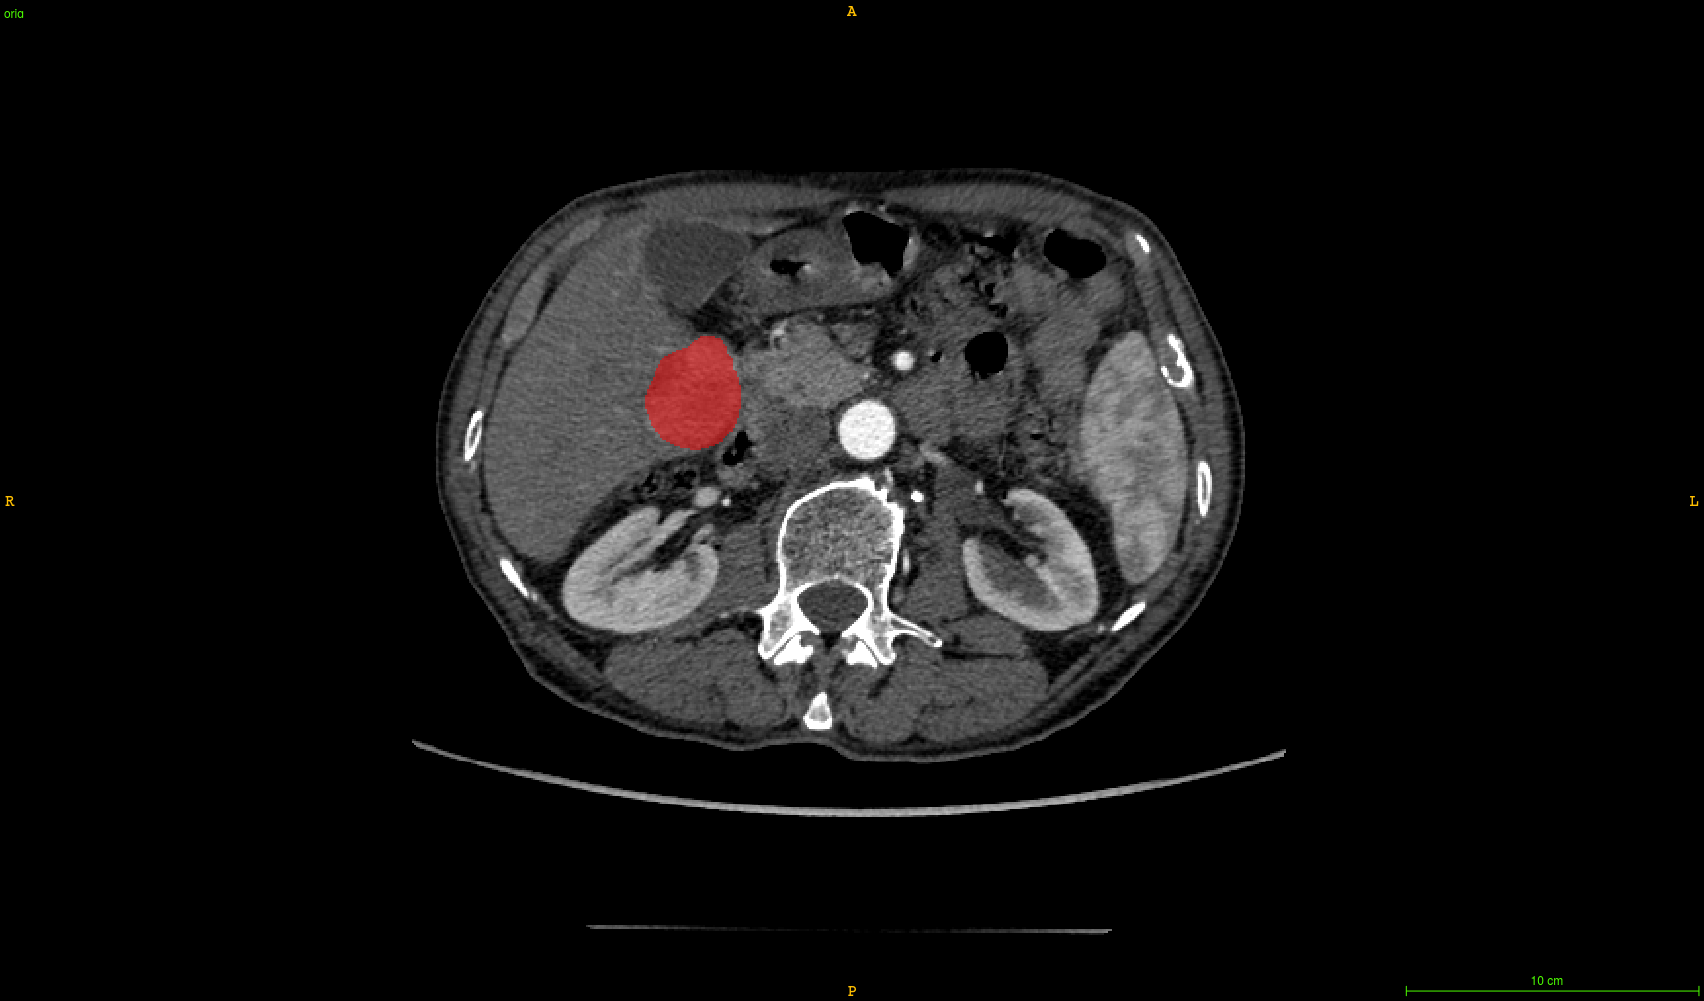
\includegraphics[width=\linewidth]{images/GDB_examplePatientSmallTumor_seg}
		\end{minipage} \\
		\begin{minipage}{0.45\linewidth}
			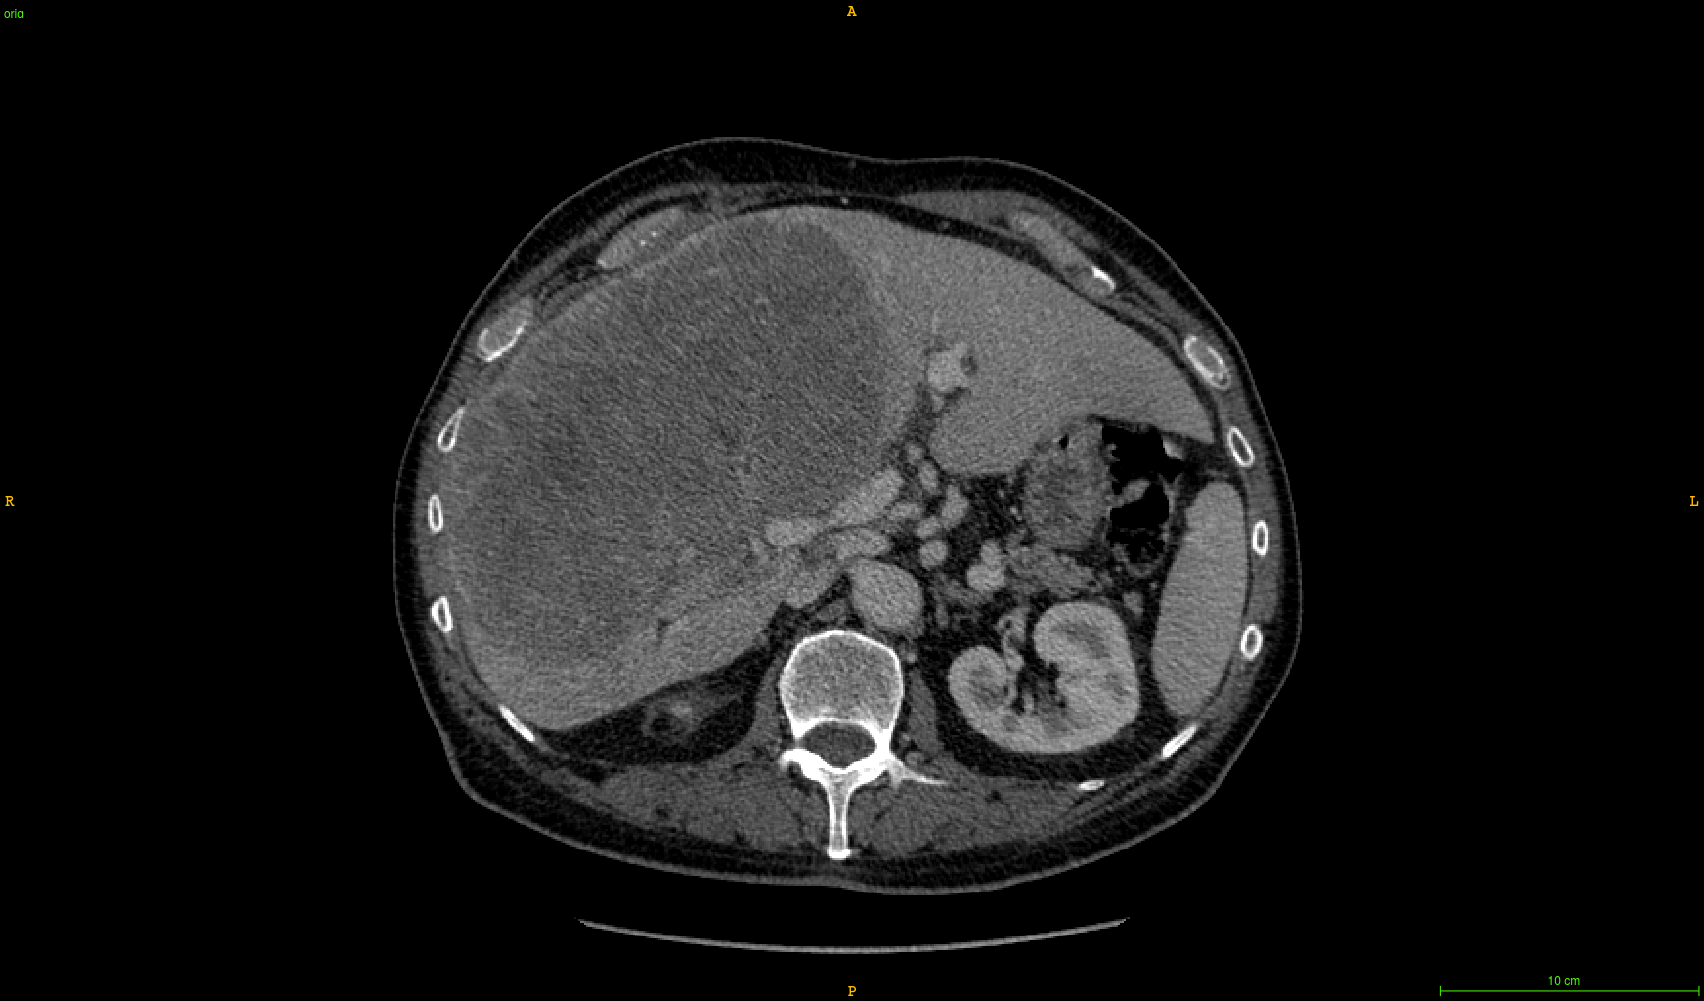
\includegraphics[width=\linewidth]{images/GDB_examplePatientLargeTumor}
		\end{minipage} \hspace{-0.1cm}
		\begin{minipage}{0.45\linewidth}
			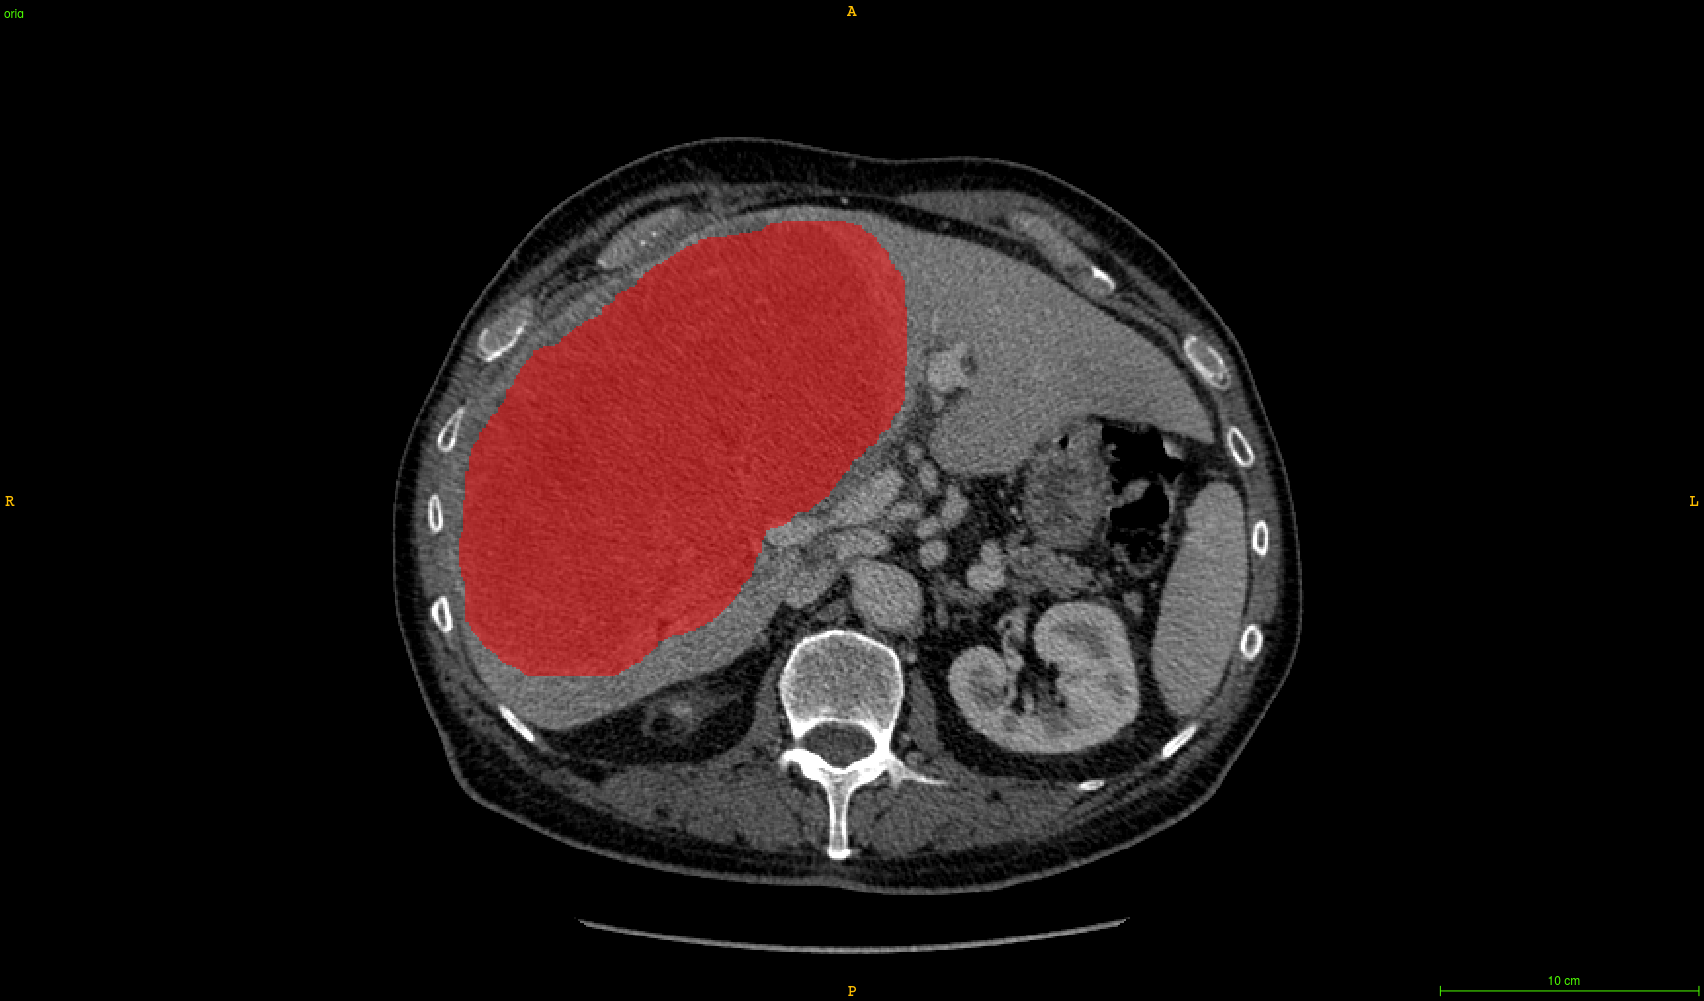
\includegraphics[width=\linewidth]{images/GDB_examplePatientLargeTumor_seg}
		\end{minipage}
	\end{mdframed}
	\caption{Example of small and large tumors from the \textbf{\lmttfont{G-dB}} images, top: small tumors, bottom: large tumors, left: raw image, left: expert segmentation.}
	\label{fig:interdb_tumorSeg_tumorExamples}
\end{figure}
Some artifacts were also found in the \textbf{\lmttfont{G-dB}} dataset, such as the presence of benign lesions, fat accumulation or other metallic artifacts in the hepatic region (see figure \ref{fig:GDb_artifacts}).
\begin{figure}[!ht]
	\begin{mdframed}[backgroundcolor=blue!50,linecolor=blue!50]
		\centering
		\begin{minipage}{0.45\linewidth}
			\includegraphics[width=\linewidth]{images/Artifacts/GDB_cyst}
		\end{minipage} \\
		\begin{minipage}{0.45\linewidth}
			\includegraphics[width=\linewidth]{images/Artifacts/GDB_fat}
		\end{minipage} \\
		\begin{minipage}{0.45\linewidth}
			\includegraphics[width=\linewidth]{images/Artifacts/GDB_metallic_artifacts}
		\end{minipage}
	\end{mdframed}
	\caption{Example of artifacts present in the \textbf{\lmttfont{G-dB}} dataset. First row depicts a patient with benign hepatic lesion (yellow arrows), second row presents liver with tracks of fat accumulation (orange arrows), whereas last row gives example of images with presence of metallic artifacts (red arrows).}
	\label{fig:GDb_artifacts}
\end{figure}
As it was the case in the \textbf{\lmttfont{TCIA-dB}} dataset, diseased livers were also present among the \textbf{\lmttfont{G-dB}} patients, as illustrated in the figure \ref{fig:GDb_diseasedLivers}.
\begin{figure}[!ht]
	\begin{mdframed}[backgroundcolor=blue!50,linecolor=blue!50]
		\centering
		\begin{minipage}{0.45\linewidth}
			\includegraphics[width=\linewidth]{images/GDB_cirrhoticPatientArrows}
		\end{minipage} \hspace{-0.1cm}
		\begin{minipage}{0.45\linewidth}
			\includegraphics[width=\linewidth]{images/GDB_cirrhoticPatientArrows_2}
		\end{minipage}
	\end{mdframed}
	\caption{Example of cirrhotic patients present in the \textbf{\lmttfont{LITS-dB}} dataset. In both images, we can see the irregular shape (cyan arrows) of the liver.}
	\label{fig:GDb_diseasedLivers}
\end{figure}
Regarding the tumor specific area, several imaging features were found in both datasets:
\begin{itemize}
\item the presence of internal arteries
\item a peritumoral enhancement
\item the presence of either smooth or non-smooth margins
\item an hypoattenuating halo surrounding the tumor
\item a high textural heterogeneity
\item a wash-in/wash-out pattern 
\end{itemize}
Images illustrated each of the mentioned features were given in the figure \textbf{TODO} \ref{fig:InterDb_imagingTraits}.
\begin{figure}[!ht]
	\begin{mdframed}[backgroundcolor=blue!50,linecolor=blue!50]
		\centering
		\begin{minipage}{0.45\linewidth}
			\includegraphics[width=\linewidth]{images/ImagingTraits/GDB_peritumoralEnhancement}
		\end{minipage} \hspace{-0.1cm}
		\begin{minipage}{0.45\linewidth}
			\includegraphics[width=\linewidth]{images/ImagingTraits/TCIA_peritumoralEnhancement}
		\end{minipage} \\
		\begin{minipage}{0.45\linewidth}
			\includegraphics[width=\linewidth]{images/ImagingTraits/GDB_smoothMargins}
		\end{minipage} \hspace{-0.1cm}
		\begin{minipage}{0.45\linewidth}
			\includegraphics[width=\linewidth]{images/ImagingTraits/TCIA_smoothMargins}
		\end{minipage} \\
		\begin{minipage}{0.45\linewidth}
			\includegraphics[width=\linewidth]{images/ImagingTraits/GDB_nonSmoothMargins}
		\end{minipage} \hspace{-0.1cm}
		\begin{minipage}{0.45\linewidth}
			\includegraphics[width=\linewidth]{images/ImagingTraits/TCIA_nonSmoothMargins}
		\end{minipage} \\
		\begin{minipage}{0.45\linewidth}
			\includegraphics[width=\linewidth]{images/ImagingTraits/GDB_halo}
		\end{minipage} \hspace{-0.1cm}
		\begin{minipage}{0.45\linewidth}
			\includegraphics[width=\linewidth]{images/ImagingTraits/TCIA_halo}
		\end{minipage} \\
	\end{mdframed}
	\caption{Examples of tumor characteristic imaging traits relative to the tumor border present in both training and test datasets. Left: \textbf{\lmttfont{G-dB}} images, right: \textbf{\lmttfont{TCIA-dB}} images. First row: peritumoral enhancement, which can be defines by the presence of a detectable region of enhancement adjacent to the tumor border in the arterial phase. Second and third rows: illustration of the tumor margin, that can be categorized as a smooth margin (second row) when facing nodular tumors with smooth contours or as non-smooth margin (third row) when facing non-nodular tumors with an irregular margin with budding portions at the periphery in both \ac{ar} and \ac{pv} images. Bottom row: hypoattenuating halo, defined as a rim of hypoattenuation partially or completely circumscribing the tumor on perituromal \ac{pv} images. }
	\label{fig:InterDb_imagingTraits}
\end{figure}
\begin{figure}[!ht]
	\begin{mdframed}[backgroundcolor=blue!50,linecolor=blue!50]
		\centering
		\begin{minipage}{0.45\linewidth}
			\includegraphics[width=\linewidth]{images/ImagingTraits/GDB_internalArteries}
		\end{minipage} \hspace{-0.1cm}
		\begin{minipage}{0.45\linewidth}
			\includegraphics[width=\linewidth]{images/ImagingTraits/TCIA_internalArteries}
		\end{minipage} \\
		\begin{minipage}{0.45\linewidth}
			\includegraphics[width=\linewidth]{images/ImagingTraits/GDB_texturalHeterogeneity}
		\end{minipage} \hspace{-0.1cm}
		\begin{minipage}{0.45\linewidth}
			\includegraphics[width=\linewidth]{images/ImagingTraits/TCIA_texturalHeterogeneity}
		\end{minipage} \\
	\end{mdframed}
	\caption{Example of tumor characteristic imaging traits, relative to the inner part of the tumor, present in both training and test datasets. Left: \textbf{\lmttfont{G-dB}} images, right: \textbf{\lmttfont{TCIA-dB}} images. Top row: internal arteries, defined by the persistence of discrete arterial enhancement within the tumor in the \ac{ar} phase. Bottom row: high textural heterogeneity.}
	\label{fig:InterDb_imagingTraits2}
\end{figure}
\begin{figure}[!ht]
	\begin{mdframed}[backgroundcolor=blue!50,linecolor=blue!50]
		\centering
		\begin{minipage}{0.45\linewidth}
			\includegraphics[width=\linewidth]{images/ImagingTraits/GDB_washin}
		\end{minipage} \hspace{-0.1cm}
		\begin{minipage}{0.45\linewidth}
			\includegraphics[width=\linewidth]{images/ImagingTraits/TCIA_washin}
		\end{minipage} \\
		\begin{minipage}{0.45\linewidth}
			\includegraphics[width=\linewidth]{images/ImagingTraits/GDB_washout}
		\end{minipage} \hspace{-0.1cm}
		\begin{minipage}{0.45\linewidth}
			\includegraphics[width=\linewidth]{images/ImagingTraits/TCIA_washout}
		\end{minipage}
	\end{mdframed}
	\caption{Example of specific wash-in/wash-out trait present in both training and test datasets. Left: \textbf{\lmttfont{G-dB}} images, right: \textbf{\lmttfont{TCIA-dB}} images.
	Wash-in is defined as an enhancement of the lesion of the arterial phase higher than the one of the liver parenchyma, whereas the wash-out is defined as a lesion hypodense/hypointense compared to the liver parenchyma on the portal venous and/or delayed phases.}
	\label{fig:InterDb_imagingTraits3}
\end{figure}
The same quantitative analysis as previously was performed (see section \ref{tcia-db-unsupervised-liver-segmentation_material}), with the placement of 5 ROIs in randomly chosen patients of both the training (\textbf{\lmttfont{G-dB}}) and the testing (\textbf{\lmttfont{TCIA-dB}}) datasets. ROIs were placed in the liver parenchyma, the air, the spleen, the bone and the aorta. These areas were chosen mainly to detect potential cirrhotic patients in both datasets, as illustrated in the figure \ref{fig:cirrhoticPatPlot} , and to assess the homogeneity for the given phases among the different datasets, as depicted in the figure \ref{fig:gdbAortaPlot}. 
\begin{figure}[!ht]
	\begin{mdframed}[backgroundcolor=blue!50,linecolor=blue!50]
		\centering
		\includegraphics[width=0.6\linewidth]{images/Gdb_TCIA_cirrhosisPlot}
		\caption{Histogram representing the distribution of the difference between parenchyma and spleen intensities for the patients of  \textbf{\lmttfont{G-dB}} dataset (green) and the  \textbf{\lmttfont{TCIA-dB}} dataset (blue). A difference higher than 18.5 HU (black vertical line) can be a sign of cirrhosis.
		}
		\label{fig:cirrhoticPatPlot}
	\end{mdframed}
\end{figure}
\begin{figure}[!ht]
	\begin{mdframed}[backgroundcolor=blue!50,linecolor=blue!50]
		\centering
		\includegraphics[width=0.6\linewidth]{images/AortaParPlot_Gdb}
		\caption{Mean aorta intensity vs mean liver parenchyma intensity. Each point represents one volume. We can see a clear separation between arterial (green dots) and portal venous (red crosses) volumes for both the \textbf{\lmttfont{G-dB}} and the \textbf{\lmttfont{TCIA-dB}} patients. We can however notice a higher heterogeneity among the mean parenchyma intensity in the \textbf{\lmttfont{TCIA-dB}} dataset, which could be a sign of standardize acquisition settings for the \textbf{\lmttfont{G-dB}}.
		}
		\label{fig:gdbAortaPlot}
	\end{mdframed}
\end{figure}
}

We then fused the liver and the tumor masks to obtain a multiclass
segmentation mask that can fit both the \ac{pv} and the registered \ac{ar} volumes, as depicted in the figure \ref{fig:gDbRegisteredPatient}.

\begin{figure}[ht!]
	\centering
	\begin{minipage}{0.45\linewidth}
		\includegraphics[width=\linewidth]{../HistologicalGradePrediction/images/GDB/GDB_Pat77_slice261_AR_TumorPred}
	\end{minipage} \hspace{-0.1cm}
	\begin{minipage}{0.45\linewidth}
		\includegraphics[width=\linewidth]{../HistologicalGradePrediction/images/GDB/GDB_Pat77_slice261_AR_liverTumorPred}
	\end{minipage} \\
	\begin{minipage}{0.45\linewidth}
	\includegraphics[width=\linewidth]{../HistologicalGradePrediction/images/GDB/GDB_Pat77_slice261_raw_PV}
	\end{minipage} \hspace{-0.1cm}
	\begin{minipage}{0.45\linewidth}
	\includegraphics[width=\linewidth]{../HistologicalGradePrediction/images/GDB/GDB_Pat77_slice261_PV_liverTumorPred}
	\end{minipage}
	\caption{Example of a patient from \textbf{\lmttfont{G-dB}}, obtained after enhancing the dataset with our semantic segmentation network and our registration pipeline. Top row: \ac{ar}\_registered volume with original tumor expert segmentation, bottom row: \ac{pv}\_volume, left: original raw volumes, right: segmentation mask overlay where the parenchyma is obtained through our segmentation pipeline and the tumor was initially delineated by an expert then transformed to fit the target volume space.}
	\label{fig:gDbRegisteredPatient}
\end{figure}


We were able thanks to our cascaded architecture and a robust liver
segmentation network to provide additional annotations to the volumes present in \textbf{\lmttfont{G-dB}} that
originally contained only experts annotations for the tumor area on \ac{ar} volumes.

Once a complete database where both the liver and the tumor segmentation
masks were available, and where \ac{ar} and \ac{pv} volumes were registered, we
trained a robust multiphase tumor segmentation network.

We trained both a \pplfont{DMP-Tumor} and a \pplfont{MPF-Tumor} segmentation network on the
registered \textbf{\lmttfont{G-dB}} dataset, and evaluated them on \lmttfont{TCIA-dB} which
contained expert tumor annotations. We evaluated both \pplfont{DMP} and \pplfont{MPF}
architectures since no statistical differences were available when
comparing results obtained for the tumor segmentation in our previous
work on \textbf{\lmttfont{TheraHCC-dB}} \cite{Ouhmich2019}.

After training both architectures with
the same parameters, we obtained a mean patient-wise \ac{dsc} of $ 73.2 \pm 20.6 $ with \pplfont{MPF}
architecture versus $ 64.9 \pm 27.2 $ when using the \pplfont{DMP} when evaluating the
models on the \textbf{\lmttfont{TCIA-dB}} patients. An example of prediction on the \textbf{\lmttfont{TCIA-dB}} is
depicted in figure \ref{fig:TCIAMultiphaseTumorPred}. 
\textcolor{red}
{
Event though the accuracy tends to be very high, we found some cases where the tumor segmentation contains some false positives, as illustrated in the figure \ref{fig:GDB_TumorMisSeg}.
\begin{figure}[!ht]
	\begin{mdframed}[backgroundcolor=blue!50,linecolor=blue!50]
		\centering
		\begin{minipage}{0.3\linewidth}
			\includegraphics[width=\linewidth]{images/MisSegmentations/TCGA-DD-A1ED_slice41_raw}
		\end{minipage} \hspace{-0.1cm}
		\begin{minipage}{0.3\linewidth}
			\includegraphics[width=\linewidth]{images/MisSegmentations/TCGA-DD-A1ED_slice41_raw_windowed}
		\end{minipage} \hspace{-0.1cm}
		\begin{minipage}{0.3\linewidth}
			\includegraphics[width=\linewidth]{images/MisSegmentations/TCGA-DD-A1ED_slice41_TumorPrediction}
		\end{minipage} \vspace{0.3cm}
		\begin{minipage}{0.45\linewidth}
			\includegraphics[width=\linewidth]{images/MisSegmentations/TCGA-DD-A4NK_slice75_raw}
		\end{minipage} \hspace{-0.1cm}
		\begin{minipage}{0.45\linewidth}
			\includegraphics[width=\linewidth]{images/MisSegmentations/TCGA-DD-A4NK_slice75_TumorPrediction}
		\end{minipage}
	\end{mdframed}
	\caption{Examples of tumor mis-segmentation.
	In both cases, enhanced parts of the liver have been wrongly considered as being tumoral. Top row: the raw images has been windowed in such a case that enhanced part are easily visible (middle image). Only the bottom ROI correctly belong to the tumor, whereas the top ROI is a false positive (third image). The bottom row depicts an other example where the segmented areas corresponds to a false positive.}
	\label{fig:GDB_TumorMisSeg}
\end{figure}
}



\begin{figure}
	\begin{minipage}{0.3\linewidth}
		\includegraphics[width=\linewidth]{../HistologicalGradePrediction/images/image13.png}
	\end{minipage} \hspace{0.1cm}
	\begin{minipage}{0.3\linewidth}
		\includegraphics[width=\linewidth]{../HistologicalGradePrediction/images/image10.png}
	\end{minipage} \hspace{0.1cm}
	\begin{minipage}{0.3\linewidth}
		\includegraphics[width=\linewidth]{../HistologicalGradePrediction/images/image7.png}
	\end{minipage}
	\caption{Example of an image from the \textbf{\lmttfont{TCIA-dB}}, with the obtained predicted tumor
	segmentation using the \pplfont{MPF-Tumor} segmentation network (left: raw,
	middle: expert annotation, right: obtained segmentation)}
	\label{fig:TCIAMultiphaseTumorPred}
\end{figure}


Those results obtained on an external dataset tend to demonstrate a satisfactory precision
of the tumor segmentation when training a cascaded architecture with a
sufficient number of cases.
We retained the \pplfont{MPF-Tumor} segmentation network since it performed
significantly better than the \pplfont{DMP} one ($ p = 0.02 $ using a Wilcoxon signed
paired rank test on the patient-wise \ac{dsc}).
We confirmed the benefit of the cascaded architecture since these results
were obtained using an architecture where the first network was trained
on \textbf{\lmttfont{LITS-dB}} and the second on \textbf{\lmttfont{G-dB}}. We were also able to use
a monophase network for the first step and a multiphasic network for the
second.
This work proved the ability of deep learning (semantic segmentation
network) combined with image processing (registration) to enhance and
complete weakly annotated databases (both \textbf{\lmttfont{TCIA-dB}} and \textbf{\lmttfont{G-dB}} were
enhanced in the same way).

%Finally, we decided to keep only two stages in our cascaded architecture
%since the only available dataset with expert necrosis annotation was the
%\lmttfont{TheraHCC-dB}, containing only 7 patients. This small amount of cases
%combined with the design of \lmttfont{TheraHCC-dB} (only sparse slices are
%annotated across the volume) might not be enough to precisely
%differentiate between the active and the necrotic part of the lesions on
%unseen cases. Moreover, the necrosis segmentation appears to be more
%sensitive than the tumor segmentation, especially because the necrosis
%requires separate annotations in each phase (in case of \ac{ar} and \ac{pv} volumes) since necrotic tissues will respond differently to the evolution of contrast medium.



\section{Automatic histological grade prediction}

\subsection{Introduction}\label{introduction}

The main goal of our work is to use imaging features to better characterize the liver cancers.
We decided to extract relevant imaging features from our multiphase cascaded semantic segmentation
to perform the prediction of histological grade.
The prediction of the histological grade of the tumor was rarely studied, since only one study
used deep learning tools to perform this task but with MR images as
input \cite{Yang2019} (see section \ref{ct-and-mr-imaging} to get more details on both modalities and our choice to focus on \ac{ct} imaging).
Indeed, this task appears to be more challenging than previous \ac{dlr}
liver-related work where either the type of \ac{fll} or the treatment
response (such as the recurrence) were predicted (see section \ref{deep-learning-radiomics}), however, being able to perform such a prediction could highly improve the automatic characterization of liver tumors, as seen in the section \ref{histological-hcc-grading-systems}.
We will now review the only study in the literature that addressed the
problem of predicting the histological grade of \ac{hcc}s through a \ac{dl}
architecture with medical images, before presenting our own automatic \ac{dl}
pipeline.\\
We now present our contribution.

\subsection{Related work}\label{dlr-based-study-to-predict-the-histological-hcc-grade}

To our knowledge, only one study tackled the problem of estimating the
histological grade of \ac{hcc}s using a \ac{dl} architecture, but with MR images
as input \cite{Yang2019}.

Yang et al. incorporated 42 patients suffering from \ac{hcc} in their study,
resulting in a total of 51 \ac{hcc}s. Each lesion was analyzed by 2
experienced pathologists who estimated their histological grade after
microscopic examination (the lesions were classified as well, moderately
and poorly differentiated, following the WHO classification system \cite{20113051318}) .
The extracted tissues were obtained through either biopsy (12 patients)
or after surgical removal (2 liver transplants and 28 liver resection).
All the 42 patients underwent pre-operative multiphasic MR imaging
examinations and images were available at 5 different phases
(precontrast, late arterial, portal venous, equilibrium and delayed
phases). They obtained a dataset composed of 9 well, 7 poorly and 35 moderately
differentiated \ac{hcc}s.

For each patient, a \ac{roi} was placed by one expert at the maximal axial
cross-sectional area to entirely cover the tumor. The \ac{roi} was
copied in the 2 slices above and below the chosen one, to obtain a 3D
volume. Intensities of each volume were normalized and 4D tensors were
created for each patient so that each tensor had a $ 32\times32\times5\times5 $ shape
($ 32\times32 $ corresponding to the resampled axial \ac{roi} dimension, the third
dimension being the number of retained slices, and the last dimension being the
dynamic temporal evolution of the \ac{roi} with the 5 phases).

The used architecture is depicted in the figure \ref{fig:Yang2019_Figure2_MCF-3DCNN}. It first splits the 4D
tensors into 5 3D objects so that each slice is treated separately. Each
3D volume was then processed by 2 convolutional, 2 max pooling and 1
fully connected layer. The features of each slice were then
concatenated, before a second fully connected layer followed by a dense
layer with a softmax activation function outputs the probability of
belonging to each one of the three classes (well, moderately or poorly differentiated).

\begin{figure}[th!]
\centering
\includegraphics[width=0.7\linewidth]{../HistologicalGradePrediction/images/Yang2019_Fig2}
\caption{MCF-3DCNN architecture as detailed by \textbf{©Yang et al. \cite{Yang2019}}}
\label{fig:Yang2019_Figure2_MCF-3DCNN}
\end{figure}


During the training process, they implemented a label-shuffling method
to overcome the problem of imbalanced data. Furthermore, to avoid the
effect of overfitting, they trained their network with augmented data
(original images were transposed, rotated, and flipped), a learning rate
reduction and the addition of dropout (rate = 0.5).
Using their architecture they were able to correctly classify the \ac{hcc}s
into the 3 differentiation groups with a mean accuracy of \textbf{74\%}.\\
Their study however suffers from a lot of limitations such as the
reduced size of the cohort, the imbalanced data and the fact that the
analysis was only performed in a manually drawn \ac{voi}.\\
We have decided to tackle the same issue, but we implemented a fully
automatic pipeline where both the segmentation and the grade prediction
steps were performed by \ac{dl} networks.


\subsection{Prediction of the histological grade}\label{prediction-of-the-histological-grade-on-tcia-db}

In order to perform the prediction of the histological grade, our idea
is to use the imaging features retained for the liver tissue
segmentation, especially those used to segment tumoral structures.
We believe that one easy way to extract relevant imaging features is to
use those retained by the semantic segmentation networks, thus the
better the accuracy regarding the semantic segmentation of the liver
tissues, the more accurate the histological grade prediction will be.
As explained previously, we proved that a cascaded architecture combined
with the use of temporal contrast enhanced images allows a better
delineation of liver tissues. We therefore proved that the designed cascaded architecture can be applied to provide missing annotations into weakly annotated datasets such as \textbf{\lmttfont{TCIA-dB}}.
It has been proven that using temporal information can improve the accuracy of the grade prediction, by exploiting the wash-in wash-out specific features \cite{Okamoto2012}.
To conduct our \ac{dlr} study, we first performed a multiphasic
semantic segmentation of the \textbf{\lmttfont{TCIA-dB}}, before predicting the
histological grade.
After obtaining the final cascaded architecture, we built our network dedicated to the
histological grade prediction.
\textcolor{red}
{We finally performed the prediction of the histological grade using the \ac{hcr} features computed on both the AR, the PV and the [PV - AR] volume \footnote{As a way to represent the dynamic within the same volume.}, using either the expert ground truth annotations or the output of our multiphase tumor semantic segmentation network as segmentation mask.}
\textbf{\lmttfont{TCIA-dB}} contains images from 18 patients, where 9 were diagnosed with a
grade 3 (G3), 7 with a grade 2 (G2) and 2 with a grade 1 (G1). In order
to obtain a balanced training dataset, it has been decided to split them
into two groups, the first containing G1 and G2 patients, and the second containing G3 patients, as it has been done previously in the literature since G2
was considered as being closer to G1 than to G3 \cite{Han2013,Zucman-Rossi2015}. Patients from the first group (G1 and G2) were considered as
having a low grade (LG), whereas those from the second group have a high
grade (HG).

\subsubsection{HCR features-based experiments}
\textcolor{red}
{
We first performed the prediction of the histological grade using the \ac{hcr} features.
To perform the prediction of the histological grade, we have decided to extract features from either the AR or the PV volume.
Once the features extracted, we built a logistic regression model to select the relevant features and perform the prediction.
Traditionally, the radiomics features are computed in a manually-defined ROI. We therefore decided to compare the accuracy of our model when using either the expert ground truth segmentation, or the predicted ROI obtained by our semantic segmentation network.
It is difficult, or even impossible in the current \ac{hcr}-paradigm workflow to extract dynamic features, since by definition, most of the features are computed in a 2D or 3D fashion. 
In order to investigate the value brought by the dynamic information, we have decided to compute the features on a so-called \textit{perfusion} volume, where each voxel intensity corresponds to the difference between the \ac{pv} and the registered AR volume. An illustration of the process to obtain the perfusion volume is given in the figure \ref{fig:perfusion}
\begin{figure}
\centering
\includegraphics[width=0.7\linewidth]{Contributions/images/perfusion}
\caption{Left: Portal venous image, middle: registered AR image, right: perfusion image where each pixel's intensity is obtained by computing the difference between its PV and its AR intensity.}
\label{fig:perfusion}
\end{figure}
We performed a 9-fold CV training so that each patient is present at least once in the testing set. We presented the accuracy of the model in terms of how many patients were correctly classified in each of the fold. Results are given in the table \ref{tab:hcrGrade}

\begin{table}[!htp]\centering
\caption{\textbf{TODO}}\label{tab:hcrGrade}
\scriptsize
\begin{tabular}{lrrrrrr}\toprule
\multicolumn{3}{c}{Settings} &\multicolumn{3}{c}{Accuracy} \\\cmidrule{1-6}
Image type &Features Type &Tumor Segmentation &input = AR &input = PV &input = Perfusion \\\midrule
Original &1st order + shape + GLM > &0.72 &0.77 &0.72 \\
Original + Filtered (Log) &1st order + shape + GLM > &0.72 &0.83 &0.94 \\
Original + Filtered (Log) + Wavelet &1st order + shape + GLM > &0.66 &0.66 &0.66 \\
Original &1st order + shape + GLM &predicted &0.72 &0.77 &0.83 \\
Original + Filtered (Log) &1st order + shape + GLM &predicted &0.66 &0.66 &0.56 \\
Original + Filtered (Log) + Wavelet &1st order + shape + GLM &predicted &0.61 &0.61 &0.61 \\
\bottomrule
\end{tabular}
\end{table}
}

\subsubsection{DLR features-based experiments}

As explained previously, to train a network dedicated to predict the
histological grade, we have decided to focus on what we called the
relevant imaging semantic features.
We therefore extracted the features from the second network of our
cascaded architecture, to focus on the temporal behavior of the tumor.

The retained network (\pplfont{MPF-Tumor} architecture as illustrated in the figure \ref{CARS_MPF_Full_Fig}) is made of 2 classical U-Net networks, where each
one takes either the \ac{ar} or the \ac{pv} image as input. We believe
that the compressed information present in the bottleneck part of the
network can be sufficient to encode the useful information present in the
image (the U-Net will work as an auto-encoder for the semantic information). Therefore, we extracted for each patient of the \textbf{\lmttfont{TCIA-dB}}, this
encoded information in a slice-wise manner, represented by two $ 32\times32\times512 $
features cubes (one per phase in the \pplfont{MPF-Tumor} architecture) per slice
as depicted in the figure \ref{fig:MPF_Features_Selection}.


\begin{figure}[th!]
\centering
\includegraphics[width=0.95\linewidth]{../HistologicalGradePrediction/images/MPF_Features_Selection}
\caption{Red and blue areas correspond to the bottleneck part of the U-Net
network where the features extraction is performed. Each image is then
represented as a $ 32\times32\times512 $ features cube.}
\label{fig:MPF_Features_Selection}
\end{figure}


Before applying the extraction of the features, we normalized
the dimension of the different volumes of the dataset, so that each
voxel measures $ 0.68\times0.68 $mm in the axial plane (because it corresponds to
the resolution of the images used to train our semantic segmentation
network), and that the volumes have a 2.5mm z-spacing (corresponding to the
spacing of the majority of the \ac{pv} volumes in \textbf{\lmttfont{TCIA-dB}}).

We finally built an architecture responsible for the grade prediction.
We focused only on the centrally located tumor slices, since the
histological grade corresponds to a measurement of the evolution of the
disease, which tends to have more physiological effects at the center of
the tumor. Centrally located slices will therefore exhibit the highest
grade for a given patient.

Therefore, a slice-wise architecture was built, first because the
features were computed in a slice-wise manner and second because the
histological grade tends to be heterogeneous in the lesion, meaning that
a slice-wise approach allows us to give a finer prediction to find
potential areas with a more advanced disease.


\begin{figure}[th!]
\centering
\includegraphics[width=0.9\linewidth]{../HistologicalGradePrediction/images/gradpredictionArchitecture}
\caption{Slice-wise histological grade prediction using both \ac{ar} and \ac{pv} retained semantic imaging features}
\label{fig:gradpredictionArchitecture}
\end{figure}



The architecture depicted in the figure \ref{fig:gradpredictionArchitecture} works as a dimensionality
reduction algorithm, where the first 1D convolutional layers are dedicated to
reduce the number of features initially present ($ 32\times32\times512 $). The
dimensionality reduction step is performed for each phase separately,
before the remaining features are combined (simple addition in the
features space).
A final dense layer takes the remaining features as input and computes
the probability of belonging to each class thanks to a softmax activation
function (LG vs HG).

When training the network, we decided to consider that each
centrally-located tumor slice of a given patient will have a higher
probability of exhibiting the highest grade, which in this case
corresponds to the observed patient-wise grade (ES1954 histological grading system \cite{EdmondsonHA1954}).

Knowing the composition of \textbf{\lmttfont{TCIA-dB}} (9 high grade patients vs 9 low
grade ones), we performed a 9-fold CV training, so that each patient is
at least present once in the testing set, and so that the training and
the test sets contains both the same number of patients per
class (7 patients from each class in the training set and 1 patient from
each class in the testing set).

After testing several combinations for the hyperparameters, we
fixed the number of retained features to 8 as depicted in the
figure \ref{fig:gradpredictionArchitecture} (meaning that after the features dimensionality reduction,
we obtained a $ 32\times32\times8 $ cube per phase), and we considered a 2cm volume
(corresponding to 8 centrally located slices with a 2.5mm spacing) when
training/testing our architecture.

With our CV-training, we were able to correctly predict the patient-wise
histological grade of 15 patients among 18, as detailed in the table \ref{tab:confusion_matrix} (a patient is considered as being correctly predicted
when at least half of the retained slices were annotated with the
correct \ac{gt} class).
When considering a slice-wise prediction, we were able to correctly
predict \textbf{\textasciitilde{}74\%} of the slices.\\
It has been observed that the classification confidence was often correlated with the distance to the center of the tumor, where central tumor slices were correctly classified with a higher probability than distant slices, which were either classified with a lower confidence, or even misclassified, as we can see in the figure \ref{fig:Slice_hist_grad_prediction_2}. The quality of the semantic segmentation also often guided the accuracy of the prediction, as depicted in the figure \ref{fig:Slice_hist_grad_prediction_details}.

\begin{figure}[th!]
\centering
\includegraphics[width=0.7\linewidth]{HistologicalGradePrediction/images/Slice_hist_grad_prediction_2}
\caption{Example of slice-wise histological grade prediction of one patient from the \lmttfont{TCIA-dB}. Here we observed that the confidence was correlated with the relative position to the center. Even though the semantic segmentation of the tumor was correctly performed, distant slices tend to be either misclassified or classified with a lower confidence than central slices. Details of tumor semantic segmentation are given for 3 slices (raw image where pixels outside the predicted liver are masked in the left side, and tumor segmentation heatmap in the right side)}
\label{fig:Slice_hist_grad_prediction_2}
\end{figure}


\begin{figure}[th!]
\centering
\includegraphics[width=0.9\linewidth]{HistologicalGradePrediction/images/Slice_hist_grad_prediction_details}
\caption{Example of slice-wise histological grade prediction of one patient from the \lmttfont{TCIA-dB}. Here we observed that the confidence regarding the grade prediction was correlated with the quality of the semantic segmentation. An accurate semantic segmentation is therefore a prerequisite to extract relevant features. Details of tumor semantic segmentation are given for 3 slices (raw image where pixels outside the predicted liver are masked in the left side, and tumor segmentation heatmap in the right side), two are correctly segmented and their histological grade was correctly predicted whereas one of them contained mis-segmented areas leading to a mis-classification of the histological grade.}
\label{fig:Slice_hist_grad_prediction_details}
\end{figure}




\renewcommand{\arraystretch}{2}
\begin{table}[!htp]\centering
\caption{Confusion matrix regarding the patient-wise histological grade prediction}\label{tab:confusion_matrix}
\begin{tabular}{l|l|c|c|c}
\multicolumn{2}{c}{}&\multicolumn{2}{c}{\textbf{True grade}}&\\
\cline{3-4}
\multicolumn{2}{c|}{}&LG&HG&\multicolumn{1}{c}{\textit{Total}}\\
\cline{2-4}
\multirow{2}{*}{\textbf{Predicted grade}}& LG & \textbf{7} & 1 & 8\\
\cline{2-4}
& HG & 2 & \textbf{8} & 10 \\
\cline{2-4}
\multicolumn{1}{c}{} & \multicolumn{1}{c}{\textit{Total}} & \multicolumn{1}{c}{\textbf{9}} & \multicolumn{1}{c}{9} & \multicolumn{1}{c}{18}\\
\end{tabular}
\end{table}
\renewcommand{\arraystretch}{5}




Those results provided a more detailed prediction than the one
consisting of a single patient-wise classification. Being able to
compute the histological grade locally (here in a slice-wise fashion)
allows us to visually focus on the heterogeneous regions that are
crucial when needing to establish a diagnosis. Our pipeline can also
provide a map of the best biopsy sites that will further be necessary in
the clinical practice to either evaluate the progression of the disease
or its prognosis.\\
We successfully proved that multiphase images incorporated in a cascaded architecture corresponds to the best combination when performing semantic segmentation of liver and its tumors. Moreover, our preliminary results proved that imaging features extracted from our cascaded multiphase segmentation architecture were relevant enough to be incorporated in a deep radiomics pipeline for the histological grade prediction. 
Our semantic segmentation results outperformed those reported on the same database using an ensemble classifier and requiring expert interactions during the segmentation process.
Our histological grade prediction results were on par with the ones reported by the only study performing histological grade prediction but using a different dataset composed of MR images and using manually drawn regions of interest.\\
In the following section we present the different axes of improvement to improve the present work.

